 %% ++++++++++++++++++++++++++++++++++++++++++++++++++++++++++++
%% Hauptdatei, Wurzel des Dokuments
%% ++++++++++++++++++++++++++++++++++++++++++++++++++++++++++++
%
%  Gerüst:
%  * Version 0.13
%  * M.Sc. Silvia Krug, silvia.krug@tu-ilmenau.de
%  * Fachgebiet Kommunikationsnetze, TU Ilmenau
%  Modifiziert von:
%   * Eric Gorkow Januar 2020
%	* Lukas Deeken Mai 2022
%
%  Für Hauptseminare, Studienarbeiten, Diplomarbeiten
%
%  Autor           : Lukas Deeken
%  Letzte Änderung : Morgen

%todo
%	mech.
%Packaging
%Antriebswellen
%Antriebslayout(outbound Inbound 4wd etc.)
%Ketten
%Zahnräder
%Getriebegehäuse





% Headerfeld, Typ des Dokumentes, einzubindende Packages.
% Hier bei Bedarf Änderungen vornehmen.

% only change this if you know what you do
%  Gerüst:
%  * Version 1.0
%  * B.Eng. Eric Gorkow
%  * Student, TU Ilmenau
%  * Januar 2020
%
%  Für Hauptseminare, Studienarbeiten, Diplomarbeiten
%
%  Autor           : Max Mustermann
%  Letzte Änderung : Morgen
%
\documentclass
[   twoside=false,     % Einseitiger oder zweiseitiger Druck?
fontsize=12pt,     % Bezug: 12-Punkt Schriftgröße
DIV=15,            % Randaufteilung, siehe Dokumentation "KOMA"-Script
BCOR=0mm,         % Bindekorrektur: Innen 17mm Platz lassen. Copyshop-getestet.
%    headsepline,
headsepline,  % Unter Kopfzeile Trennlinie (aus: headnosepline)
footsepline,  % Über Fußzeile Trennlinie (aus: footnosepline)
open=right,        % Neue Kapitel im zweiseitigen Druck rechts beginnen lassen
paper=a4,          % Seitenformat A4
abstract=true,     % Abstract einbinden
listof=totoc,      % Div. Verzeichnisse ins Inhaltsverzeichnis aufnehmen
bibliography=totoc,% Literaturverzeichnis ins Inhaltsverzeichnis aufnehmen
titlepage,         % Titelseite aktivieren
headinclude=true,  % Seiten-Head in die Satzspiegelberechnung mit einbeziehen
footinclude=false, % Seiten-Foot nicht in die Satzspiegelberechnung mit einbeziehen
numbers=noenddot   % Gliederungsnummern ohne abschließenden Punkt darstellen
]   {scrreprt}         % Dokumentenstil: "Report" aus dem KOMA-Skript-Paket
\usepackage[table]{xcolor} % Anpassung tooltip
\usepackage[active]{srcltx}
%\usepackage[activate=normal]{pdfcprot} % Optischer Randausgleich -> pdflatex!
\usepackage{ifthen}
\usepackage[ngerman]{babel}   % Neue Deutsche Rechtschreibung
%\usepackage[latin1]{inputenc} % Zeichencodierung nach ISO-8859-1
\usepackage[utf8]{inputenc}   %	Zeichencodierung nach UTF-8 (Unicode)
\usepackage[T1]{fontenc}
\usepackage{lmodern} %Schriftart Latim modern
\usepackage[T1]{url}
\usepackage[final]{graphicx}
\usepackage[automark]{scrlayer-scrpage}
\usepackage{setspace}
%\usepackage[first,light]{draftcopy} % Für Probedruck
\usepackage{tabularx}
\usepackage{tikz}

\usepackage[plainpages=false,pdfpagelabels,hypertexnames=false]{hyperref}

%%% Modifications
\setlength{\parindent}{0em}%Einrücken der ersten Zeile eines neuen Absatz 0=keiner
\usepackage{float}
\usepackage[section]{placeins}
\usepackage{pdfpages}
\restylefloat{figure}
\usepackage[printonlyused,nohyperlinks]{acronym} % Anpassung
\usepackage{amsmath} % Anpassung
\usepackage{pdfcomment}% Anpassung tooltip
\usepackage{listings}
\lstset{numbers=left,stepnumber=2,, numberstyle=\tiny, numbersep=5pt, basicstyle=\small,}
% used Language
\lstset{language=Matlab}
\usepackage{hyperxmp} % metadata addon

%%% Matlab2tikz
\usepackage{pgfplots}
\pgfplotsset{compat=newest}
%% the following commands are needed for some matlab2tikz features
\usetikzlibrary{plotmarks}
\usetikzlibrary{arrows, arrows.meta, shapes.geometric}
\usepgfplotslibrary{patchplots}
\usepackage{grffile}
\usepackage{subfig}

\usepackage{attachfile} 

\tikzset{
	font={\upshape\selectfont}}
\newcommand\tikzmark[2][]{
	\tikz[remember picture,baseline=(#1.base),align=left]{\node[minimum width=\hsize](#1){$#2$};}
}

% Tiefe der Kapitelnummerierung beeinflussen
\setcounter{secnumdepth}{3} % Tiefe der Nummerierung
\setcounter{tocdepth}{2}    % Tiefe des Inhaltsverzeichnisses

\usepackage[normalem]{ulem}
\newcommand{\markup}[1]{\textbf{#1}}

% Seitenlayout festlegen. Hier nichts ändern!
\pagestyle{scrplain}
\ihead[]{\headmark}
\ohead[]{\pagemark}
\chead[]{}
\ifoot[]{}
\ofoot[]{\scriptsize \artderausarbeitung\ \namedesautors}
\cfoot[]{}
\renewcommand{\titlepagestyle}{scrheadings}
\renewcommand{\partpagestyle}{scrheadings}
\renewcommand{\chapterpagestyle}{scrheadings}
\renewcommand{\indexpagestyle}{scrheadings}

% Abschnittsweise Nummerierung anstatt fortlaufend. Hier nichts ändern!
\makeatletter
\@addtoreset{equation}{chapter}
\@addtoreset{figure}{chapter}
\@addtoreset{table}{chapter}
\renewcommand\theequation{\thechapter.\@arabic\c@equation}
\renewcommand\thefigure{\thechapter.\@arabic\c@figure}
\renewcommand\thetable{\thechapter.\@arabic\c@table}
\makeatother

% Quelltextrahmen, klein. Hier nichts ändern!
\newsavebox{\inhaltkl}
\def\rahmenkl{\sbox{\inhaltkl}\bgroup\small\renewcommand{\baselinestretch}{1}\vbox\bgroup\hsize\textwidth}
\def\endrahmenkl{\par\vskip-\lastskip\egroup\egroup\fboxsep3mm%
	\framebox[\textwidth][l]{\usebox{\inhaltkl}}}

% Quelltextrahmen, normale Groesse. Hier nichts ändern!
\newsavebox{\inhalt}
\def\rahmen{\sbox{\inhalt}\bgroup\renewcommand{\baselinestretch}{1}\vbox\bgroup\hsize\textwidth}
\def\endrahmen{\par\vskip-\lastskip\egroup\egroup\fboxsep3mm%
	\framebox[\textwidth][l]{\usebox{\inhalt}}}

% Sonstige Befehlsdefinitionen hier ablegen.
\newcommand{\entspricht}{\stackrel{\wedge}{=}}

% Tabellenspaltendefinitionen mit fester Breite --> somit Zeilenumbruch innerhalb einer Zelle möglich
% aus http://www.torsten-schuetze.de/tex/tabsatz-2004.pdf
\usepackage{array, booktabs}
\newcolumntype{f}{>{$}l<{$}}
\newcolumntype{n}{>{\raggedright}l}
\newcolumntype{N}{>{\scriptsize}l}
\newcolumntype{v}[1]{>{\raggedright\hspace{0pt}}m{#1}}
\newcolumntype{V}[1]{>{\scriptsize\raggedright\hspace{0pt}}m{#1}}
\newcolumntype{Z}[1]{>{\raggedright\centering}m{#1}}
\newcolumntype{k}[1]{>{\raggedright}p{#1}}
% ergibt Tabllenspalte fester Breite, linksbündig
% Umbruch innerhalb der Zelle mit \\, neue Tabellezeile mit \tabularnewline
% \addlinespace für Gruppentrennung (aus \texttt{booktabs.sty})

% change this for individual style of table and flowchartstyle reasons
%  Gerüst:
%  * Version 1.0
%  * B.Eng. Eric Gorkow
%  * Student, TU Ilmenau
%  * Januar 2020
%
%  Für Hauptseminare, Studienarbeiten, Diplomarbeiten
%
%  Autor           : Max Mustermann
%  Letzte Änderung : Morgen
%

% own defines for table
\definecolor{headrowcolor}{RGB}{190, 190, 190}
\definecolor{lightrowcolor}{RGB}{217, 217, 217}

% own global flowchartsymbols
\tikzstyle{rect_round} =  [rectangle, rounded corners, minimum height = 1cm, text centered, text width=3.2cm, draw=black, fill=green!30]
\tikzstyle{rect_round_o} =  [rectangle, rounded corners, minimum height = 1cm, text centered, text width=3.2cm, draw=black, fill=orange!30]
\tikzstyle{rect_sharp} =  [rectangle, minimum height = 1cm, text centered, text width=3.2cm, draw=black, fill=blue!30]
\tikzstyle{influence} =  [rectangle,  minimum width=1cm, minimum height = 0.5cm]
\tikzstyle{oval_b} =  [ellipse, minimum height = 1cm, text centered, text width=3.2cm, draw=black, fill=blue!10]
\tikzstyle{oval_g} =  [ellipse, minimum height = 1cm, text centered, draw=black, fill=gray!10]

\tikzstyle{arrow} = [thick,->,>=stealth]
\tikzstyle{line} = [thick,-]

% own colors for diagranms
\definecolor{tuilmenau}{RGB}{0, 102, 102}
\definecolor{efshell}{RGB}{142,19,88}
\definecolor{efsdunkel}{RGB}{86,8,56}
\definecolor{efsrot}{RGB}{229,47,64}
\definecolor{efsdunkelblau}{RGB}{0,115,173}
\definecolor{efshellblau}{RGB}{0,152,169}
\definecolor{efsgrün}{RGB}{92,167,75}
\definecolor{efsgelb}{RGB}{241,132,24}

\colorlet{balkenpositiv1}{efshellblau}
\colorlet{balkenpositiv2}{efsgrün}

\colorlet{balkennegativ1}{efsgelb}
\colorlet{balkennegativ2}{efsrot}

\colorlet{plotpositiv1}{efsgrün}
\colorlet{plotpositiv2}{efshell}

\colorlet{plotnegativ1}{efsdunkelblau}
\colorlet{plotnegativ2}{efsrot}

% replacing colors of pictures via \colorlet{mycolor1}{plotpositiv1} within the picture%



% Hier in die zweite geschweifte Klammer jeweils
% die persönlichen Daten und das Thema der Arbeit eintragen:
\newcommand{\artderausarbeitung}{Projektarbeit }
\newcommand{\namedesautors}{Lukas Deeken}
\newcommand{\themaderarbeit}{Entwicklung der Antriebs-Komponenten für ein Formula Student Electric Fahrzeug}
\newcommand{\jahrderabgabe}{2022}
\newcommand{\monatderabgabe}{08}
\newcommand{\tagderabgabe}{01}

% Was ist ein Abstract? 
% Ein kurze, prägnante Aussage/Zusammen über den Inhalt der Arbeit. Wird unteranderem zur Katalogisierung für Bibliografien genutzt und wird zu diesem Zweck auf der Artikelsprache und in Englisch verfasst.
\newcommand{\abstractger}{Diese Arbeit erläutert den Entwicklungsprozess für die elektronischen komponenten eines antriebsstranges der im rahmen der formula student electric entwickelt wurde}
\newcommand{\abstracteng}{Englische Version 50-100 Wörter}

% PDF Metadaten definieren
\hypersetup{
	pdftitle={\themaderarbeit},
	pdfauthor={\namedesautors},
	pdfkeywords={\artderausarbeitung; Hochschule Stralsund; Formula Student;}, % Weitere Stichwörter hinzufürgen!
	pdfdate={\jahrderabgabe-\monatderabgabe-\tagderabgabe},
	pdftype={\artderausarbeitung},
	pdfsubject={\abstracteng},% auf wunsch ändern, für Bibliografie ist Englisch aber immer sinnvoller
}

% Trennvorschläge für falsch getrennte Wörter.
% Wird häufig bei eingedeutschen Wörtern benötigt, da LaTeX hierbei
% gerne falsch trennt. Alternativ kann auch im Fliesstext ein
% Trennvorschlag per "\-" hinterlegt werden, bspw.:
% Die Hard\-ware besteht aus A und B.
\hyphenation{
	Hard-ware
}

%%% Modifications own commands
% tooltip modification
% to use reference put the glsc.cwl in AppData\Roaming\texstudio\completion\user (if file is lost the create one with equivalent name and wirte '/glsc{label}#r' into it)
%restart TexStudio
% after that go to 'Configurate TexStudio' (tab Options) and select the Completement Tab. Check the new file in that list and its done. 
\newcommand*{\glsc}[1]{\pdftooltip{\gls*{#1}}{\glsentrydesc{#1}}}
% achtung funktioniert nur mit nohyperlinks im usepackage des acronym paketes, * zum unterdrücken hier leider nicht wirksam
\renewcommand*{\ac}[1]{\pdftooltip{\acs{#1}}{\acl{#1}}}
% da die Funktion von \ac, dass beim ersten Aufruf die lange UND Kurze version abgebildet wird durch die redefinition abgeschaltet ist
% bei erster Nutzung wird daher dieser Befehle benötigt
\newcommand*{\acfirst}[1]{\pdftooltip{\acf{#1}}{\acl{#1}}}

\usepackage[
nonumberlist, %keine Seitenzahlen anzeigen
toc,          %Einträge im Inhaltsverzeichnis
section=chapter]      %im Inhaltsverzeichnis auf section-Ebene erscheinen
{glossaries}[=v4.49]
\usepackage{hyperref}

\newglossary[slg]{symbolslist}{syi}{syg}{Symbolverzeichnis}
\renewcommand*{\glspostdescription}{}
\makeglossaries

%Eigener Gloassarystyle
\newglossarystyle{MyStyle}{
  \glossarystyle{long3colheader}
  \renewenvironment{theglossary}
  {\begin{longtable}{lp{2cm}p{\glsdescwidth}}}
    {\end{longtable}}
  \renewcommand*{\glossaryheader}{\textbf{Symbol} & \textbf{Einheit} &
    \textbf{Beschreibung}\\[3ex]\endhead}% ÄNDERUNG: Kopf auf jeder Seite wiederholen
  \renewcommand*{\glossaryentryfield}[5]{%
    \glsentryitem{##1}\glstarget{##1}{##2} & ##4 & ##3  \\[1ex]}%
}
%%% Beispiel!!
    % Aufruf folgendermaßen :
    % \gls{symb:phiy}
\newglossaryentry{symb:phiy}{
name={\ensuremath{\varphi_{y}}},
symbol={Grad},
description={Winkel der Kugel in y-Richtung},
sort=symbolphiy, 
type=symbolslist}

%%% Begin der Aufzählung
\newglossaryentry{symb:m}{
	name={m},
	symbol={kg},
	description={Masse},
	sort=symbolm,
	type=symbolslist}

\newglossaryentry{symb:mdot}{
	name={\ensuremath{\dot{m}}},
	symbol={kg/s)},
	description={Massenstrom},
	sort=symbolmdot,
	type=symbolslist}

\newglossaryentry{symb:mdot_Luft}{
	name={\ensuremath{\dot{m}\textsubscript{Luft}}},
	symbol={kg/s)},
	description={Massenstrom Luft},
	sort=symbolmdotLuft,
	type=symbolslist}

\newglossaryentry{symb:m_Cell}{
	name={m\textsubscript{Cell}},
	symbol={kg},
	description={Masse},
	sort=symbolm\_cell,
	type=symbolslist}

\newglossaryentry{symb:v}{
	name={v},
	symbol={m/s},
	description={Geschwindigkeit},
	sort=symbolv,
	type=symbolslist}

\newglossaryentry{symb:v_Luft}{
	name={v\textsubscript{Luft}},
	symbol={m/s},
	description={Luft Geschwindigkeit},
	sort=symbolvLuft,
	type=symbolslist}

\newglossaryentry{symb:E_kin}{
	name={E\textsubscript{kin}},
	symbol={J},
	description={Kinetische Energie},
	sort=symbolE\_kin,
	type=symbolslist}

\newglossaryentry{symb:mu}{
	name={\ensuremath{\mu}},
	symbol={-},
	description={Effizienz},
	sort=symbolmu,
	type=symbolslist}

\newglossaryentry{symb:I_cell}{
	name={I\textsubscript{cell}},
	symbol={A},
	description={Zellstrom},
	sort=symbolI\_cell,
	type=symbolslist}

\newglossaryentry{symb:R_cell}{
	name={R\textsubscript{cell}},
	symbol={\ensuremath{Omega}},
	description={Innerer Wiederstand einer Zelle},
	sort=symbolR\_cell,
	type=symbolslist}

\newglossaryentry{symb:G_th}{
	name={G\textsubscript{th}},
	symbol={W/K},
	description={thermischer Leitwert einer Zelle},
	sort=symbolG\_th,
	type=symbolslist}

\newglossaryentry{symb:T_celli}{
	name={T\textsubscript{cell i}},
	symbol={K},
	description={Zelltemperatur am Punkt i},
	sort=symbolT\_celli,
	type=symbolslist}

\newglossaryentry{symb:T_celli+1}{
	name={T\textsubscript{cell i+1}},
	symbol={K},
	description={Zelltemperatur am Punkt i+1},
	sort=symbolT\_celli+1,
	type=symbolslist}

\newglossaryentry{symb:T_u}{
	name={T\textsubscript{u}},
	symbol={K},
	description={Umgebungstemperatur},
	sort=symbolT\_u,
	type=symbolslist}

\newglossaryentry{symb:G_r}{
	name={G\textsubscript{r}},
	symbol={\ensuremath{m^2}},
	description={Strahlungsfaktor},
	sort=symbolG\_r,
	type=symbolslist}

\newglossaryentry{symb:SBoltz}{
	name={\ensuremath{\sigma}},
	symbol={\ensuremath{W/(m^2K^4)}},
	description={Stefan Boltzmann Konstante},
	sort=symbolSBoltz,
	type=symbolslist}

\newglossaryentry{symb:C_B}{
	name={C\textsubscript{Cell}},
	symbol={\ensuremath{J/K}},
	description={kapazität einer Zelle},
	sort=symbolC\_B,
	type=symbolslist}

\newglossaryentry{symb:A}{
	name={A},
	symbol={\ensuremath{m^2}},
	description={Fläche},
	sort=symbolA,
	type=symbolslist}

\newglossaryentry{symb:A_r}{
	name={A\textsubscript{r}},
	symbol={\ensuremath{m^2}},
	description={Fläche real},
	sort=symbolAr,
	type=symbolslist}

\newglossaryentry{symb:A_m}{
	name={A\textsubscript{m}},
	symbol={\ensuremath{m^2}},
	description={Fläche modell},
	sort=symbolAm,
	type=symbolslist}

\newglossaryentry{symb:Qdot}{
	name={\ensuremath{\dot{Q}}},
	symbol={\ensuremath{W}},
	description={Wärmestrom},
	sort=symbolQdot,
	type=symbolslist}

\newglossaryentry{symb:Qdot_r}{
	name={\ensuremath{\dot{Q}}\textsubscript{r}},
	symbol={\ensuremath{W}},
	description={Wärmestrom real},
	sort=symbolQdotr,
	type=symbolslist}

\newglossaryentry{symb:Qdot_m}{
	name={\ensuremath{\dot{Q}}\textsubscript{m}},
	symbol={\ensuremath{W}},
	description={Wärmestrom modell},
	sort=symbolQdotm,
	type=symbolslist}

\newglossaryentry{symb:P_Luft}{
	name={\ensuremath{P}\textsubscript{Luft}},
	symbol={\ensuremath{W}},
	description={Luftleistung},
	sort=symbolPLuft,
	type=symbolslist}

\newglossaryentry{symb:P_elektrisch}{
	name={\ensuremath{P}\textsubscript{elektrisch}},
	symbol={\ensuremath{W}},
	description={Elektrische Leistung},
	sort=symbolPelektrisch,
	type=symbolslist}

\newglossaryentry{symb:deltaT_ein r}{
	name={\ensuremath{\Delta}T\textsubscript{ein r}},
	symbol={\ensuremath{K}},
	description={reale temperaturdifferenz am Eingang},
	sort=symboldeltaTeinr,
	type=symbolslist}

\newglossaryentry{symb:t_ein Wasser}{
	name={t\textsubscript{ein Wasser}},
	symbol={\ensuremath{°C}},
	description={Wassereintrittstemperatur},
	sort=symbolteinwasser,
	type=symbolslist}

\newglossaryentry{symb:t_aus Wasser}{
	name={t\textsubscript{aus Wasser}},
	symbol={\ensuremath{°C}},
	description={Wasseraustrittstemperatur},
	sort=symboltauswasser,
	type=symbolslist}

\newglossaryentry{symb:deltaT_ein m}{
	name={\ensuremath{\Delta}T\textsubscript{ein m}},
	symbol={\ensuremath{K}},
	description={modell temperaturdifferenz am Eingang},
	sort=symboldeltaTeinm,
	type=symbolslist}

\newglossaryentry{symb:Cv_wasser}{
	name={C\textsubscript{v Wasser}},
	symbol={\ensuremath{J/KgK}},
	description={Isochore Wärmekapazität Wasser},
	sort=symbolCvwasser,
	type=symbolslist}

\newglossaryentry{symb:Vdot_wasser}{
	name={\ensuremath{\dot{V}\textsubscript{Wasser}}},
	symbol={\ensuremath{Kg/s}},
	description={Volumenstrom Wasser},
	sort=symbolVdotwasser,
	type=symbolslist}

\newglossaryentry{symb:Vdot_Luft}{
	name={\ensuremath{\dot{V}\textsubscript{Luft}}},
	symbol={\ensuremath{Kg/s}},
	description={Volumenstrom Luft},
	sort=symbolVdotLuft,
	type=symbolslist}

\newglossaryentry{symb:rho_wasser}{
	name={\ensuremath{\rho}\textsubscript{Wasser}},
	symbol={\ensuremath{Kg/m^3}},
	description={Dichte Wasser},
	sort=symbolrhowasser,
	type=symbolslist}

\newglossaryentry{symb:rho_Luft}{
	name={\ensuremath{\rho}\textsubscript{Luft}},
	symbol={\ensuremath{Kg/m^3}},
	description={Dichte Luft},
	sort=symbolLuft,
	type=symbolslist}

\newglossaryentry{symb:F}{
	name={F},
	symbol={\ensuremath{N}},
	description={Kraft},
	sort=symbolkraft,
	type=symbolslist}

\newglossaryentry{symb:F_Schub}{
	name={F\textsubscript{Schub}},
	symbol={\ensuremath{N}},
	description={Schubkraft},
	sort=symbolSchubkraft,
	type=symbolslist}

\newglossaryentry{symb:A_Prop}{
	name={A\textsubscript{Prop}},
	symbol={\ensuremath{m^2}},
	description={Propellerfläche},
	sort=symbolPropellerfläche,
	type=symbolslist}

\newglossaryentry{symb:eta_Luefter}{
	name={\ensuremath{\eta}\textsubscript{Luefter}},
	symbol={\ensuremath{-}},
	description={Lüftereffizienz},
	sort=symboletaLuefter,
	type=symbolslist}

\newglossaryentry{symb:U_H}{
	name={U\textsubscript{H}},
	symbol={\ensuremath{V}},
	description={Obere Hysteresespannung},
	sort=symbolUH,
	type=symbolslist}

\newglossaryentry{symb:U_L}{
	name={U\textsubscript{L}},
	symbol={\ensuremath{V}},
	description={Untere Hysteresespannung},
	sort=symbolUL,
	type=symbolslist}

\newglossaryentry{symb:U_HA}{
	name={U\textsubscript{HA}},
	symbol={\ensuremath{V}},
	description={Oberer Spannungspegel},
	sort=symbolUHA,
	type=symbolslist}

\newglossaryentry{symb:U_LA}{
	name={U\textsubscript{LA}},
	symbol={\ensuremath{V}},
	description={Unterer Spannungspegel},
	sort=symbolULA,
	type=symbolslist}

\newglossaryentry{symb:U_ref}{
	name={U\textsubscript{ref}},
	symbol={\ensuremath{V}},
	description={Referenzspannung},
	sort=symbolUref,
	type=symbolslist}

\newglossaryentry{symb:VCC}{
	name={VCC},
	symbol={\ensuremath{V}},
	description={Voltage Controlled Current (meißt Versorgungsspannung)},
	sort=symbolVCC,
	type=symbolslist}

\newglossaryentry{symb:U_a}{
	name={U\textsubscript{a}},
	symbol={\ensuremath{V}},
	description={Ausgangsspannung},
	sort=symbolUa,
	type=symbolslist}

\newglossaryentry{symb:U_e}{
	name={U\textsubscript{e}},
	symbol={\ensuremath{V}},
	description={Eingangsspannung},
	sort=symbolUe,
	type=symbolslist}

\newglossaryentry{symb:R}{
	name={R},
	symbol={\ensuremath{\omega}},
	description={Wiederstand},
	sort=symbolR,
	type=symbolslist}

\newglossaryentry{symb:C}{
	name={C},
	symbol={F},
	description={Kapazität},
	sort=symbolC,
	type=symbolslist}

\newglossaryentry{symb:t}{
	name={t},
	symbol={s},
	description={Zeit in sekunden},
	sort=symbolt,
	type=symbolslist}

\newglossaryentry{symb:e}{
	name={e},
	symbol={-},
	description={Euler Zahl},
	sort=symbole,
	type=symbolslist}

\newglossaryentry{symb:tau}{
	name={\ensuremath{\tau}},
	symbol={s},
	description={Zeitkonstante},
	sort=symboltau,
	type=symbolslist}

\newglossaryentry{symb:I}{
	name={\ensuremath{I}},
	symbol={A},
	description={Strom},
	sort=symbolI,
	type=symbolslist}

\newglossaryentry{symb:U}{
	name={\ensuremath{U}},
	symbol={V},
	description={Spannung},
	sort=symbolU,
	type=symbolslist}

\newglossaryentry{symb:K}{
	name={\ensuremath{K}},
	symbol={-},
	description={Anwendungsfaktor},
	sort=symbolK,
	type=symbolslist}

\newglossaryentry{symb:T_SW}{
	name={\ensuremath{T\textsubscript{SW}}},
	symbol={°C},
	description={Schalttemperatur},
	sort=symbolTSW,
	type=symbolslist}

\newglossaryentry{symb:C_th}{
	name={\ensuremath{C\textsubscript{th}}},
	symbol={J/K},
	description={Wärmekapazität},
	sort=symbolCTH,
	type=symbolslist}

\newglossaryentry{symb:N_PTC}{
	name={\ensuremath{N\textsubscript{PTC}}},
	symbol={-},
	description={Anzahl der PTC`s},
	sort=symbolNPTC,
	type=symbolslist}

\newglossaryentry{symb:N_dump}{
	name={\ensuremath{N\textsubscript{dump}}},
	symbol={-},
	description={Anzahl der Entladezyklen in folge},
	sort=symbolNdump,
	type=symbolslist}

\newglossaryentry{symb:V_out}{
	name={\ensuremath{U\textsubscript{out}}},
	symbol={V},
	description={Ausgangsspannung},
	sort=symbolVout,
	type=symbolslist}

\newglossaryentry{symb:V_inmax}{
	name={\ensuremath{U\textsubscript{in max}}},
	symbol={V},
	description={maximale Eingangsspannung},
	sort=symbolVinmax,
	type=symbolslist}

\newglossaryentry{symb:V_inmin}{
	name={\ensuremath{U\textsubscript{in min}}},
	symbol={V},
	description={minimale Eingangsspannung},
	sort=symbolVinmin,
	type=symbolslist}

\newglossaryentry{symb:NP/NS}{
	name={\ensuremath{NP/NS}},
	symbol={-},
	description={Primär- Sekundärwicklungsverhältnis des Transformators},
	sort=symbolNPNS,
	type=symbolslist}

\newglossaryentry{symb:NP/NS_ideal}{
	name={\ensuremath{NP/NS_ideal}},
	symbol={-},
	description={Ideales Primär- Sekundärwicklungsverhältnis des Transformators},
	sort=symbolNPNSideal,
	type=symbolslist}

\newglossaryentry{symb:NS/NP}{
	name={\ensuremath{NS/NP}},
	symbol={-},
	description={Sekundär- Primärwicklungsverhältnis des Transformators},
	sort=symbolNSNP,
	type=symbolslist}

\newglossaryentry{symb:D_min}{
	name={\ensuremath{D\textsubscript{min}}},
	symbol={-},
	description={Minimaler Duty Cycle},
	sort=symbolDmin,
	type=symbolslist}

\newglossaryentry{symb:D_max}{
	name={\ensuremath{D\textsubscript{max}}},
	symbol={-},
	description={Maximaler Duty Cycle},
	sort=symbolDmax,
	type=symbolslist}

\newglossaryentry{symb:T_blank}{
	name={\ensuremath{T\textsubscript{blank}}},
	symbol={ns},
	description={extended blanking time},
	sort=symbolTblank,
	type=symbolslist}

\newglossaryentry{symb:f_osc}{
	name={\ensuremath{f\textsubscript{osc}}},
	symbol={kHz},
	description={Taktfrequenz},
	sort=symbolTblank,
	type=symbolslist}

\newglossaryentry{symb:T_cycle}{
	name={\ensuremath{T\textsubscript{cycle}}},
	symbol={ns},
	description={Zyklenzeit},
	sort=symbolTcycle,
	type=symbolslist}

\newglossaryentry{symb:OnTime_min}{
	name={\ensuremath{On Time\textsubscript{min}}},
	symbol={ns},
	description={Minimale eingeschaltete Zeit},
	sort=symbolOnTimemin,
	type=symbolslist}

\newglossaryentry{symb:T_Sense}{
	name={\ensuremath{T\textsubscript{Sense}}},
	symbol={ns},
	description={Strommesszeit},
	sort=symbolTSense,
	type=symbolslist}

\newglossaryentry{symb:I_Ripple}{
	name={\ensuremath{I\textsubscript{Ripple}}},
	symbol={A},
	description={Ripple Strom},
	sort=symbolIRipple,
	type=symbolslist}

\newglossaryentry{symb:V_Ripple}{
	name={\ensuremath{V\textsubscript{Ripple}}},
	symbol={A},
	description={Ripple Spannung},
	sort=symbolVRipple,
	type=symbolslist}

\newglossaryentry{symb:L_O}{
	name={\ensuremath{L\textsubscript{O}}},
	symbol={H},
	description={Ausgangsinduktivität},
	sort=symbolLO,
	type=symbolslist}

\newglossaryentry{symb:C_O}{
	name={\ensuremath{C\textsubscript{O}}},
	symbol={F},
	description={Ausgangskapazität},
	sort=symbolCO,
	type=symbolslist}

\newglossaryentry{symb:ESR}{
	name={\ensuremath{ESR}},
	symbol={\ensuremath{Omega}},
	description={Equivalenter Serieller Wiederstand},
	sort=symbolESR,
	type=symbolslist}

\newglossaryentry{symb:H_Prim}{
	name={\ensuremath{H\textsubscript{Prim}}},
	symbol={\ensuremath{H}},
	description={Primärinduktivität des Transformators},
	sort=symbolHPrim,
	type=symbolslist}

\newglossaryentry{symb:C_CL}{
	name={\ensuremath{C\textsubscript{CL}}},
	symbol={\ensuremath{F}},
	description={Kapazität des Clamp Kondensators},
	sort=symbolCCL,
	type=symbolslist}

\newglossaryentry{symb:C_S}{
	name={\ensuremath{C\textsubscript{S}}},
	symbol={\ensuremath{F}},
	description={Kapazität des Snubber Kondensators},
	sort=symbolCS,
	type=symbolslist}

\newglossaryentry{symb:R_S}{
	name={\ensuremath{R\textsubscript{S}}},
	symbol={\ensuremath{F}},
	description={Widerstand des Snubber Widerstandes},
	sort=symbolRS,
	type=symbolslist}

\newglossaryentry{symb:V_DS}{
	name={\ensuremath{V\textsubscript{DS}}},
	symbol={\ensuremath{V}},
	description={Spannung zwischen Drain und Source},
	sort=symbolVDS,
	type=symbolslist}

\newglossaryentry{symb:I_out}{
	name={\ensuremath{I\textsubscript{out}}},
	symbol={\ensuremath{A}},
	description={Ausgangsstrom},
	sort=symbolIout,
	type=symbolslist}

\newglossaryentry{symb:P_conduction}{
	name={\ensuremath{P\textsubscript{conduction}}},
	symbol={\ensuremath{W}},
	description={Leistung bei durchgeschaltetem Zustand},
	sort=symbolPconduction,
	type=symbolslist}

\newglossaryentry{symb:P_Gatedriver}{
	name={\ensuremath{P\textsubscript{Gatedriver}}},
	symbol={\ensuremath{W}},
	description={Leistung des Gatetreibers},
	sort=symbolPGatedriver,
	type=symbolslist}

\newglossaryentry{symb:P_Turn on}{
	name={\ensuremath{P\textsubscript{Turn on}}},
	symbol={\ensuremath{W}},
	description={Leistung im Einschaltzustand},
	sort=symbolPTurnon,
	type=symbolslist}

\newglossaryentry{symb:P_Turn off}{
	name={\ensuremath{P\textsubscript{Turn off}}},
	symbol={\ensuremath{W}},
	description={Leistung im Ausschaltzustand},
	sort=symbolPTurnoff,
	type=symbolslist}

\newglossaryentry{symb:P_gesamt}{
	name={\ensuremath{P\textsubscript{gesamt}}},
	symbol={\ensuremath{W}},
	description={Gesamtleistung},
	sort=symbolPgesamt,
	type=symbolslist}

\newglossaryentry{symb:R_DS on}{
	name={\ensuremath{R\textsubscript{DS on}}},
	symbol={\ensuremath{\Omega}},
	description={Leitwiederstand im durchgeschalteten Zustand},
	sort=symbolRDSon,
	type=symbolslist}

\newglossaryentry{symb:Q_G}{
	name={\ensuremath{Q\textsubscript{G}}},
	symbol={\ensuremath{C}},
	description={Gate Ladung},
	sort=symbolQG,
	type=symbolslist}

\newglossaryentry{symb:Q_GD}{
	name={\ensuremath{Q\textsubscript{GD}}},
	symbol={\ensuremath{C}},
	description={Gate zu Drain Ladung},
	sort=symbolQGD,
	type=symbolslist}

\newglossaryentry{symb:INTV_CC}{
	name={\ensuremath{INTV\textsubscript{CC}}},
	symbol={\ensuremath{V}},
	description={Interne Spannungsversorgung},
	sort=symbolINTVCC,
	type=symbolslist}

\newglossaryentry{symb:I_Gate}{
	name={\ensuremath{I\textsubscript{Gate}}},
	symbol={\ensuremath{A}},
	description={Gate Treiber Strom},
	sort=symbolIGate,
	type=symbolslist}

\newglossaryentry{symb:R_Akku}{
	name={\ensuremath{R\textsubscript{Akku}}},
	symbol={\ensuremath{\Omega}},
	description={Innenwiederstand des Akkus},
	sort=symbolRAkku,
	type=symbolslist}

\newglossaryentry{symb:N_Parallel}{
	name={\ensuremath{N\textsubscript{Parallel}}},
	symbol={\ensuremath{-}},
	description={Anzahl der Parallelen Akkuzellen},
	sort=symbolNParallel,
	type=symbolslist}

\newglossaryentry{symb:N_Seriell}{
	name={\ensuremath{N\textsubscript{Seriell}}},
	symbol={\ensuremath{-}},
	description={Anzahl der Seriellen Akuzellen},
	sort=symbolNSeriell,
	type=symbolslist}

\newglossaryentry{symb:U_Akku}{
	name={\ensuremath{U\textsubscript{Akku}}},
	symbol={\ensuremath{V}},
	description={Akkuspannung},
	sort=symbolUAkku,
	type=symbolslist}

\newglossaryentry{symb:U_cell}{
	name={\ensuremath{U\textsubscript{cell}}},
	symbol={\ensuremath{V}},
	description={Zellspannung},
	sort=symbolUCell,
	type=symbolslist}

\newglossaryentry{symb:I_Akku}{
	name={\ensuremath{I\textsubscript{Akku}}},
	symbol={\ensuremath{A}},
	description={Akku Kurzschlusstrom},
	sort=symbolIAkku,
	type=symbolslist}


\newglossaryentry{symb:kappa}{
	name={\ensuremath{\kappa}},
	symbol={1/m},
	description={Krümmung},
	sort=symbolkappa,
	type=symbolslist}
\newglossaryentry{symb:kappad}{
	name={\ensuremath{\dot{\kappa}}},
	symbol={1/(m*s)},
	description={Krümmungsänderung},
	sort=symbolkappad, 
	type=symbolslist}
\newglossaryentry{symb:s}{
	name={\ensuremath{s}},
	symbol={m},
	description={Lauflänge, Längsachse der Frenet-Koordinaten},
	sort=symbols, 
	type=symbolslist}
\newglossaryentry{symb:d}{
	name={\ensuremath{d}},
	symbol={m},
	description={Querversatz, Querachse der Frenet-Koordinaten},
	sort=symboldd, 
	type=symbolslist}
\newglossaryentry{symb:sd}{
	name={\ensuremath{\dot{s}}},
	symbol={m/s},
	description={1.Ableitung der Lauflänge},
	sort=symbolsd, 
	type=symbolslist}
\newglossaryentry{symb:dd}{
	name={\ensuremath{\dot{d}}},
	symbol={m/s},
	description={1.Ableitung des Querversatzes},
	sort=symboldd, 
	type=symbolslist}
\newglossaryentry{symb:sdd}{
	name={\ensuremath{\ddot{s}}},
	symbol={m/s},
	description={2.Ableitung der Lauflänge},
	sort=symbolsdd, 
	type=symbolslist}
\newglossaryentry{symb:ddd}{
	name={\ensuremath{\ddot{d}}},
	symbol={m/s},
	description={2.Ableitung des Querversatzes},
	sort=symbolddd, 
	type=symbolslist}
\newglossaryentry{symb:psi}{
	name={\ensuremath{\psi}},
	symbol={$^\circ$},
	description={Orientierung},
	sort=symbolpsi, 
	type=symbolslist}
\newglossaryentry{symb:psid}{
	name={\ensuremath{\dot{\psi}}},
	symbol={$^\circ$/s},
	description={Orientierungänderung},
	sort=symbolpsid, 
	type=symbolslist}
\newglossaryentry{symb:deltapsi}{
	name={\ensuremath{\Delta\psi}},
	symbol={$^\circ$},
	description={Differenz zu Referenzorientierung},
	sort=symboldeltapsi, 
	type=symbolslist}
\newglossaryentry{symb:deltapsid}{
	name={\ensuremath{\Delta\dot{\psi}}},
	symbol={$^\circ$/s},
	description={Änderung der Differenz zu Referenzorientierung},
	sort=symboldeltapsid, 
	type=symbolslist}
\newglossaryentry{symb:vd}{
	name={\ensuremath{\dot{v}}},
	symbol={m/$s^2$},
	description={Geschwindigkeitsänderung},
	sort=symbolvd, 
	type=symbolslist}
\newglossaryentry{symb:a}{
	name={\ensuremath{a}},
	symbol={m/$s^2$},
	description={Beschleunigung},
	sort=symbola, 
	type=symbolslist}
\newglossaryentry{symb:ad}{
	name={\ensuremath{\dot{a}}},
	symbol={m/$s^3$},
	description={Beschleunigungsänderung},
	sort=symbolad, 
	type=symbolslist}
\newglossaryentry{symb:aquer}{
	name={\ensuremath{a_{Quer}}},
	symbol={m/$s^2$},
	description={Querbeschleunigung},
	sort=symbolaquer, 
	type=symbolslist}
\newglossaryentry{symb:j}{
	name={\ensuremath{j}},
	symbol={m/$s^3$},
	description={Ruck},
	sort=symbolj, 
	type=symbolslist}
\newglossaryentry{symb:kappar}{
	name={\ensuremath{\kappa_{r}}},
	symbol={1/m},
	description={Referenzkrümmung},
	sort=symbolkappar, 
	type=symbolslist}
\newglossaryentry{symb:u}{
	name={\ensuremath{u}},
	symbol={-},
	description={Systemeingang},
	sort=symbolu, 
	type=symbolslist}
\newglossaryentry{symb:aplat}{
	name={\ensuremath{a_{plat}}},
	symbol={m/$s^2$},
	description={Beschleunigungsplateauwert des Längspolynoms},
	sort=symbolaplat, 
	type=symbolslist}
\newglossaryentry{symb:amaxl}{
	name={\ensuremath{a_{max längs}}},
	symbol={m/$s^2$},
	description={Maximaler Beschleunigungswert des Längspolynoms},
	sort=symbolamaxl, 
	type=symbolslist}
\newglossaryentry{symb:amaxd}{
	name={\ensuremath{a_{max quer}}},
	symbol={m/$s^2$},
	description={Maximaler Beschleunigungswert des Querpolynoms},
	sort=symbolamaxd, 
	type=symbolslist}
\newglossaryentry{symb:a0}{
	name={\ensuremath{a_{0}}},
	symbol={m/$s^2$},
	description={Startwert der Beschleunigung des Längspolynoms},
	sort=symbolanull, 
	type=symbolslist}
\newglossaryentry{symb:tau1}{
	name={\ensuremath{\tau_{1}}},
	symbol={s},
	description={Endzeitpunkt der ersten Ruckparabel des Längspolynoms},
	sort=symboltaul, 
	type=symbolslist}
\newglossaryentry{symb:tau2}{
	name={\ensuremath{\tau_{2}}},
	symbol={s},
	description={Anfangszeitpunkt der zweiten Ruckparabel des Längspolynoms},
	sort=symboltau2, 
	type=symbolslist}
\newglossaryentry{symb:tel}{
	name={\ensuremath{t_{e längs}}},
	symbol={s},
	description={Endzeitpunkt des Längspolynoms},
	sort=symboltel, 
	type=symbolslist}
\newglossaryentry{symb:v0}{
	name={\ensuremath{v_{0}}},
	symbol={m/s},
	description={Startwert der Geschwindigkeit des Längspolynoms},
	sort=symbolvnull, 
	type=symbolslist}
\newglossaryentry{symb:kapparef}{
	name={\ensuremath{\kappa_{ref}}},
	symbol={$1/m$},
	description={Referenzkrümmung der Frenetkoordinaten},
	sort=symbolpsiref, 
	type=symbolslist}
\newglossaryentry{symb:psiref}{
	name={\ensuremath{\psi_{ref}}},
	symbol={$^\circ$},
	description={Referenzorientierung der Frenetkoordinaten},
	sort=symbolpsiref, 
	type=symbolslist}
\newglossaryentry{symb:x}{
	name={\ensuremath{x}},
	symbol={$m$},
	description={USK-Koordinate in X-Richtung},
	sort=symbolx, 
	type=symbolslist}
\newglossaryentry{symb:y}{
	name={\ensuremath{y}},
	symbol={$m$},
	description={USK-Koordinate in Y-Richtung},
	sort=symboly, 
	type=symbolslist}
\newglossaryentry{symb:xref}{
	name={\ensuremath{x_{ref}}},
	symbol={$m$},
	description={Referenz-USK-Koordinate in X-Richtung der Frenetkoordinaten},
	sort=symbolxref, 
	type=symbolslist}
\newglossaryentry{symb:yref}{
	name={\ensuremath{y_{ref}}},
	symbol={$m$},
	description={Referenz-USK-Koordinate in Y-Richtung der Frenetkoordinaten},
	sort=symbolyref, 
	type=symbolslist}
\newglossaryentry{symb:k}{
	name={\ensuremath{k}},
	symbol={-},
	description={Index für Punkt auf einer diskreten Trajektorie},
	sort=symbolk, 
	type=symbolslist}
\newglossaryentry{symb:f}{
	name={\ensuremath{f}},
	symbol={-},
	description={Skalierung des Vectors für Lineare Kombination},
	sort=symbolf, 
	type=symbolslist}
\newglossaryentry{symb:xm}{
	name={\ensuremath{x_{m}}},
	symbol={$m$},
	description={X-Koordinate des Vektormittelpunktes},
	sort=symbolxm, 
	type=symbolslist}
\newglossaryentry{symb:ym}{
	name={\ensuremath{y_{m}}},
	symbol={$m$},
	description={Y-Koordinate des Vektormittelpunktes},
	sort=symbolym, 
	type=symbolslist}
\newglossaryentry{symb:xvec}{
	name={\ensuremath{\vec{x}}},
	symbol={$m$},
	description={X-Komponente des Vektors},
	sort=symbolxvec, 
	type=symbolslist}
\newglossaryentry{symb:yvec}{
	name={\ensuremath{\vec{y}}},
	symbol={$m$},
	description={Y-Koordinate des Vektors},
	sort=symbolyvec, 
	type=symbolslist}
\newglossaryentry{symb:r}{
	name={\ensuremath{r}},
	symbol={$m$},
	description={Kreisradius},
	sort=symbolr, 
	type=symbolslist}
\newglossaryentry{symb:taua}{
	name={\ensuremath{\tau_{A}}},
	symbol={$s$},
	description={Kürzestmögliche Zeit für das 2.te Pylonom der Querplannung ohne Überschwingen},
	sort=symboltaua, 
	type=symbolslist}
\newglossaryentry{symb:tauomega}{
	name={\ensuremath{\tau_{\Omega}}},
	symbol={$s$},
	description={Längstmögliche Zeit für das 2.te Pylonom der Querplannung ohne Überschwingen},
	sort=symboltauomega, 
	type=symbolslist}

\makeindex
\begin{document}
	\onehalfspacing
	%% ++++++++++++++++++++++++++++++++++++++++++++++++++++++++++++
%% Hauptdatei, Wurzel des Dokuments
%% ++++++++++++++++++++++++++++++++++++++++++++++++++++++++++++
%
%  Gerüst:
%  * Version 0.13
%  * M. Sc. Silvia Krug, silvia.krug@tu-ilmenau.de
%  * Fachgebiet Kommunikationsnetze, TU Ilmenau
%
%  Für Hauptseminare, Studienarbeiten, Diplomarbeiten
%
%  Autor           : Max Mustermann
%  Letzte Änderung : 04.12.2015
%

\begin{titlepage}
\centering
\href{https://balticracing.hochschule-stralsund.de/}{
\includegraphics[scale=0.1]{bilder/balticracing_logo.eps}}\\
{\Large \textsc{Baltic Racing}}\\[5ex]
\href{https://www.hochschule-stralsund.de/}{
\includegraphics[scale=0.5]{bilder/host_logo.eps}}\\[3ex]
{\Large \textsc{Hochschule Stralsund}}\\[3ex]
\vfill
{\Large \textbf{\artderausarbeitung}}\\[2ex]
{\Large \textbf{\themaderarbeit}}\\[2ex]
\vfill
\begin{tabular}{rl}
\hline\\
vorgelegt von:          & \quad \textbf{\namedesautors}\\[1,5ex]
Studiengang' Matrikel:  & \quad MSEB' 2018\\[1,5ex]
Matrikelnummer:        	& \quad 17491\\[1,5ex]
Private Adresse:		& \quad Kirchtalstraße 42, 70435 Stuttgart\\[1,5ex]

Betreuender Professor:  & \quad Prof. Dr.-Ing. Michael Bierhoff\\[1,5ex]
%1. Gutachter:	        & \quad Name des 1. Gutachters\\[1,5ex]
%2. Gutachter:			& \quad Name des 2. Gutachters\\[1,5ex]
Firmenanschrift:        & \quad Firmenstraße 1, PLZ Ort\\[1,5ex]

Abgabedatum:			& \quad 01.08.2022\\[1,5ex]

\end{tabular}
\vfill
\end{titlepage}








	% Danksagung
	%%% ++++++++++++++++++++++++++++++++++++++++++++++++++++++++++++
%% Hauptdatei, Wurzel des Dokuments
%% ++++++++++++++++++++++++++++++++++++++++++++++++++++++++++++
%
%  Gerüst:
%  * Version 0.13
%  * M.Sc. Silvia Krug, silvia.krug@tu-ilmenau.de
%  * Fachgebiet Kommunikationsnetze, TU Ilmenau
%
%  Für Hauptseminare, Studienarbeiten, Diplomarbeiten
%
%  Autor           : Max Mustermann
%  Letzte Änderung : 04.12.2015
%

\section*{Danksagung}
\ldots \emph{Danksagung einfügen}\ldots


	
	% Erklärung
	%% ++++++++++++++++++++++++++++++++++++++++++++++++++++++++++++
%% Vorwort: Abschlusserklärung
%% ++++++++++++++++++++++++++++++++++++++++++++++++++++++++++++
%
%  Gerüst:
%  * Version 0.11
%  * Dipl.-Ing. Karsten Renhak, karsten.renhak@tu-ilmenau.de
%  * Fachgebiet Kommunikationsnetze, TU Ilmenau
%  Modifiziert von:
%  * Eric Gorkow Januar 2020
%
%  Für Hauptseminare, Studienarbeiten, Diplomarbeiten
%
%  Autor           : Max Mustermann
%  Letzte Änderung : 31.12.2011
%

\chapter*{Erklärung}
%\addcontentsline{toc}{chapter}{Erklärung}
%\ihead[]{Erklärung}
\thispagestyle{empty}
Die vorliegende Arbeit habe ich selbstständig ohne Benutzung anderer als der
angegebenen Quellen angefertigt. Alle Stellen, die wörtlich oder sinngemäß
aus veröffentlichten Quellen entnommen wurden, sind als solche
kenntlich gemacht. Die Arbeit ist in gleicher oder ähnlicher Form oder
auszugsweise im Rahmen einer oder anderer Prüfungen noch nicht vorgelegt
worden.
\\[2cm]
Stralsund, den \hfill \namedesautors

	
	%Abstract, bitte am Anfang des Dokuments ändern
	%% ++++++++++++++++++++++++++++++++++++++++++++++++++++++++++++
%% Zusammenfassung, Abstract
%% ++++++++++++++++++++++++++++++++++++++++++++++++++++++++++++
%
%  Gerüst:
%  * Version 0.10
%  * Dipl.-Ing. Florian Evers, florian.evers@tu-ilmenau.de
%  * Fachgebiet Kommunikationsnetze, TU Ilmenau
%
%  Modifiziert von:
%  * Eric Gorkow Januar 2020
%
%  Für Hauptseminare, Studienarbeiten, Diplomarbeiten
%
%  Autor           : Max Mustermann
%  Letzte Änderung : 01.02.3456
%


% Nichts ändern!!!!! Abstract im Hauptdokument modifizieren
\renewcommand{\abstractname}{Abstract}
\begin{abstract}
\abstractger
\\
\\
\abstracteng
\end{abstract}

% Was ist ein Abstract? 
% Ein kurze, prägnante Aussage/Zusammen über den Inhalt der Arbeit. Wird unteranderem zur Katalogisierung für Bibliografien genutzt und wird zu diesem Zweck auf der Artikelsprache und in Englisch verfasst.
	% Inhaltsverzeichnis
	\cleardoublepage % Seitenumbruch erzwingen vor Änderung des Nummerierungsstils
	\pagenumbering{roman} % Nummerierung der Seiten ab hier: i, ii, iii, iv...
	
	% Thesen (Nur bei Bedarf nutzen)
	% %% ++++++++++++++++++++++++++++++++++++++++++++++++++++++++++++
%% Thesen zur Ausarbeitung. Für Diplomarbeiten
%% ++++++++++++++++++++++++++++++++++++++++++++++++++++++++++++
%
%  Gerüst:
%  * Version 0.11
%  * Dipl.-Ing. Karsten Renhak, karsten.renhak@tu-ilmenau.de
%  * Fachgebiet Kommunikationsnetze, TU Ilmenau
%
%  Für Hauptseminare, Studienarbeiten, Diplomarbeiten
%
%  Autor           : Max Mustermann
%  Letzte Änderung : 31.12.2011
%

\chapter*{Thesen zur \artderausarbeitung}
%\addcontentsline{toc}{chapter}{Thesen zur \artderausarbeitung}
%\ihead[]{Thesen zur \artderausarbeitung}

\begin{enumerate}
\item Mit \LaTeX\ gesetzte Dokumente sehen überall
      gleich aus. Sie werden ähnlich wie HTML in Klartext
      geschrieben und anschließend mit Hilfe eines Konverters in
      Postscript- oder PDF"=Dateien gewandelt.
\item \LaTeX\ gibt es für alle wichtigen Betriebssysteme.
\item Die Benutzung einer integrierten Entwicklungsumgebung,
      beispielsweise {\ttfamily Kile} oder {\ttfamily TeXnicCenter},
      wird empfohlen.
\item Dieses Dokument ist Formatvorlage und Einstiegshilfe
      zugleich. Einfach den Text durch die eigene Ausarbeitung
      ersetzen.
\end{enumerate}

% Etwas Platz schaffen:
\section*{}

Ilmenau, den 31.\,12.\,2011\hfill \namedesautors

	
	% Inhaltsverzeichnis
	\tableofcontents
	\pagestyle{scrheadings} % Ab hier mit Kopf- und Fusszeile
	
	% Abbildungsverzeichnis einbinden
	%% ++++++++++++++++++++++++++++++++++++++++++++++++++++++++++++
%% Anhang: Abbildungsverzeichnis
%% ++++++++++++++++++++++++++++++++++++++++++++++++++++++++++++
%
%  Gerüst:
%  * Version 0.11
%  * Dipl.-Ing. Karsten Renhak, karsten.renhak@tu-ilmenau.de
%  * Fachgebiet Kommunikationsnetze, TU Ilmenau
%
%  Für Hauptseminare, Studienarbeiten, Diplomarbeiten
%
%  Autor           : Max Mustermann
%  Letzte Änderung : 31.12.2011
%

% Keine Änderungen vornehmen!
\cleardoublepage
\ihead[]{Abbildungsverzeichnis}
\listoffigures

	
	% Tabellenverzeichnis einbinden
	%% ++++++++++++++++++++++++++++++++++++++++++++++++++++++++++++
%% Anhang: Tabellenverzeichnis
%% ++++++++++++++++++++++++++++++++++++++++++++++++++++++++++++
%
%  Gerüst:
%  * Version 0.11
%  * Dipl.-Ing. Karsten Renhak, karsten.renhak@tu-ilmenau.de
%  * Fachgebiet Kommunikationsnetze, TU Ilmenau
%
%  Für Hauptseminare, Studienarbeiten, Diplomarbeiten
%
%  Autor           : Max Mustermann
%  Letzte Änderung : 31.12.2011
%

% Hier keine weiteren Änderungen vornehmen
\cleardoublepage
\ihead[]{Tabellenverzeichnis}
\listoftables
\newpage
\ihead[]{\headmark}


	
	% Abkürzungsverzeichnis einbinden
	%% ++++++++++++++++++++++++++++++++++++++++++++++++++++++++++++
%% Anhang: Abkürzungsverzeichnis
%% ++++++++++++++++++++++++++++++++++++++++++++++++++++++++++++
%
%  Gerüst:
%  * Version 0.11
%  * Dipl.-Ing. Karsten Renhak, karsten.renhak@tu-ilmenau.de
%  * Fachgebiet Kommunikationsnetze, TU Ilmenau
%
%  Für Hauptseminare, Studienarbeiten, Diplomarbeiten
%
%  Autor           : Max Mustermann
%  Letzte Änderung : 31.12.2011
%

% Hier keine weiteren Änderungen vornehmen
\cleardoublepage
\addchap{Abkürzungsverzeichnis}
\begin{acronym}[Bash]
 %nutzung mit \ac{NAME}, bei erstem Gebrauch wird das Acronym automatisch ausgeschrieben	
	%\acro{}{\markup{} \markup{} \markup{}} 
	\acro{TSAC}{\markup{T}ractive \markup{S}ystem \markup{A}kkumulator \markup{C}ontainer} 
	\acro{Elko}{\markup{El}ektolyt \markup{Ko}ndensator} 
	\acro{USB}{\markup{U}niversal \markup{S}erial \markup{B}us}
	\acro{AUX}{\markup{AUX}illary}
	\acro{NO}{\markup{N}ormally \markup{O}pen}
	\acro{SPST}{\markup{S}ingle \markup{P}ole \markup{S}ingle \markup{T}hrow}
	\acro{HVD}{\markup{H}igh \markup{V}oltage \markup{D}isconnect}
	\acro{AC}{\markup{A}lternating \markup{C}urrent}
	\acro{DC}{\markup{D}irect \markup{C}urrent}
	\acro{RMS}{\markup{R}oot \markup{M}ean \markup{S}quare}
	\acro{DAU}{\markup{D}ümmster \markup{A}nzunehmender \markup{U}ser}
	\acro{CAN}{\markup{C}ontroller \markup{A}rea \markup{N}etwork}
	\acro{RPM}{\markup{R}evolutions \markup{P}er \markup{M}inute}
	\acro{PMSM}{\markup{P}ermanent \markup{M}agnet \markup{S}ynchron \markup{M}aschine}
	\acro{WIG}{\markup{W}olfram \markup{I}nert \markup{G}aß}
	\acro{FSG}{\markup{F}ormula \markup{S}tudent \markup{G}ermany}
	\acro{CTMD}{\markup{C}ell\markup{T}emperature \markup{M}easurement \markup{D}evice}
	\acro{PCB}{\markup{P}rinted \markup{C}ircuit \markup{B}oard}
	\acro{SOC}{\markup{S}tate \markup{O}f \markup{C}harge}
	\acro{LED}{\markup{L}ight \markup{E}mitting \markup{D}iode}
	\acro{PTC}{\markup{P}ositive \markup{T}emperature \markup{C}oeficient}
	\acro{NTC}{\markup{N}egative \markup{T}emperature \markup{C}oeficient}
	\acro{SSR}{\markup{S}olid \markup{S}tate \markup{R}elais}
	\acro{ElKo}{\markup{El}ektrolyt \markup{Ko}ndensator}
	\acro{MLCC}{\markup{M}ulti\markup{l}ayer \markup{C}eramic \markup{C}apacitor}
	\acro{WE}{\markup{W}ürth \markup{E}lektronik}
	\acro{DF}{\markup{D}issipation \markup{SF}aktor}
	\acro{ESR}{\markup{E}quivalenter \markup{S}erieller \markup{W}iederstand}
	\acro{DCM}{\markup{D}iscontinious \markup{C}onduction \markup{M}ode}
	\acro{CCM}{\markup{C}ontinious \markup{C}onduction \markup{M}ode}
	\acro{IC}{\markup{I}ntegrated \markup{C}ircuit}
	\acro{POR}{\markup{P}ower \markup{O}n \markup{R}eset}
	\acro{PWM}{\markup{P}ulse \markup{W}eiten \markup{M}odulation} 
	\acro{TS}{\markup{T}ractive \markup{S}ystem }
	\acro{OPV}{\markup{OP}erations \markup{V}erstärker } 
	\acro{HV}{\markup{H}och \markup{V}olt } 
	\acro{SPI}{\markup{S}erial \markup{P}eripheral \markup{I}nterface } 
	\acro{GPIO}{\markup{G}eneral \markup{P}urpuose \markup{I}nput \markup{O}utput} 
	\acro{ADC}{\markup{A}nalog \markup{D}igital \markup{C}onverter} 
	\acro{idR}{\markup{i}n \markup{d}er \markup{R}egel} 
	\acro{IMD}{\markup{I}nsulation \markup{M}easurment \markup{D}evice} 
	\acro{AIR}{\markup{A}ccumulator \markup{I}solation \markup{R}elais} 
	\acro{AMS}{\markup{A}ccumulator \markup{M}anagment \markup{S}ystem} 
	\acro{HV}{\markup{H}igh \markup{V}oltage}
	\acro{TSMP}{\markup{T}ractive \markup{S}ystem \markup{M}easuring \markup{P}oint}
	\acro{BSPD}{\markup{B}rake \markup{S}ystem \markup{P}lausability \markup{D}evice}
	\acro{LVMS}{\markup{L}ow \markup{V}oltage \markup{M}ain \markup{S}witch}
	\acro{LVS}{\markup{L}ow \markup{V}oltage \markup{S}ystem}
	\acro{LV}{\markup{L}ow \markup{V}oltage}
	\acro{TSAL}{\markup{T}ractive \markup{S}ystem \markup{A}ctive \markup{L}ight}
	\acro{AIR}{\markup{A}ccumulator \markup{I}nsulation \markup{R}elais}
	\acro{LTS}{\markup{L}ap \markup{T}ime \markup{S}imulation}
	\acro{LiFePo4}{\markup{Li}thium \markup{Fe}rro\markup{Po}lymere}
	\acro{Li-ion}{\markup{Li}thium \markup{Ion}en}
	\acro{HVD}{\markup{H}igh \markup{V}oltage \markup{D}isconnect}
	\acro{SDC}{\markup{S}hut \markup{D}own \markup{C}ircuit}
	
\end{acronym}


	
	% Formelzeichen Verzeichniss
	\newpage
	\printglossary[type=symbolslist, style=MyStyle]
	\newpage
	
	% Die einzelnen Kapitel
	\cleardoublepage % Seitenumbruch erzwingen vor Änderung des Nummerierungsstils
	\pagenumbering{arabic} % Nummerierung der Seiten ab hier: 1, 2, 3, 4...
	% Autor: Eric Gorkow (EFS-GX1)
% Letzte Bearbeitung: 09.01.2020
\chapter{Einleitung}
Dieses Dokument beinhaltet viele wichtige Befehle zur Erstellung wissenschaftlicher Arbeiten. Zum Compilen des Dokumentes wird eine speziellen Reihenfolge benötigt. Der allgemeine Befehl hierfür lautet folgendermaßen:

pdflatex -synctex=1 -interaction=nonstopmode \%.tex|makeindex -s \%.ist -t \%.slg -o \%.syi \%.syg| bibtex \%|pdflatex -synctex=1 -interaction=nonstopmode \%.tex|pdflatex -synctex=1 -interaction=nonstopmode \%.tex

Bitte die PDF-Version kopieren und nicht die \LaTeX Version, welche aus Formatierungsgründen nicht nutzbar ist. Eingesetzt werden kann der Befehl im Programm TexStudio unter Optionen - TexStudio konfigurieren - Erzeugen in der Gruppierung Benutzerbefehle (Alt + Shift + F1-5 zum aufrufen des Befehls).

Schnelles Übersetzen und Anzeigen kann mit F1 erfolgen. Es ist jedoch zu beachten das dabei weder Verlinkungen noch Verzeichnisse (auch nicht die Bibliografie) aktualisiert werden. Während des Schreibens des Fließtextes und Einfügen von Grafiken o.ä. ist diese Übersetzung daher ausreichend und spart sehr viel Zeit

\glsc{symb:a}
	 Autor: Eric Gorkow (EFS-GX1)
% Letzte Bearbeitung: 09.01.2020

\chapter{Beispiele}
\section{Referenzen}
Der Abschnitt \ref{sec:zitieren} trägt den Namen \nameref{sec:zitieren}.

\section{Zitieren} \label{sec:zitieren}
Um zu zitieren kann der cite-Befehl genutzt werden: \cite{Wer2011}. Dieser erstellt einen Link zum entsprechenden Eintrag im Literaturverzeichnis und nutzt dabei die Datei literatur.bib, die je nach bedarf mit Programmen wie Citavi oder JabRef erstellt werden können. Dabei ist zu beachten das egal wie viele Einträge in der Datei vorhanden sind, nur diejenigen im Dokument angezeigt werden, die auch im Text genutzt werden. (Ich empfehle JabRef)

\section{Abkürzungen / Acronyme}
Auch für Acronyme wird ein Verzeichniss angelegt. Nutzen kann man diese mit \ac{USK}. Dabei kann man sich aussuchen ob diese im PDF mit dem entsprechendem Verzeichniseintrag verlinkt werden oder die Beschreibung beim 'hovern' über die Abkürzung angezeigt wird. Die Auswahl geschiet über das ein oder aus kommentieren der Zeile \textbackslash renewcommand*$\lbrace$ \textbackslash ac$\rbrace$[1]$\lbrace$ \textbackslash pdftooltip$\lbrace$ acs$\lbrace$\#1$ \rbrace\rbrace\lbrace$ \textbackslash acl$\lbrace$\# 1$\rbrace\rbrace\rbrace$ im Hauptdokument, mit der der ac-Befehl in seiner Funktion überschrieben wird. Nutzt man \ac{USK} mehrmals (wie wahrscheinlich üblich) wird die Abkürzung nicht mehr ausgeschrieben. Wenn das hovern aktiviert ist, benötigt man für diese Funktion \acfirst{USK} da durch das hovern diese Funktion überschrieben wird.

\section{Aufzählung}
\subsection{Stichpunkte}
\begin{itemize}
	\item erstes Element
	\item zweites Element
	\subitem  Unterelement
	\item 3.tes Element
\end{itemize}

\subsection{Nummerierung}
\begin{enumerate}
	\item erstes Element
	\item zweites Element
	\subitem  Unterelement
	\item 3.tes Element
\end{enumerate}

\section{Formeln}
\subsection{Variablen}
Der eigentliche Befehl zum Nutzen eines Glossars in diesem Fall für Variablen ist \textbackslash gls was in \gls{symb:deltapsid} resultiert. Diese Art hat eine Verlinkung auf den entsprechenden Eintrag im Glossar. Mit dem Befehl \textbackslash newcommand*$\lbrace$\textbackslash glsc$\rbrace$[1]$\lbrace$\textbackslash pdftooltip\textbackslash gls*$\lbrace$\# 1$\rbrace$$\rbrace$$\lbrace$\textbackslash glsentrydesc$\lbrace$\# 1$\rbrace$$\rbrace$$\rbrace$ im Hauptdokument, wird eine weitere Möglichkeit der Verlinkung definiert. \glsc{symb:deltapsid} zeigt beim hovern mit der Maus über die Variable die entsprechende Beschreibung an. Diese Funktion ist im \LaTeX PDF-Reader nicht verfügbar, funktioniert aber in Adobe Reader und weiteren gängigen PDF-Readern.

Im Dokument Formelzeichen.tex sind Alle Variablen hinterlegt. In das Verzeichnis kommen nur im Dokument genutzte Variablen. Um eine neue Variable zu erstellen kann ein Eintrag kopiert und modifiziert werden. Das Schema sollte aus den vorhanden Einträgen klar ersichtlich sein. 

Möchte man beim Befehl \textbackslash glsc die Möglichkeiten (sprich alle verfügbaren Variablen) wie bei \textbackslash gls angezeigt bekommen (Funktion die unbedingt! zu empf), ist eine Modifikation im System notwendig. Weitere Informationen dazu, sind als Kommentar am zuvor erwähnten Definitionspunkt im Hauptdokument hinterlegt.

\subsection{Einzelne Formeln}
\begin{equation}
\glsc{symb:u}=\left[ \begin{array}{c} \glsc{symb:kappad} \\ \glsc{symb:j} \end{array} \right] 
\end{equation}

\subsection{Gruppen}
Das alignment wird durch die Position der \&-Zeichen definiert
\begin{align}
\glsc{symb:sd} & = \dfrac{\cos(\glsc{symb:deltapsi}).* \glsc{symb:v} }{1 - \glsc{symb:d} * \glsc{symb:kappar}} 
\\
\glsc{symb:dd} & = \sin(\glsc{symb:deltapsi}).* \glsc{symb:v}
\\
\glsc{symb:deltapsid}& = \glsc{symb:kappa} * \glsc{symb:v} - \glsc{symb:kappar} * \glsc{symb:sd}
\\
\glsc{symb:kappad}& = \glsc{symb:u} (1) 
\\
\glsc{symb:vd} & = \glsc{symb:a}
\\
\glsc{symb:ad} & = \glsc{symb:u} (2) 
\end{align}

\subsection{Bereichsweise Definitionen}
\begin{equation}
\glsc{symb:j}(t)=\qquad	
\left\{
\begin{aligned}
c_{21}t^2 + c_{11}t + c_{01} & & für & & 0 < t < \glsc{symb:tau1} \\
0 & & für & &\glsc{symb:tau1} < t < \glsc{symb:tau2}\\
c_{22}t^2 + c_{12}t + c_{02} & & für & & \glsc{symb:tau2} < t < \glsc{symb:tel}
\end{aligned}
\right.\label{eqn:j_poly_abschn}
\end{equation}


\section{Abbildungen}
\subsection{Diagramme}
Möchte man Diagramme aus Matlab importieren empfiehlt sich das tikz-Format. Dieses kann in Matlab mit der Matlab2tikz-library exportiert werden (bei Fragen: Google ist dein Freund). Im Nachhinein kann dieses skaliert und bearbeitet werden in Latex. Sind die korrekten Daten also einmal erstellt, kann das Layout immer wieder ohne neuen Export angepasst werden.
\subsubsection{Einzeln}
\begin{figure}[H]
	\centering
	% This file was created by matlab2tikz.
%
%The latest updates can be retrieved from
%  http://www.mathworks.com/matlabcentral/fileexchange/22022-matlab2tikz-matlab2tikz
%where you can also make suggestions and rate matlab2tikz.
%
\definecolor{mycolor1}{rgb}{0.00000,0.44700,0.74100}%
%
\begin{tikzpicture}

\begin{axis}[%
width=4.521in,
height=3.566in,
at={(0.758in,0.481in)},
scale only axis,
bar shift auto,
xmin=-0.006,
xmax=0.006,
xlabel style={font=\color{white!15!black}},
xlabel={bending in 1/m},
ymin=0,
ymax=1,
ylabel style={font=\color{white!15!black}},
ylabel={occurence},
axis background/.style={fill=white},
%title style={font=\bfseries},
%title={bending histogramm},
legend style={legend cell align=left, align=left, draw=white!15!black}
]
\addplot[ybar, bar width=2mm, fill=mycolor1, draw=black, area legend] table[row sep=crcr] {%
-0.00666666666666667	0.000332581177908163\\
-0.0064	0.000459218910571815\\
-0.00613333333333333	0.000548461538348097\\
-0.00586666666666667	0.000587663780698569\\
-0.0056	0.000669467181975192\\
-0.00533333333333333	0.000780774677273749\\
-0.00506666666666667	0.000931628520113291\\
-0.0048	0.00107908344637716\\
-0.00453333333333333	0.00111069898857489\\
-0.00426666666666667	0.00126865731613012\\
-0.004	0.0016119127774991\\
-0.00373333333333333	0.00173300035093345\\
-0.00346666666666667	0.00186541530543511\\
-0.0032	0.0021551542166986\\
-0.00293333333333333	0.00252283178318744\\
-0.00266666666666667	0.00297762414331531\\
-0.0024	0.00298771321386708\\
-0.00213333333333333	0.003734016509947\\
-0.00186666666666667	0.00413991316109914\\
-0.0016	0.00507580905374511\\
-0.00133333333333333	0.00622526786371125\\
-0.00106666666666667	0.00959577820478501\\
-0.0008	0.0164417392657808\\
-0.000533333333333333	0.0356444849461716\\
-0.000266666666666667	1\\
0	0.332902206983247\\
0.000266666666666667	0.139589102962034\\
0.000533333333333333	0.0909893057233254\\
0.0008	0.0347721946741828\\
0.00106666666666667	0.0139191907256413\\
0.00133333333333333	0.007057857291951\\
0.0016	0.00380103275143811\\
0.00186666666666667	0.00248562628728259\\
0.00213333333333333	0.00143580816806049\\
0.0024	0.00116249501272781\\
0.00266666666666667	0.000553115151400748\\
0.00293333333333333	0.000457299412230179\\
0.0032	0.000262821458299492\\
0.00346666666666667	0.000219447818333415\\
0.00373333333333333	0.000237121248186288\\
0.004	0.000110815916454968\\
0.00426666666666667	8.44602678836436e-05\\
0.00453333333333333	7.92729406579527e-05\\
0.0048	9.09631537288464e-05\\
0.00506666666666667	3.06440887687364e-05\\
0.00533333333333333	2.44010374551454e-05\\
0.0056	1.66668636493318e-05\\
0.00586666666666667	1.86917003145948e-05\\
0.00613333333333333	3.82448340312898e-05\\
0.0064	3.12737778588586e-06\\
0.00666666666666667	0\\
};
\addplot[forget plot, color=white!15!black] table[row sep=crcr] {%
-0.006	0\\
0.006	0\\
};
%\addlegendentry{data1}

\end{axis}
\end{tikzpicture}%
	\caption{Krümmungshistogramm}
	\label{abb:kappahist_poly}
\end{figure}

\subsubsection{Gruppen}
Bei dieser Art ist die Bearbeitung innerhalb des jeweiligen .tex-files der Diagramme zu beachten. Diese sind folgende:
\begin{itemize}
	\item \textbackslash begin\{LARGE\} Umgebung um die tikzpicture Umgebung herum (end nicht vergessen)
	\item $[$scale=0.5$]$ hinter Begin der tikzpictureumgebung
	\item Legende bei Bedarf auskommentieren (bei \textbackslash addlegend)
\end{itemize}

\begin{figure}[htb]
	\centering
	\subfloat[Ruck\label{abb:succ_ruck}]{% This file was created by matlab2tikz.
%
%The latest updates can be retrieved from
%  http://www.mathworks.com/matlabcentral/fileexchange/22022-matlab2tikz-matlab2tikz
%where you can also make suggestions and rate matlab2tikz.
%
\definecolor{mycolor1}{rgb}{0.00000,0.44700,0.74100}%
%
\begin{LARGE}
\begin{tikzpicture}[scale = 0.5]

\begin{axis}[%
width=4.521in,
height=3.559in,
at={(0.758in,0.488in)},
scale only axis,
bar shift auto,
xmin=-5.2,
xmax=5.2,
xtick={-4, -3, -2, -1,  0,  1,  2,  3,  4},
xlabel style={font=\color{white!15!black}},
xlabel={$\text{jerk in m/s}^\text{3}$},
ymin=0,
ymax=1,
ylabel style={font=\color{white!15!black}},
ylabel={successful path generations},
axis background/.style={fill=white},
%title style={font=\bfseries},
%title={path generation success vs. jerk},
legend style={legend cell align=left, align=left, draw=white!15!black}
]
\addplot[ybar, bar width=0.8, fill=mycolor1, draw=black, area legend] table[row sep=crcr] {%
-4	0.818181818181818\\
-3	0.801652892561983\\
-2	0.847566574839302\\
-1	0.837465564738292\\
0	0.922865013774105\\
1	0.962350780532599\\
2	0.890725436179982\\
3	0.558310376492195\\
4	0.558310376492195\\
};
\addplot[forget plot, color=white!15!black] table[row sep=crcr] {%
-5.2	0\\
5.2	0\\
};
%\addlegendentry{data1}

\addplot [color=red, line width = 1.5mm]
  table[row sep=crcr]{%
2	0\\
2	0.962350780532599\\
};
%\addlegendentry{data2}

\addplot [color=red, line width = 1.5mm]
  table[row sep=crcr]{%
-2	0\\
-2	0.962350780532599\\
};
%\addlegendentry{data3}

\end{axis}
\end{tikzpicture}%
\end{LARGE}}
	\hfill
	\subfloat[Beschleunigung\label{abb:succ_acc}]{% This file was created by matlab2tikz.
%
%The latest updates can be retrieved from
%  http://www.mathworks.com/matlabcentral/fileexchange/22022-matlab2tikz-matlab2tikz
%where you can also make suggestions and rate matlab2tikz.
%
\definecolor{mycolor1}{rgb}{0.00000,0.44700,0.74100}%
%
\begin{LARGE}
	\begin{tikzpicture}[scale = 0.5]

\begin{axis}[%
width=4.521in,
height=3.559in,
at={(0.758in,0.488in)},
scale only axis,
bar shift auto,
xmin=-3.72,
xmax=3.72,
xlabel style={font=\color{white!15!black}},
xlabel={$\text{accelleration in m/s}^\text{2}$},
ymin=0,
ymax=1,
ylabel style={font=\color{white!15!black}},
ylabel={successful path generations},
axis background/.style={fill=white},
%title style={font=\bfseries},
%title={path generation success vs. acceleration},
legend style={legend cell align=left, align=left, draw=white!15!black}
]
\addplot[ybar, bar width=0.48, fill=mycolor1, draw=black, area legend] table[row sep=crcr] {%
-3	0.781144781144781\\
-2.4	0.773288439955107\\
-1.8	0.764309764309764\\
-1.2	0.757575757575758\\
-0.6	0.663299663299663\\
0	0.897867564534231\\
0.6	0.888888888888889\\
1.2	0.65993265993266\\
1.8	0.610549943883277\\
2.4	1\\
3	1\\
};
\addplot[forget plot, color=white!15!black] table[row sep=crcr] {%
-3.72	0\\
3.72	0\\
};
%\addlegendentry{data1}

\addplot [color=red, line width = 1.5mm]
  table[row sep=crcr]{%
2	0\\
2	1\\
};
%\addlegendentry{data2}

\addplot [color=red, line width = 1.5mm]
  table[row sep=crcr]{%
-2	0\\
-2	1\\
};
%\addlegendentry{data3}

\end{axis}
\end{tikzpicture}%
\end{LARGE}}
	\hfill
	\subfloat[Geschwindigkeit\label{abb:succ_speed}]{% This file was created by matlab2tikz.
%
%The latest updates can be retrieved from
%  http://www.mathworks.com/matlabcentral/fileexchange/22022-matlab2tikz-matlab2tikz
%where you can also make suggestions and rate matlab2tikz.
%
\definecolor{mycolor1}{rgb}{0.00000,0.44700,0.74100}%
%
\begin{LARGE}
	\begin{tikzpicture}[scale = 0.5]

\begin{axis}[%
width=4.521in,
height=3.566in,
at={(0.758in,0.481in)},
scale only axis,
bar shift auto,
xmin=-2.24,
xmax=2.24,
xlabel style={font=\color{white!15!black}},
xlabel={velocity in m/s},
ymin=0,
ymax=0.9,
ylabel style={font=\color{white!15!black}},
ylabel={successful path generations},
axis background/.style={fill=white},
%title style={font=\bfseries},
%title={path generation success vs. velocity},
legend style={legend cell align=left, align=left, draw=white!15!black}
]
\addplot[ybar, bar width=0.16, fill=mycolor1, draw=black, area legend] table[row sep=crcr] {%
-2	0.838383838383838\\
-1	0.835016835016835\\
-0.6	0.830527497194164\\
-0.4	0.826038159371493\\
-0.2	0.822671156004489\\
0	0.783389450056117\\
0.2	0.80695847362514\\
0.4	0.799102132435466\\
0.6	0.787878787878788\\
1	0.765432098765432\\
2	0.701459034792368\\
};
\addplot[forget plot, color=white!15!black] table[row sep=crcr] {%
-2.24	0\\
2.24	0\\
};
%\addlegendentry{data1}

\end{axis}
\end{tikzpicture}%
\end{LARGE}}
	\hfill
	\subfloat[Position\label{abb:succ_pos}]{% This file was created by matlab2tikz.
%
%The latest updates can be retrieved from
%  http://www.mathworks.com/matlabcentral/fileexchange/22022-matlab2tikz-matlab2tikz
%where you can also make suggestions and rate matlab2tikz.
%
\definecolor{mycolor1}{rgb}{0.00000,0.44700,0.74100}%
%
\begin{LARGE}
	\begin{tikzpicture}[scale = 0.5]

\begin{axis}[%
width=4.521in,
height=3.566in,
at={(0.758in,0.481in)},
scale only axis,
bar shift auto,
xmin=-0.1,
xmax=7.6,
xlabel style={font=\color{white!15!black}},
xlabel={position in m},
ymin=0,
ymax=0.9,
ylabel style={font=\color{white!15!black}},
ylabel={successful path generations},
axis background/.style={fill=white},
%title style={font=\bfseries},
%title={path generation success vs. position},
legend style={legend cell align=left, align=left, draw=white!15!black}
]
\addplot[ybar, bar width=0.4, fill=mycolor1, draw=black, area legend] table[row sep=crcr] {%
0.5	0.74931129476584\\
1	0.773186409550046\\
1.5	0.783287419651056\\
2	0.791551882460973\\
2.5	0.803489439853076\\
3	0.811753902662994\\
3.5	0.820936639118457\\
5	0.831955922865014\\
7	0.831955922865014\\
};
\addplot[forget plot, color=white!15!black] table[row sep=crcr] {%
-0.1	0\\
7.6	0\\
};
%\addlegendentry{data1}

\end{axis}
\end{tikzpicture}%
\end{LARGE}}
	\caption{Absolute Planungserfolge je Zustand}
	\label{abb:success_vs_state}
\end{figure}
\subsection{Bilder}

\subsection{Flussdiagramme}
Die Elemente hierfür sind in der Datei appearance.tex festgelegt. Auf diese Weise wird ein Dokumentübergreifendes Design definiert und somit Konsistenz garantiert. Es ist zu empfehlen die Flussdiagramme in einem eigenen Dokument zu designen und dann als .tikz-Datei einzubinden (so wie gezeigt). Bitte beachten, dass man für das Designen im separaten Dokument ein vollwertiges Dokument inkl. der Definitionen aus der appearance.tex braucht. Für weiteres Verständnis bitte in das eingebundene Diagramm schauen (übrigens über STRG + Linksklick auf die Angabe erreichbar). Alles auskommentierte (außer die Legende(BETA-Kommentar!)) wird für ein erfolgreiches separates Übersetzen benötigt.
\begin{figure}[H]
	\centering
	
%\documentclass{article}
%\usepackage[utf8]{inputenc}
%\usepackage{tikz}
%\usetikzlibrary{shapes.geometric,arrows}
%
%\tikzstyle{rect_round} =  [rectangle, rounded corners, minimum height = 1cm, text centered, text width=3.2cm, draw=black, fill=green!30]
%\tikzstyle{rect_sharp} =  [rectangle, minimum height = 1cm, text centered, text width=3.2cm, draw=black, fill=blue!30]
%\tikzstyle{influence} =  [rectangle,  minimum width=1cm, minimum height = 0.5cm]
%
%\tikzstyle{arrow} = [thick,->,>=stealth]
%\tikzstyle{line} = [thick,-]
%
%\begin{document}
\begin{tikzpicture}[node distance = 2cm, auto]

\node[rect_round](trajplanung){Trajektorienplanung};
\node[inner sep=0,minimum size=0,right of=trajplanung, xshift = 1cm] (trajconnect) {}; % invisible node
\node[rect_sharp, below of=trajplanung](regel){Regelung};
\node[inner sep=0,minimum size=0,right of=regel, xshift = 1cm] (regelconnect) {}; % invisible node
\node[rect_sharp, below of=regel](fahrzeug){Fahrzeug(model)};
\node[inner sep=0,minimum size=0,left of=fahrzeug, xshift = -1cm] (fahrzeugconnect) {}; % invisible node
\node[rect_sharp, below of=fahrzeug](szene){Umgebung};
\node[inner sep=0,minimum size=0,right of=szene, xshift = 1cm] (szeneconnect) {}; % invisible node
% Einflüsse
\node[influence,above left of=trajplanung](rechenzeit){Rechenzeit};
\node[influence,above right of=trajplanung, yshift = 0.5cm](param){Parametrierbarkeit/Komplexität};
\node[influence,below left of=szene] (komfort){Komfort};
\node[influence,below right of=szene, yshift = -0.5cm] (sicherheit){Sicherheit};


\draw[arrow, dotted](trajplanung) -- (rechenzeit);
\draw[arrow, dotted](trajplanung) -- (param);
\draw[arrow, dotted, bend right=30](trajplanung.west) to node[auto, swap, near end, xshift = -0.7cm] {?Einflus?}(regel.west);
\draw[arrow, dotted, bend right=30](trajplanung.west) to node[auto, swap, near end, xshift=-0.6cm] {Modelentsprechung}(fahrzeug.west);
\draw[arrow, dotted, bend right=30](trajplanung.west) to node[auto, swap, near end] {Funktionsumfang}(szene.west);
\draw[arrow, dashed](trajplanung) -- node {Pfad} (regel);
\draw[arrow](regel) -- node {Stellgröße} (fahrzeug);
\draw[arrow](fahrzeug) -- node {Zustand} (szene);
%\draw[line](szene) -| (trajconnect);
\draw[arrow, dashed](szeneconnect) |- (trajplanung);
\draw[line](szene) -| node[anchor=north, near start] {Szene} (regelconnect);
\draw[arrow](szeneconnect) |- (regel);

% Legend
%\node[inner sep=0,minimum size=0,right of=trajconnect, xshift = 3cm](legend)
%\matrix [draw,below left] at (current bounding box.north east) {
%	\node [rect_round, text width=0.5cm, label=right:getriggerte Ausführung] {}; \\
%	\node [rect_sharp, text width=0.5cm, label=right:permanente Ausführung] {}; \\
%	\node [influence, minimum width=0.5cm, label=right:Kriterium] {}; \\
%};

\end{tikzpicture}

%\end{document}
	\caption{Beispiel eines Flussdiagramms}
	\label{abb:fluss}
\end{figure}

\section{Tabellen}

\rowcolors{1}{lightrowcolor}{white} % schöne Tabellen
\begin{table}[htb]
	\centering
	\begin{tabular}{p{4.7cm}|p{2cm}|p{2cm}|p{2cm}|p{2cm}}
		\rowcolor{headrowcolor}
		Parameter & Minimum & Maximum & Abtastung & Komplexität \\ \hline
		Geschwindigkeitsdifferenz & -12 & 12 & 3 & 9 \\ 
		Beschleunigung (Anfang) & -2 & 2 & 1 & 5 \\ 
		Ruck(Anfang) & -2 & 2 & 1 & 5 \\ 
		& & & & \\
		&  &  & Gesamt & 225 \\ 
	\end{tabular} 
	\caption{Randbedingungen der Längsplanung einschließlich Abtastung}
	\label{tab:param_raster_laengs}
\end{table}
\rowcolors{1}{}{} % schöne Tabellen deaktivieren

\section{Positionierung}
Die Positionierung von Elementen wie Abbildungen, Diagrammen und Tabellen erfolgt über die Optionen der Umgebung. Am Beispiel der Diagramme sind verschiedene Nutzungsmöglichkeiten zu sehen. Optionen dabei sind here(hier) - h, top(oben) - t und bottom(unten) - b. Großbuchstaben sind erzwungene Platzierungen, Kleinbuchstaben hingegen entsprechen einer dynamischen Platzierung. Diese Dynamische Platzierung versucht dem Wunsch zu entsprechen, tut dies aber nur wenn es keine bessere Möglichkeit auf den nächsten Seiten gibt. Dies soll für eine bessere Ausnutzung der Seiten sorgen. Dabei können auch mehrere Wünsche angeben werden (bspw.: $[$htb$]$ erst here versuchen dann top und dann bottom) die nacheinander vom Programm abgearbeitet werden.

\section{Code}

Dieser Abschnitt ist noch nicht ganz ausgereift. Wer sehr viel (Pseudo-) Code in seiner Arbeit haben möchte, muss sich dahingehend weiterbilden (GIDF :D). Sich das listings package anschauen wäre schonmal ein Anfang. Sehr beliebt weil einfach ist es ebenfalls, nach fertigen Setups zu suchen und dieser zu übernehmen. Die Sprache könnt ihr in jedem Fall in der styles.tex ändern (einfach mal danach suchen, Tipp: steht in der Nähe des gleichnamigen Package ;) )

\begin{lstlisting}
ind = nahegelegenster zukuenftiger Referenzpunkt
	
if Punkt ausserhalb Referenz
	ind = Anzahl der Punkte
end

% Interpolation 
lower_ind = maximum aus 1 und ind-1
% Ermitteln des interpolationsverhaeltnisses
intp_ratio = (s(k) - sref(lower_ind))/(sref(ind) - sref(lower_ind))
% Ermitteln von interpolierten xref, yref und psiref
wert_intp = wert(lower_ind) + intp_ratio*(wert(ind) - wert(lower_ind))

% finale Transformation
x(k) = xref_intp - d(k) * sin(psiref_intp)
y(k) = yref_intp + d(k) * cos(psiref_intp)
\end{lstlisting}
                                                                     



	% Autor: Lukas Deeken
% Letzte Bearbeitung: 01.05.2022

\chapter{Elektrische Systeme}
An dieser Stelle geht mein Dank an die Alumni aus dem Bereich der Elektrotechnik, die diese ganze Reise mit ihrer fachlichen Referenz und beispiellosen Motivation erst möglich gemacht habe. Hervorzuheben ist auch das schier endlose maß an Geduld in Anbetracht der Steilen Lernkurve innerhalb des Teams. Besonders hervorzuheben sind hierbei Leon Löser, Eric Gorkow und Axel Lange. Danke euch.
\acfirst{IMD}
\FloatBarrier
\section{Akkumulator}
Im Akkumulator befinden sich neben den Zellen in Ihren Zellstacks und dem Batterie managment System auch diverse andere systeme die zum betrieb des Fahrzeuges essentiell sind. Diese Systeme werden im folgenden Kapitel erläutert. An Dieser stelle eine Übersicht wo sich diese Systeme befinden und wie sie zusammenhängen.

\begin{figure}
	\centering
	\includegraphics[width=0.7\linewidth]{"bilder/Accumulator Layout"}
	\caption{}
	\label{fig:accumulator-layout}
\end{figure}

\FloatBarrier

\subsection{AMS Master und Slave}
In diesem Kapitel werden die Subsysteme des Akkumulator Managment Systems näher betrachtet.
\FloatBarrier

\subsubsection{Precharge}
Der Precharge verhindert einen Funkenschlag und damit das verschweißen der Akku Isolationsrelais beim Schließen. Dies wird erreicht indem der Zwischenkreis bereits vor dem Durchschalten der AIR`s auf die Akkuspannung aufgeladen wird. Anhand des folgenden Blockschaltbildes lassen sich die einzelnen funktionellen Blöcke herausarbeiten.

\begin{figure}
	\centering
	\includegraphics[width=0.7\linewidth]{"bilder/Precharge Blockschaltbild"}
	\caption{}
	\label{fig:precharge-blockschaltbild}
\end{figure}

Kernelement ist die Verbindung der positiven Seite des Zwischenkreises mit der positiven Seite des Akkumulators über ein mechanisches Relais, und die Überwachung selbigens. Diese kann nicht mit einer AUX Beschaltung umgesetzt werden, da Relais in diesem Leistungsbereich idR nicht mit derartigen Funktionen ausgerüstet sind. Eine Besonderheit bei dem gewählten Relais ist die geringe Baugröße, aber auch ein damit einhergehendes niedriges Stromrating, so das der Einschaltstrom des Relais der Strom sehr klein gehalten werden muss. Aus diesem Grunde bedarf es einer Stromquelle welche zu beginn einen niedrigen Strom liefert, und diesem dann nach dem erfolgten schalten anhebt. Nun zur Klärung der einzelnen funktionellen Gruppen und der Schaltzustände.

\begin{figure}
	\centering
	\includegraphics[width=0.7\linewidth]{"bilder/Precharge Blockschaltbild Detail"}
	\caption{}
	\label{fig:precharge-blockschaltbild-detail}
\end{figure}

Der Precharge schaltet durch sobald SC\textsubscript{end} high wird. Dies führt zum Durchschalten des Relais. Nun fließt ein Strom über M1 zum Relais, bei der Verschaltung von M1 und R54 handelt es sich um eine Konstantstromquelle welche 0,05A liefert. Wie diese Art von Schaltung im Detail funktioniert ist unter \ref{sec: TSAL Logik Discharge} näher erläutert. Parallel fließt ein Strom über U3 zu C58 und lädt diesen. Nach kurzer Zeit führt dies dazu das Q10 durchschaltet, nun wird der Strom durch den Widerstand der PTC Elemente begrenzt so das der Strom auf ca. 0.6 A ansteigen kann. Die Überwachung erfolgt indem mithilfe eines DC Wandlers die Akkuspannung um 24V angehoben wird und diese über einen Optokoppler auf das Precharge Relais gelegt wird. Sobald das Relais geschlossen ist fließt somit ein Strom über U22 sodass bei PCHRG\textsubscript{ACT} eine Spannung anliegt.

Im Ausschaltmoment wird das Relais durch die Kapazität C12 für kurze Zeit offen gehalten sodass zuerst der Mosfet Q10 abschaltet und so die Schaltleistung im Relais minimiert wird.

\begin{figure}
	\centering
	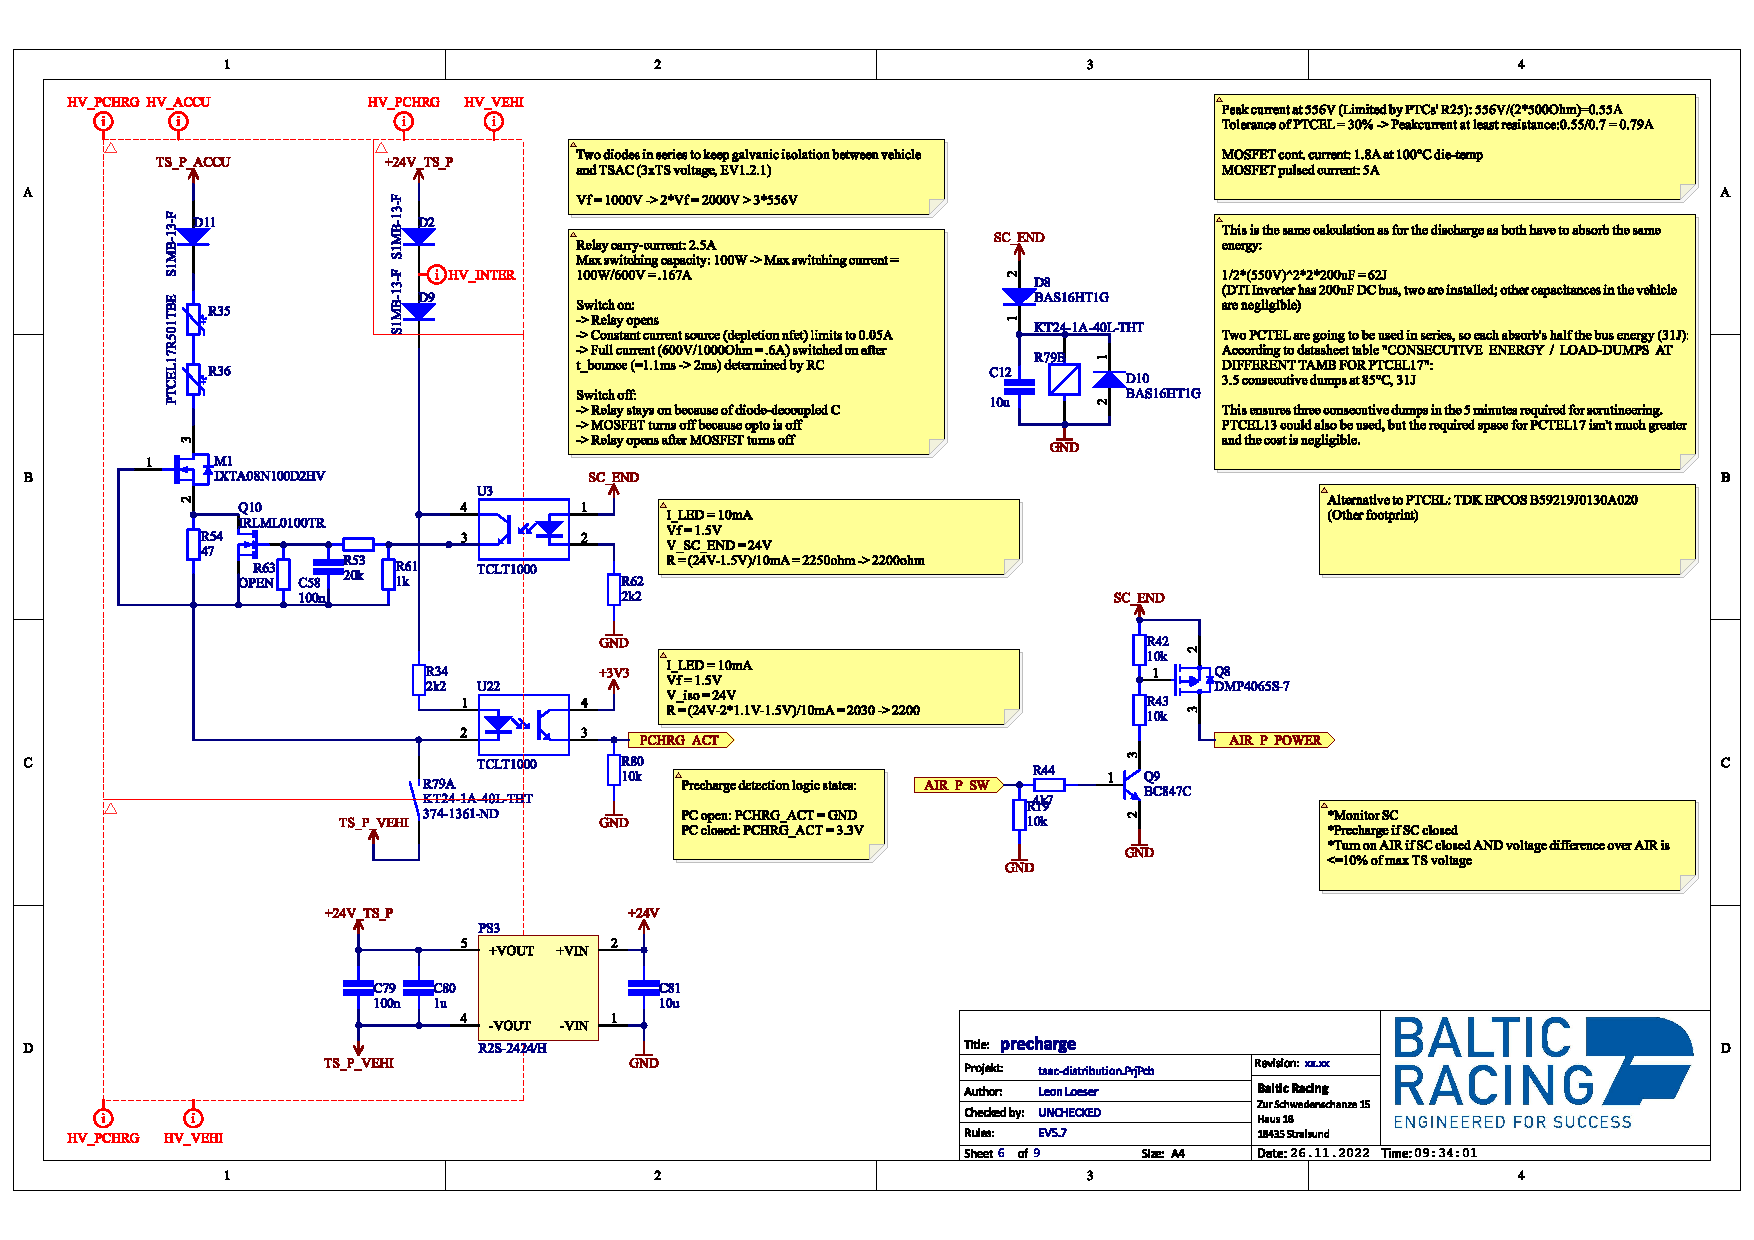
\includegraphics[width=0.7\linewidth]{bilder/Precharge_Complete}
	\caption{}
	\label{fig:prechargecomplete}
\end{figure}
\FloatBarrier

\subsubsection{AIR Detection}

\begin{figure}
	\centering
	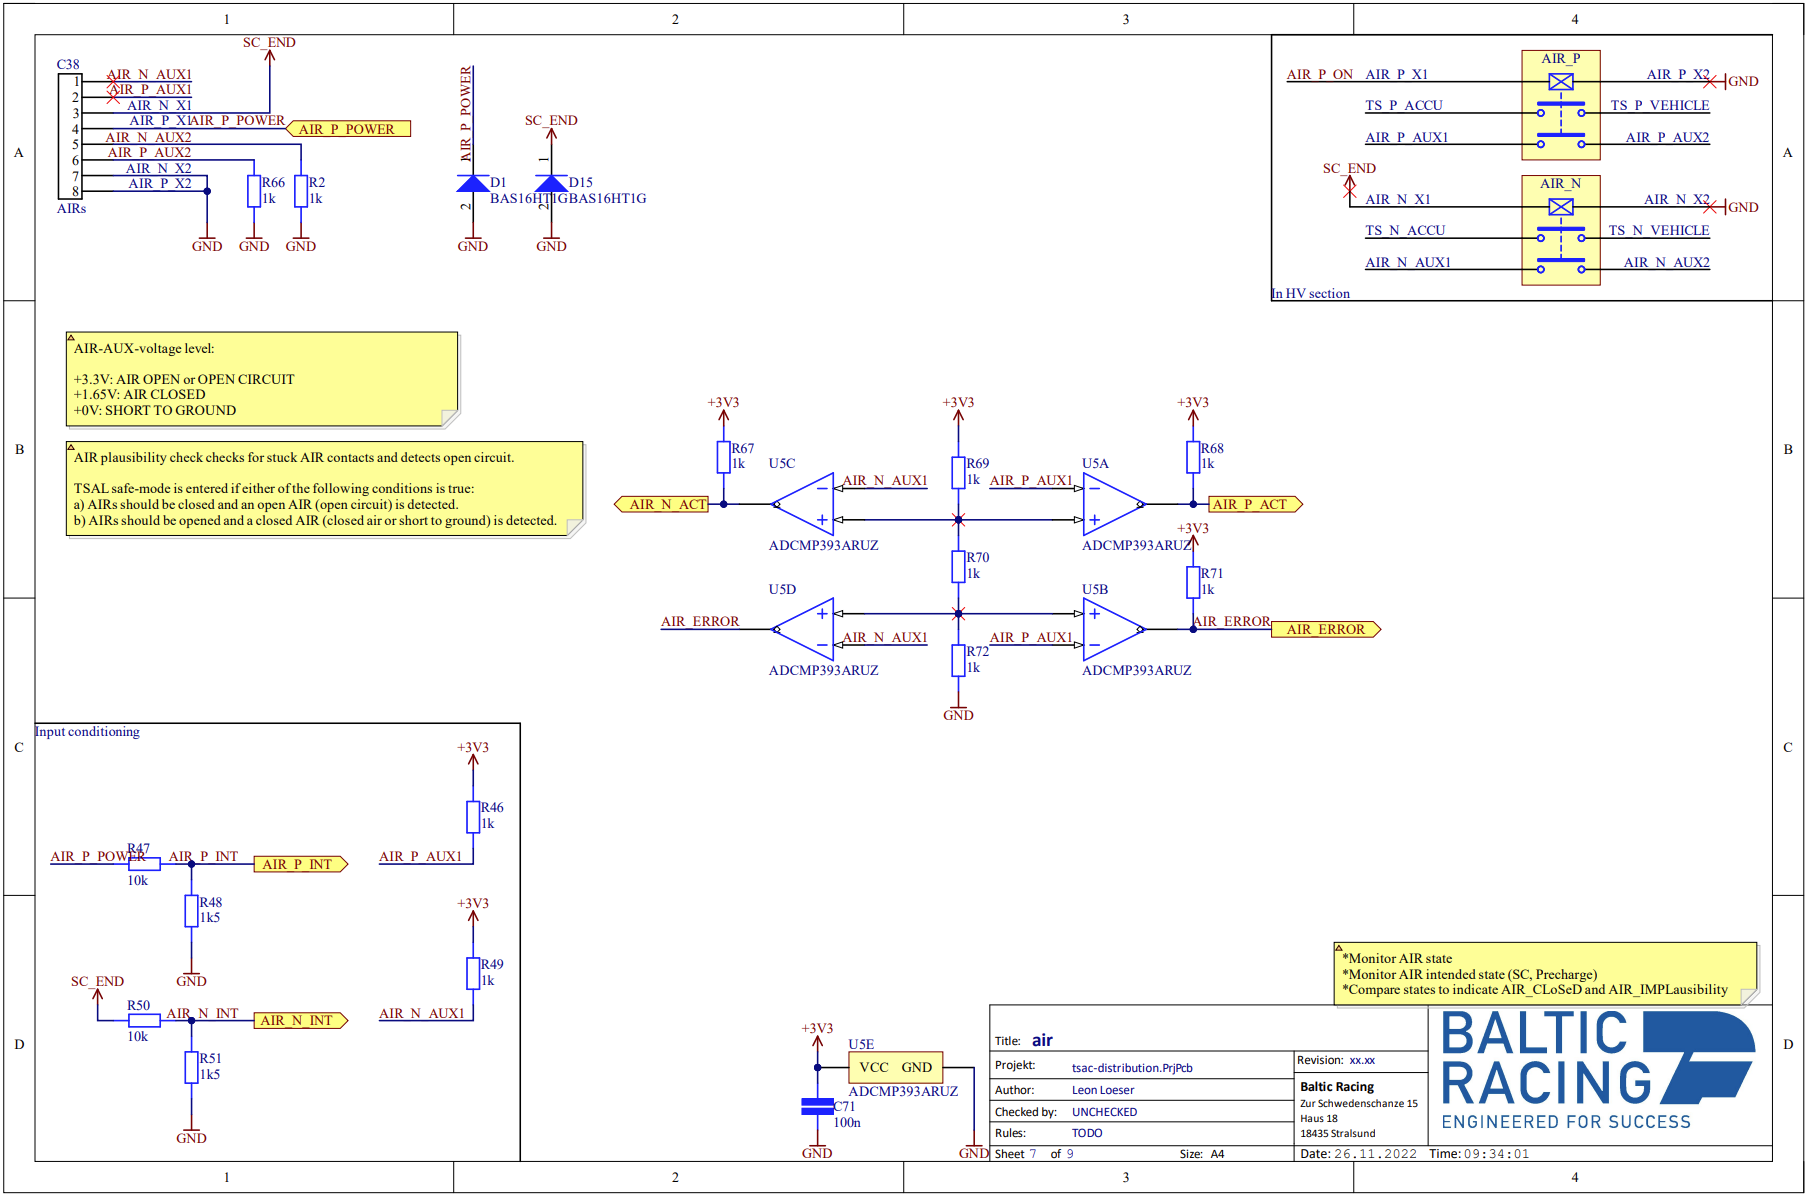
\includegraphics[width=0.7\linewidth]{bilder/AIR_conditioning}
	\caption{}
	\label{fig:airconditioning}
\end{figure}

Sinn der AIR detection ist es die Signale vom AIR in Sinnvolle Logikpegel umzusetzen welche im späteren verlauf weiter verwendet werden können. Oben rechts auf der Schematik sind die AIRs dargestellt. Relevant sind dabei die X Signale welche den Schaltzustand des Relais kontrollieren und die AUX Signale welche den Schaltzustand überwachen. Die AUX Signale werden mit 3,3V über einen Gleichwertigen 1 kOhm Spannungsteiler versorgt, so das bei geöffnetem Relais die 3,3V an AUX 1 anliegen, bei geschlossenem Relais durch den Spannungsteiler 1,65V und bei einem Kurzschluss in der Signalleitung zu Masse 0V anliegen. Diese Spannungspegel werden jetzt in einer komparatorschaltung verglichen. Die oben beiden Komparatoren geben ein High Signal aus wenn die Spannung an den AUX Kontakten kleiner ist als die Referenzspannung und damit die Relais geschlossen oder auf Masse kurzgeschlossen sind. Die beiden unteren Komparatoren geben ein Low Signal aus wenn die Spannung größer ist als die Referenzspannung und damit das Relais geschlossen oder geöffnet ist. Sofern also der tatsächliche zustand des Relais High ist un der Fehler Low kann zum Beispiel geschlussfolgert werden das jenes Relais geschlossen ist.
\FloatBarrier
\subsubsection{AMS}
Das eigentliche Batteriemanagement wird von vom LTC 6804 übernommen. hierbei handelt es sich um eine integrierte Schaltung welche speziell für die Aufgabe des batteriemanagment von Linear Technology entwickelt wurde. Relevante aufgaben dieses Chips ist die differentielle Messung der Zellspannungen im Stack. Weiter übernimmt der IC die Temperatur Messung über 5 frei nutzbare GPIO`s welche auch ADC Funktionalität unterstützen. Zu guter Letzt wird der Chip als Treiber für Mosfets benutzt welche die Zelle auf den balancing widerstand schalten. Die notwendige Kommunikation erfolgt über einen proprietären 2 drahtigen linearen isolierten SPI Bus. Jeder Chip hat dabei 4 Adressbits zur Konfigurierung. Das Kommunikationsinterface zischen dem Iso SPI und dem SPI bus des Mikrocontroller erfolgt über den LTC6820 welcher für exakt diese Aufgabe entwickelt wurde. Mit den 5 Eingängen am Chip sind nun 11 verschiedene NTC`s auszuwerten, dies geschieht mit Hilfe eines Demuxers und eines Invertierers.

Zum Verständnis der Logik ist im folgenden einmal beispielhaft der Signalablauf dargestellt.
Die Bits SEL0 und SEL1, in diesem Beispiel Low und High, vom LTC 6804 (U1) gehen auf die Eingänge A und B am Demuxer (U6). G2A und G2B sind immer auf Low gesetzt und G1 immer auf High. Mit der Tabelle \ref{Demuxer_Logiktabelle} aus dem Datenblatt wird nun der Ausgang von Y0 bis Y3 bestimmt.

\begin{figure}
	
	\centering
	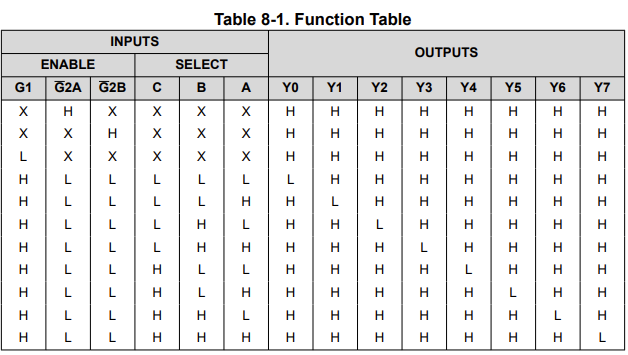
\includegraphics[width=0.3\linewidth]{bilder/AMS_demuxer_logiktabelle}
	\caption{}
	\label{Demuxer_Logiktabelle}
	\label{fig:amsdemuxerlogiktabelle}
\end{figure}

\FloatBarrier
\begin{table}
	\centering
	\begin{tabular}{|c|c|}
		\hline
		Y0 & 1 \\
		\hline
		Y1 & 1 \\
		\hline
		Y2 & 0 \\
		\hline
		Y3 & 1 \\
		\hline
	\end{tabular}
\end{table}

Diese Signale gehen nun in die beiden Invertierer U2 \& U5. Der Ausgang des Invertierers stellt die Versorgung des NTC dar.
\begin{table}
	\centering
	\begin{tabular}{|c|c|}
		\hline
		NTC-sig0 & 0 \\
		\hline
		NTC-sig0 & 0 \\
		\hline
		NTC-sig1 & 1 \\
		\hline
		NTC-sig2 & 0 \\
		\hline
		NTC-sig3 & 0 \\
		\hline
		NTC-sig4 & 0 \\
		\hline
		NTC-sig5 & 0 \\
		\hline
		NTC-sig6 & 1 \\
		\hline
		NTC-sig7 & 0 \\
		\hline
		NTC-sig8 & 0 \\
		\hline
		NTC-sig9 & 0 \\
		\hline
		NTC-sig10 & 0 \\
		\hline
		NTC-sig11 & 1 \\
		\hline
	\end{tabular}
\end{table}

\begin{figure}
	\centering
	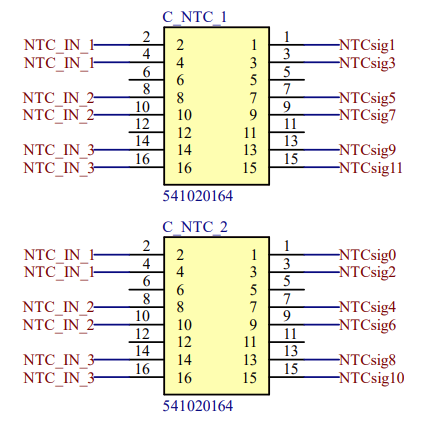
\includegraphics[width=0.3\linewidth]{bilder/AMS_NTC_steckerlayout}
	\caption{}
	\label{fig:amsntcsteckerlayout}
\end{figure}

zusammen mit dem NTC Steckerlayout ergibt dies also das an NTCin1 bis NTCin3 jeweils ein Signal von einem NTC anliegt.

In der Abbildung \ref{fig:amsbalancingschematic} ist der Balancing Aufbau der einzelnen Zellen zu sehen. Dabei werden pro Zelle immer zwei Pins der LTC6804 gebraucht, einer zum steuern des Fet`s und einer zum messen der Zellspannung. das sind respektive die S und C Pins. Die Balancing Leistung wurde auf 2 Watt festgelegt. Damit kommen wir bei einer Zellspannung von 4,2V auf einen Widerstand von ca. 10 Ohm. Zusätzlich ist parallel zu jedem Wiederstand eine LED verschaltet mit der die Aktivität des BMS im betrieb sichtbar wird.

\begin{figure}
	\centering
	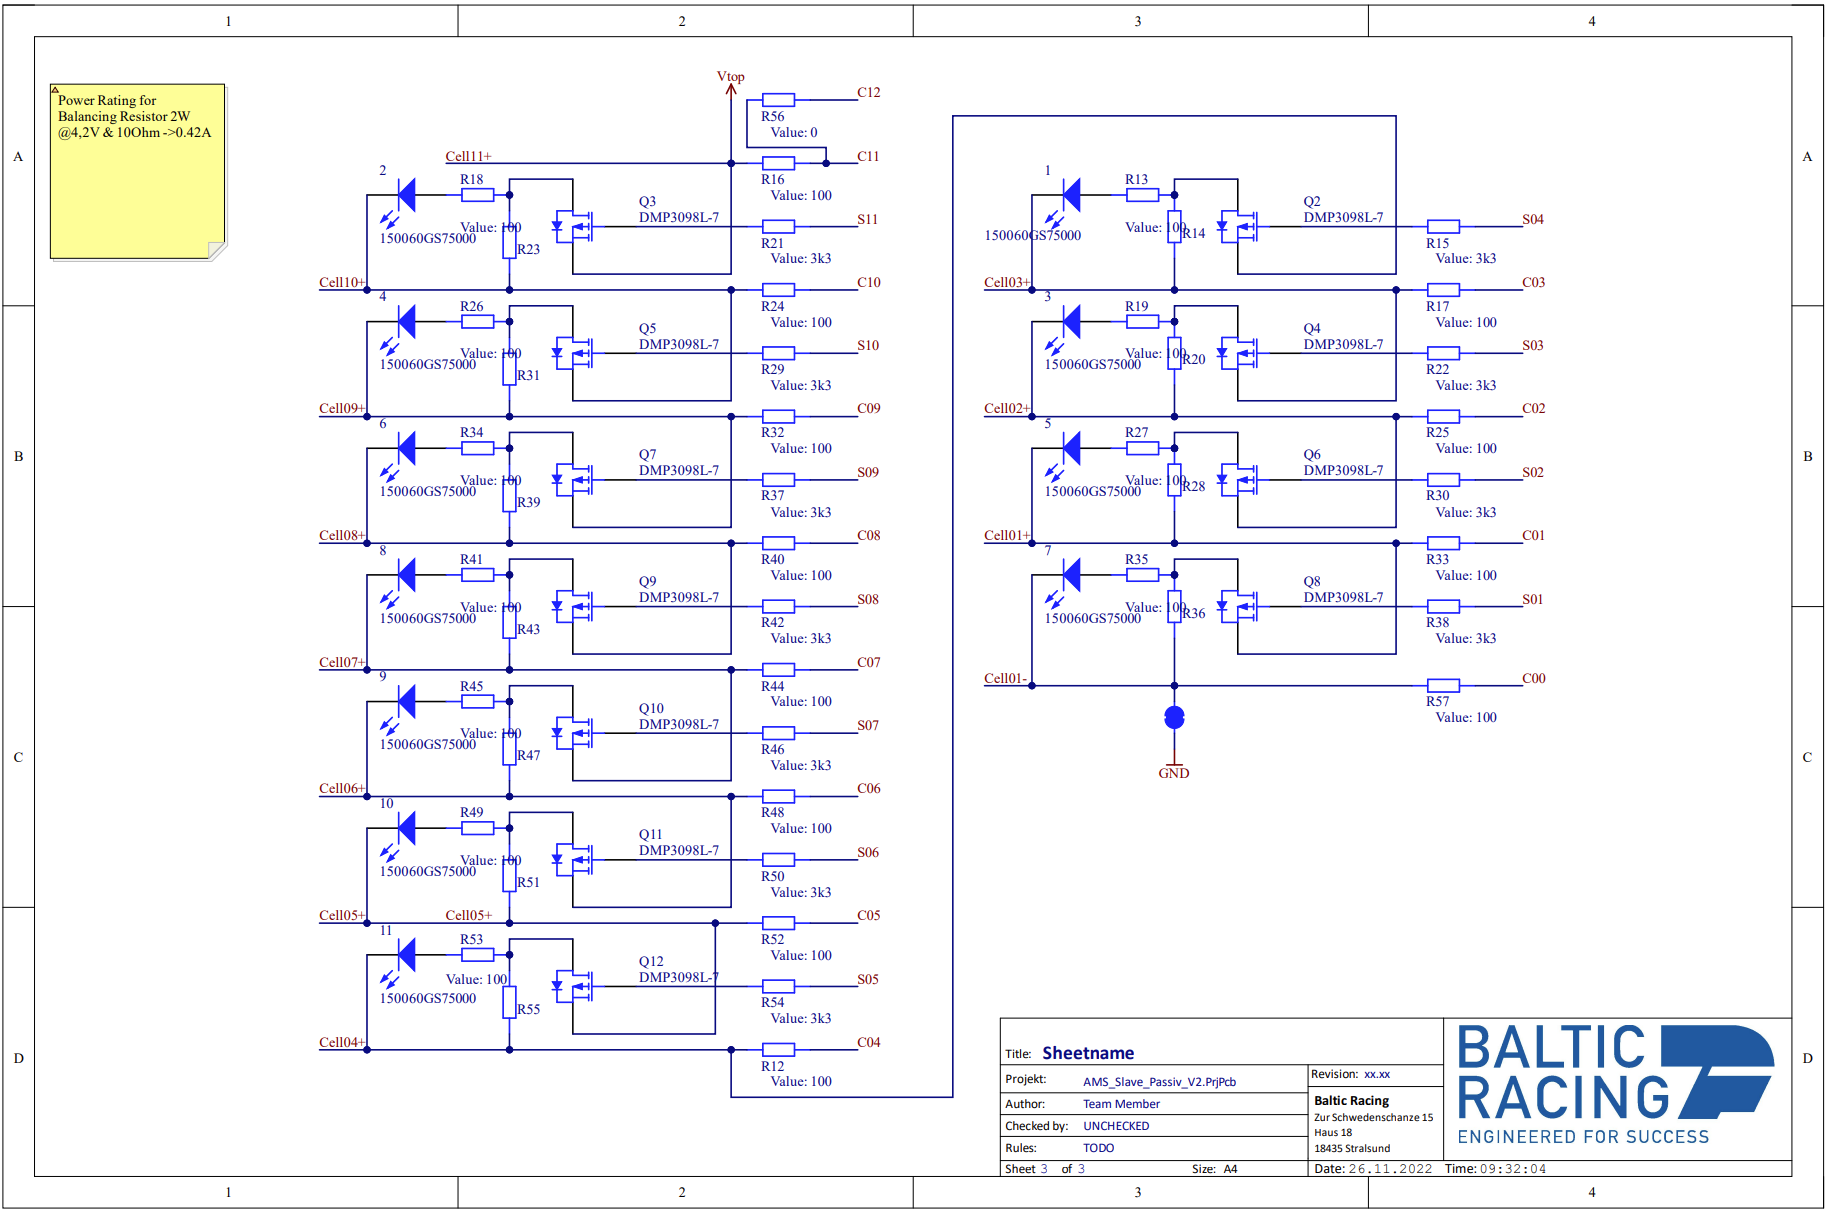
\includegraphics[width=0.7\linewidth]{bilder/AMS_Balancing_Schematic}
	\caption{}
	\label{fig:amsbalancingschematic}
\end{figure}


\begin{figure}
	\centering
	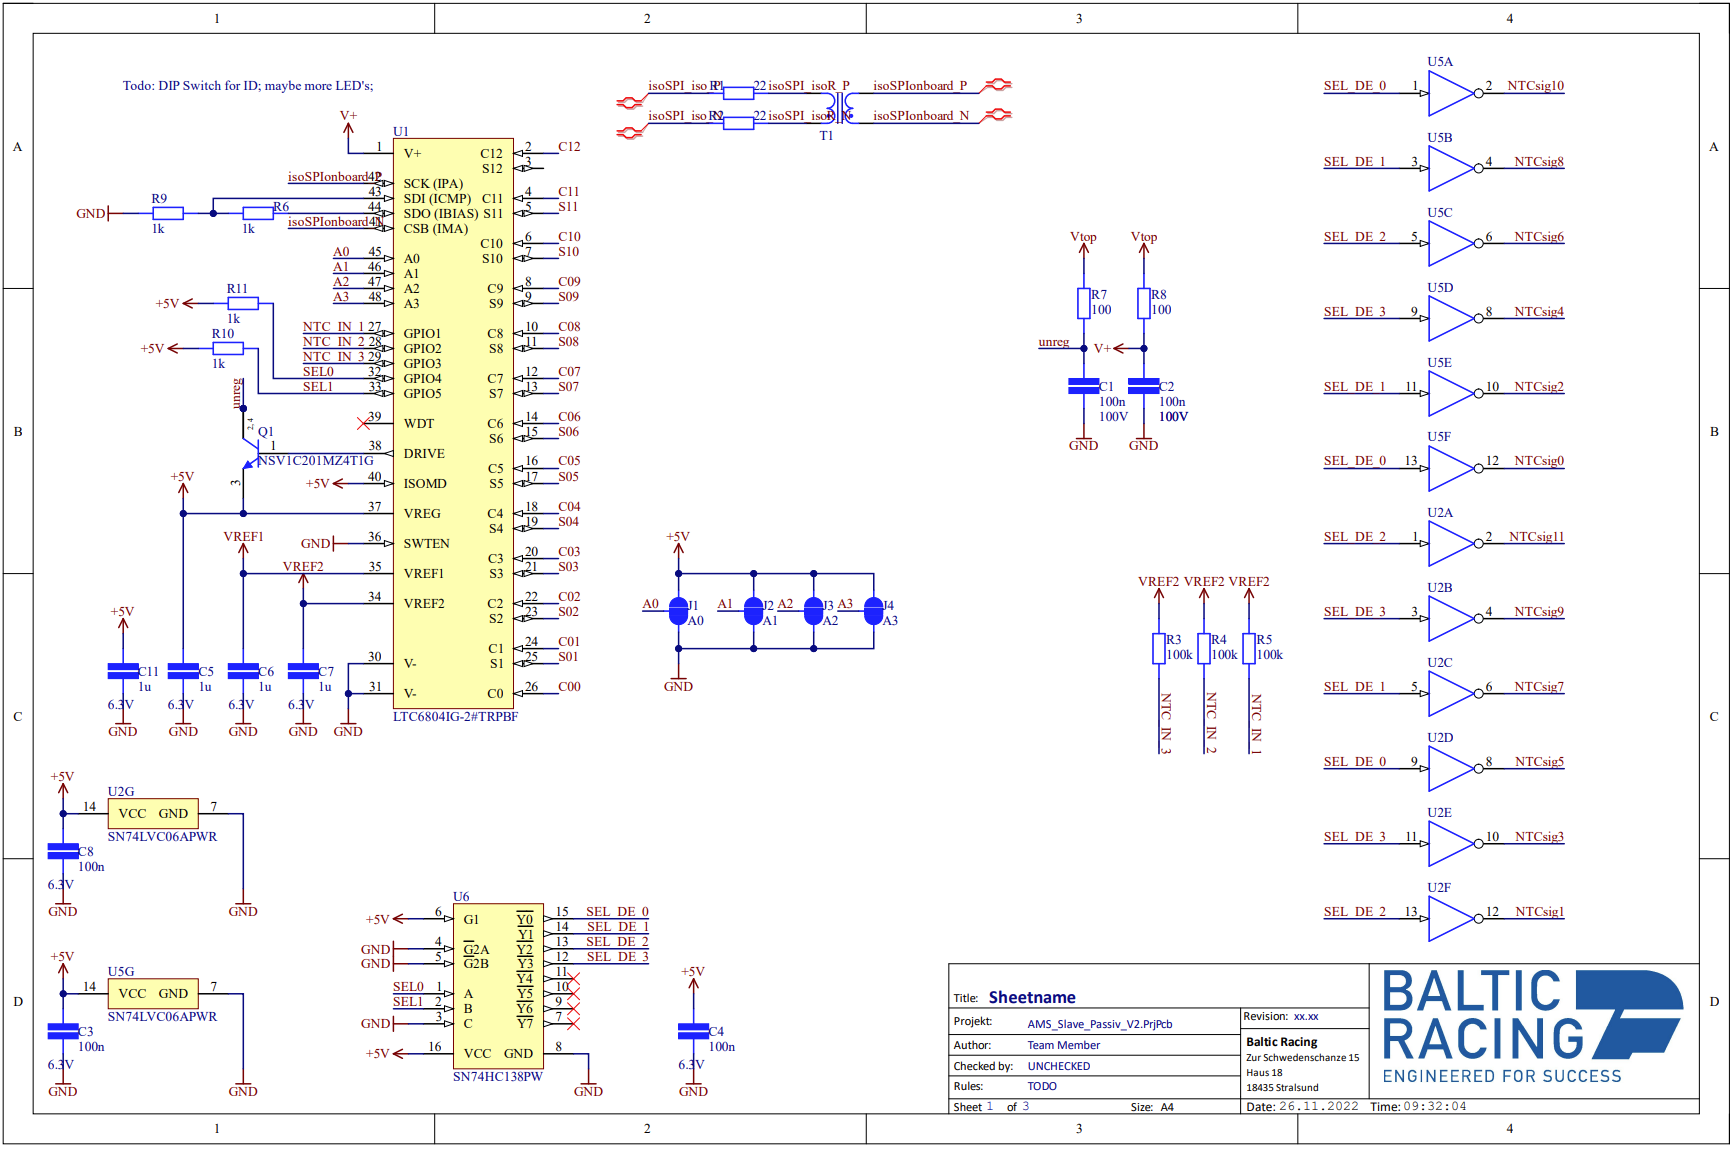
\includegraphics[width=0.7\linewidth]{bilder/AMS_slave_controller_schematic}
	\caption{}
	\label{fig:amsslavecontrollerschematic}
\end{figure}

\FloatBarrier
\subsubsection{HV Indicator}

\begin{figure}
	\centering
	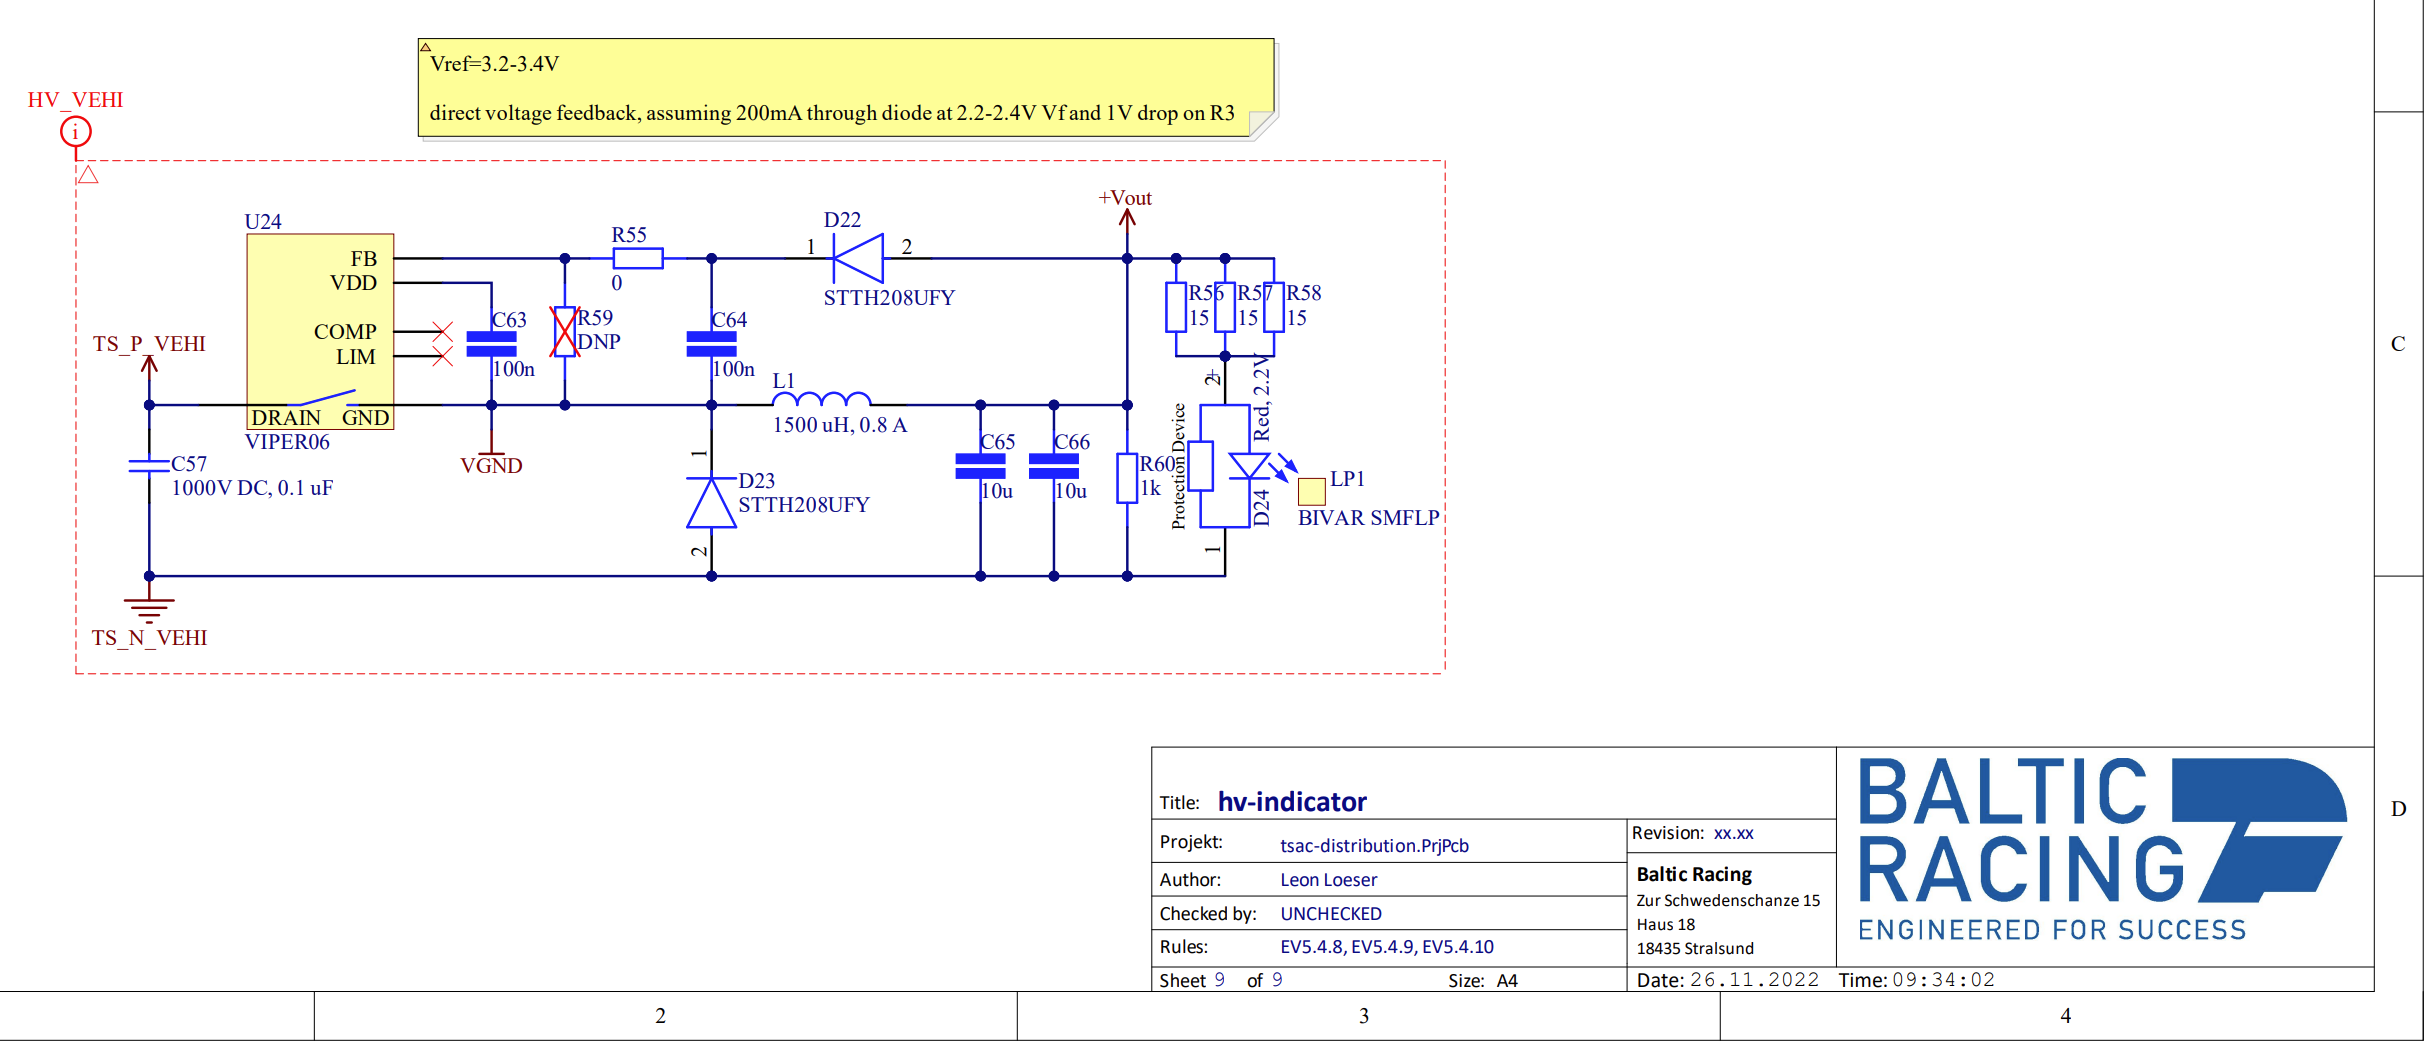
\includegraphics[width=0.7\linewidth]{bilder/HV_indicator_schematic}
	\caption{}
	\label{fig:hvindicatorschematic}
\end{figure}

Der HV Indikator ist ein rotes Licht auf dem Akkumulator, sofern an HV Terminals des Akkus eine gefährliche Spannung liegt muss dieses Licht erleuchten und dem Bediener somit anzeigen das es z.b. nicht sicher ist den Akku vom Zwischenkreis zu trennen da dieser noch unter Spannung steht. Die Anzeige erfolgt über eine Rote LED wessen licht mit einer Glasfaser von der Platine zum Deckel geleitet wird. Die Ansteuerung der LED erfolgt über einen kleinen DC Wandler, den Viper06. Dieser Wandler verfügt über einen Drain Source startup Voltage von 25-40V. Das bedeutet, bei einer Spannung in diesem Bereich beginnt der Chip zu arbeiten. Dieser Strom fließt dann zur LED so das diese zu leuchten beginnt. Die Feedback Schaltung ist direkt an den Spannungsausgang gekoppelt so das wir die interne Spannungsreferenz von 3,2 V - 3,4 V nutzen. Die Vorwiederstände vor der LED sind dementsprechend ausgelegt.

\FloatBarrier
\subsubsection{HV Messung}
Sinn der HV Messung ist es die Spannung welche am Akku als auch am Zwischenkreis anliegt erfassen und digitalisieren zu können. Dadurch kann zusammen mit dem Signal vom Stromsensor z.b. die DC Leistung bestimmt und geloggt werden. 

\begin{figure}
	\centering
	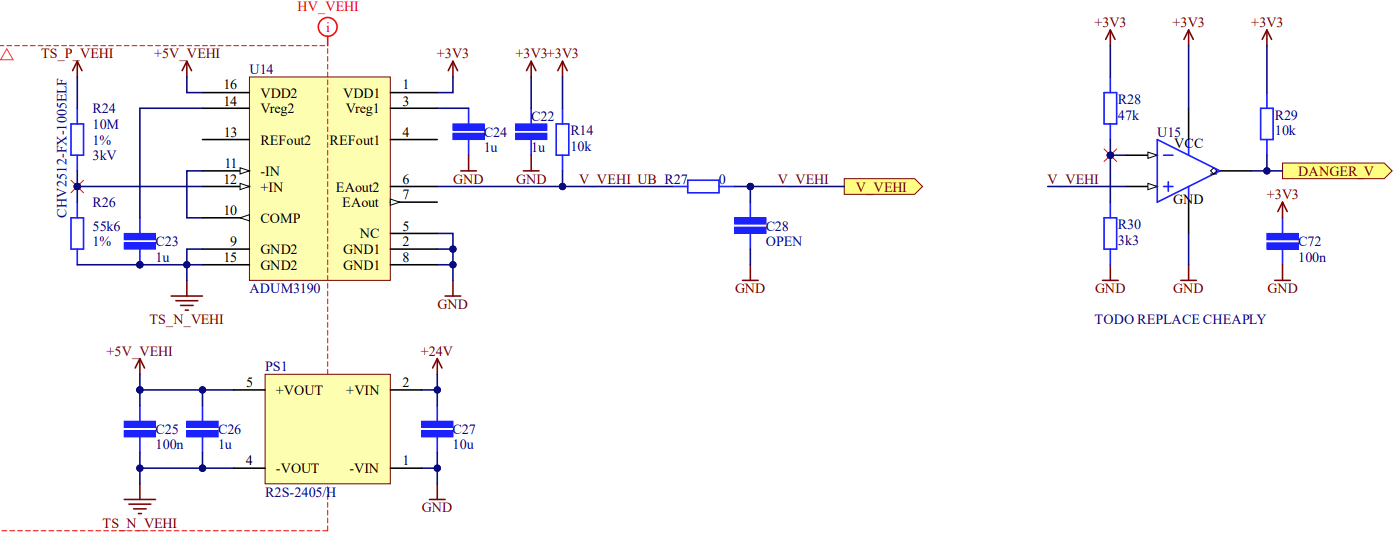
\includegraphics[width=0.7\linewidth]{bilder/HV_Measurement_PNG}
	\caption{}
	\label{fig:hvmeasurementpng}
\end{figure}

\begin{figure}
	\centering
	\includegraphics[width=0.4\linewidth]{"bilder/Blockdiagramm ADUM3190"}
	\caption{}
	\label{fig:blockdiagramm-adum3190}
\end{figure}

Kern dieser Schaltung ist der ADUM 3190. dabei handelt es sich um einen Isolierten Operationsverstärker. Der positive Eingang ist über einen Spannungsteiler mit dem HV-Kreis verbunden. Der negative Eingang ist mit dem Ausgang des OPV rückgekoppelt so das ein Spannungsfolger mit einer Verstärkung von 1 entsteht. Aus dem 10Mohm und dem 55,6kOhm widerstand ergibt sich eine Verhältnis von 179,86V im HV Kreis zu einem Volt am Eingang des OPV. Das ergibt eine maximale Eingangsspannung für die Schaltung von 593,54V da hierbei eine Ausgangsspannung von 3,3V erreicht wird. Bei dem R2S-2405/H handelt es sich um einen isolierten DC Wandler um den Chip HV seitig mit Strom zu versorgen. Die Komparatorschaltung um U15 gibt bei überschreiten der gefährlichen Spannung einen High Pegel aus. Die Spannung über den positiven Eingang der komparatorschaltung liegt bei 0,232V so das bei einer TS Spannung von größer 41,73V der High Pegel anliegen sollte. Laut Regelwerk sollte dieser Pegel spätestens bei 60V anliegen.

\FloatBarrier
\subsubsection{IMD Monitoring}

Bei dem IMD handelt es sich um ein Bender Isometer IR155-320x. Dieses Isolationsmessgerät wird von der Formula Student empfohlen und wird den Teams in der regel von dem unternehmen kostenlos zur Verfügung gestellt.
Das IMD hat zwei Ausgänge die für die Auswertung des Messergebnis relevant sind. Einmal ein digitales OK HS Signal und ein PWM Signal Mhs oder Mls je nach Variante. Das OK Signal gibt alle relevanten Informationen aus in der Form das low geht wenn z.b ein Isolationsfehler oder ein Gerätefehler erkannt wurde. Das PWM Signal ermöglicht es z.b den Fehler weiter einzugrenzen oder den aktuellen Messwert auszugeben. Dementsprechend muss das OK Signal rein analog den shutdwon circuit betätigen können während der PWM Ausgang nur Information ist und an einen Mikrocontroller angeschlossen wird. Beim startup ist das PRE als auch das CLR signal am D FlipFlop U7A Low. dadurch ist der Ausgang Q High was aufgrund der Diode D14 aber keinen Einfluss auf die restliche Schaltung hat. Die Spannung am gate des P-Channel Fet Q3 ist Low und die Spannung an der Source ist High, dadurch liegt eine negative Gate Source Spannung an so das der Fet geschlossen ist. Dementsprechend ist die Spannung an der source annähernd low. Nun sollte sofern kein Fehler seitens des IMD vorliegt das OK Signal High gehen. Dadurch öffnet der Fet Q3, gleichzeitig bleibt Q vom FlipFlop high. Nun liegt Spannung an der Basis von Q5 und es fließt ein Basis Emitter Strom so das auch ein Collector Emittor Strom fließen kann. Dadurch liegt zusammen mit den Widerständen R37 und R38 eine negative Gate Source Spannung an Q4 an so das der P Channel Fet durchschaltet und der Shutdown Circuit geschlossen wird. Daraufhin schaltet der POR high so das der zustand vom Flip Flop gespeichert wird und somit High bleibt. Wenn das Ok Signal nun Low geht weil ein Fehler auftritt, wird Q auf Low gesetzt. Wenn Ok nun wieder High geht weil z.b. der Fehler wieder aufgehoben ist, beispielsweise durch einen Wackelkontakt an einem der Messeingänge wird der aktuelle zustand gespeichert welcher Low ist, so das die Schaltung sich nicht mehr selbst zurücksetzen kann. Ein Wiedereinschalten ist nur durch den POR möglich.


\begin{figure}
	\centering
	\includegraphics[width=0.7\linewidth]{"bilder/IMD Monitoring schematic"}
	\caption{}
	\label{fig:imd-monitoring-schematic}
\end{figure}


\FloatBarrier
\subsection{HV DCDC}
Visio blockmodell
Erklärung ACFC
Berechnung excel etwas aufhübschen und anhängen
Teilberechnungen erklären

\FloatBarrier
\section{HV Distribution}
Bei der HV Distribution handelt es sich um eine Box welche mittig hinter dem Fahrer angeordnet ist. Diese Box beinhaltet alles an HV Elektrik was nicht im Akkumulator oder in den Umrichtern zu finden ist. Hier ist auch der Service Disconnect untergebracht.

\FloatBarrier
\subsection{TSMP}
Die Tractive System Measuring Points befinden sich seitlich am Fahrzeug wo auch der Hauptschalter zu finden ist. Sie stellen eine genormte Schnittstelle dar um mit einem Duspol, oder Multimeter an die Spannung des Tractive Systems gelangen zu können. Hierbei müssen laut Regelwerk geschirmte Bananenstecker eingesetzt werden. Weiter muss für die Buchsen am Fahrzeug eine Abdeckkappe oder Blindstecker vorgesehen werden. Zur Absicherung der TSMP müssen diese mit Widerständen in reihe an den HV Kreis angebunden werden. Das Regelwerk sieht hierbei in unserem Spannungsbereich 15k$\Omega$ vor. Der Kritische wert wonach die TSMP ausgelegt werden müssen ist das Leistungsrating, da diese auf kontinuierlichen Kurzschluss ausgelegt sein müssen.

Eine Formel zu Berechnung der Leistung am Widerstand ist folgende

\begin{equation}
	\label{eqn:Leistung am Wiederstand}
	\glsc{symb:P_elektrisch} = \glsc{symb:I}^{2} * \glsc{symb:R}
\end{equation}

Der Strom errechnet sich aus.

\begin{equation}
	\label{eqn:URI}
	\glsc{symb:U} = \glsc{symb:R}^{2} * \glsc{symb:I}
\end{equation}

Umgestellt nach I.

\begin{equation}
	\label{eqn:IUR}
	\glsc{symb:I} = \dfrac{\glsc{symb:U}} {\glsc{symb:R}}
\end{equation}

Da im Kurzschlussfall die Spannung über beide Widerstände anliegt, verdoppelt sich der Widerstand.

\begin{table}[h]
	\centering
	\begin{tabular}{|c|c|c|}
		\hline
		\multicolumn{3}{|c|}{Eingangsparameter} \\
		\hline
		\glsc{symb:R} & 15 & \ensuremath{k\Omega} \\
		\hline
		\glsc{symb:U} & 600 & \ensuremath{V} \\
		\hline
		\multicolumn{3}{|c|}{Ergebnisse} \\
		\hline
		\glsc{symb:I} & 20 & \ensuremath{mA} \\
		\hline
		\glsc{symb:P_elektrisch} & 12 & \ensuremath{W} \\
		\hline
	\end{tabular}
\end{table}

Daraus schlussfolgert sich das die 15k$\Omega$ Widerstände mit einem Leistungsrating von mindestens 12 W benötigt werden.

\FloatBarrier
\subsection{BSPD}

\begin{figure}
	\centering
	\includegraphics[width=0.7\linewidth]{"bilder/BSPD Blockdiagramm"}
	\caption{}
	\label{fig:bspd-blockdiagramm}
\end{figure}

Die Aufgabe des BSPD ist es das Fahrzeug in dem Fall einer Störung des Gaspedales in einen Sicheren zustand zu überführen. Hierfür wird der Strom zu den Umrichtern als auch der Bremsdruck gemessen und beim eintreten eines im Regelwerk definierten schwellwertes für das gleichzeitige auftreten beider Signale muss das abschalten des Antriebes erfolgen. Das Folgende Blockdiagramm soll einen Überblick über den signalfluss ermöglichen.

Bei den Eingangsignalen handelt es sich um analoge spannungen. Für Sigfnalaufbereitung oder auch Digitalisierung der Signale werden Schitds Trigger einbgesetzt, Die Logik besteht aus diversen Logikgattern und die Set/reset Schaltung besteht aus RC Gliedern mit nachgeschaltetetn schmidt triggern. Beim Shutdowncircuit handelt es sich um ein Solid State Relay welches von der BSPD Logik schlussendlich angestuert werden soll, ein öffnen des Shutdwon circuit führt damnit zu einem Herunterfahren des Antriebes.

Zur Auslegung von Schmidt Triggern
\begin{figure}
	\centering
	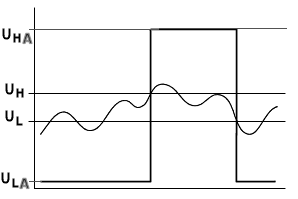
\includegraphics[width=0.5\linewidth]{bilder/Schmitt-trigger-diagramm.png}
	\caption{}
	\label{fig:schmitt-trigger-diagramm}
\end{figure}

Die Funktionsweise eines Schmitt Trigger kann anhand des Bildes erkannt werden. Er ermöglicht es ein analoges Signal in ein Digitales umzuwandeln, dabei ist es möglich festzulegen welche Spannungspegel am Ausgang des Schmitt Trigger anliegen (\glsc{symb:U_HA} und \glsc{symb:U_LA}) und bei welchen Spannungspegeln der Trigger High respektive Low schalten soll (\glsc{symb:U_H}und \glsc{symb:U_L}). Das vorliegen unterschiedilcher Pegel zum Schalten wird Hysterese genannt. Grund für das vorliegen ist das verhindern des rapiden Umschaltens zwischen High und Low direkt an dem Schwellwert aufgrund von Signalrauschen.

\begin{figure}
	\centering
	\includegraphics[width=0.7\linewidth]{"bilder/TPS Failure detection"}
	\caption{}
	\label{fig:tps-failure-detection}
\end{figure}

\begin{figure}
	\centering
	\includegraphics[width=0.5\linewidth]{"bilder/nichtinvertierender Trigger"}
	\caption{}
	\label{fig:nichtinvertierender-trigger}
\end{figure}

Folgend Beispielhaft die Auslegung eines Nicht Invertierenden Schmitt Triggers wie er im Bild unten zu sehen ist. Die andere Ausführung ist die eines Invertierenden.

Zur Berechnung sollten sich \glsc{symb:U_HA} und \glsc{symb:U_LA} sowie \glsc{symb:U_H} und \glsc{symb:U_L} aus dem Betriebsfall ergeben. R\textsubscript{1} sowie R\textsubscript{3} können frei gewählt werden. R\textsubscript{1} ist hierbei der Verbund aus R\textsubscript{3} und R\textsubscript{4}.

Die beiden folgenden Gleichung liegen zu Grunde

\begin{equation}
	\label{eqn:Obere Hysteresespannung Schmitt Trigger}
	\glsc{symb:U_H} = \glsc{symb:U_ref} + (\glsc{symb:U_HA} - \glsc{symb:U_ref}) * \dfrac{R\textsubscript{1}} {R\textsubscript{1}+R\textsubscript{2}}
	mit R\textsubscript{1}=\dfrac{R\textsubscript{3}*R\textsubscript{4}}{R\textsubscript{3}+R\textsubscript{4}}
\end{equation}

Und

\begin{equation}
	\label{eqn:Untere Hysteresespannung Schmitt Trigger}
	\glsc{symb:U_L}=\glsc{symb:U_ref}-(\glsc{symb:U_ref}-\glsc{symb:U_HA})*\dfrac{R\textsubscript{1}}{R\textsubscript{1}+R\textsubscript{2}}
\end{equation}

Mit den folgenden Gleichungen lassen sich R\textsubscript{2} und R\textsubscript{4} bestimmen

\begin{equation}
	\label{eqn:Berechnung R2 Schmitt Trigger}
	R\textsubscript{2} = R\textsubscript{1} * \dfrac{\glsc{symb:U_HA} - \glsc{symb:U_LA}} {\glsc{symb:U_H} - \glsc{symb:U_L}}
\end{equation}

\begin{equation}
	\label{eqn:Berechnung Uref Schmitt Trigger}
	\glsc{symb:U_ref} = (\glsc{symb:U_H} - \glsc{symb:U_LA}) * \dfrac{R\textsubscript{2}} {R\textsubscript{1} + R\textsubscript{2}} + \glsc{symb:U_LA}
\end{equation}

\begin{equation}
	\label{eqn:Berechnung R4 Schmitt Trigger}
	R\textsubscript{4} = R\textsubscript{3} * \dfrac{\glsc{symb:VCC}-\glsc{symb:U_ref}} {\glsc{symb:U_ref}}
\end{equation}

\begin{figure}
	\centering
	\includegraphics[width=0.7\linewidth]{"bilder/BSPD Integrator"}
	\caption{}
	\label{fig:bspd-integrator}
\end{figure}

Zur Auslegung der Zeitsteuerung

Die Zeitsteuerung besteht aus einem Kondensator C2 welcher über den Widerstand R20 geladen wird, einer Diode D3 um Rückkopplung zu vermeiden, einem Widerstand R23 um den Kondensator langsam zu entladen, einem Spannungsfolger OP2 um die Schaltung von dem nachgeschalteten Schmitt Trigger zu entkoppeln und einem Transistor T3 der den Kondensator in kurzer Zeit bei Bedarf entladen kann.

Für die Berechnung ist die Ladezeit des Kondensators über den Widerstand R20 bis zur Schaltspannung des Schmitt Triggers zu ermitteln. Dies lässt sich mit folgender Gleichung Lösen. 

\begin{equation}
	\label{eqn:Ladezeit Kondensator}
	\glsc{symb:U_a}=\glsc{symb:U_e}*(1-\glsc{symb:e}^{\dfrac{1}{\glsc{symb:R}*\glsc{symb:C}}*\glsc{symb:t}})
\end{equation}

Alternativ kann der Schmitt Trigger aber auch auf 0,63 fache der Eingangsspannung gesetzt werden was der einfachen Zeitkonstante des RC Gliedes entspricht. Damit bestimmt sich C wie folgt.

\begin{equation}
	\label{eqn:Zeitkonstante Kondensator}
	\glsc{symb:C}=\dfrac{\glsc{symb:tau}}{\glsc{symb:R}}
\end{equation}

Mit Beispielhaften Auslegeparametern ergeben sich folgende Werte.

\begin{table}[h]
	\centering
	\begin{tabular}{|c|c|c|}
		\hline
		\multicolumn{3}{|c|}{Eingangsparameter} \\
		\hline
		\glsc{symb:tau} & 0,5 & \ensuremath{s} \\
		\hline
		\glsc{symb:R} & 100 & \ensuremath{k\Omega} \\
		\hline
		\multicolumn{3}{|c|}{Ergebnisse} \\
		\hline
		\glsc{symb:C} & 5 & \ensuremath{uF} \\
		\hline
	\end{tabular}
\end{table}

Das BSPD-Sensorboard hat zum Zweck einen Stromsensor zu kreieren der ein Stromsignal von 0-100A in ein Spannungssignal von 0.5-4.5V über den Bereich von 0-10A zu erzeugen. Die 0.5V Offset haben zum ziel eine Kurzschlusserkennung auf Masse als auch auf Versorgung zu ermöglichen. Der relevante Messbereich von 0-10A entsteht aus den Regelwerksanforderungen die vorgeben das der Fehlerzustand bei einer abgerufenen Leistung größer 5kW eingestellt werden muss was bei 600V in einem Strom von 8,3A resultiert. Dieser Bereich muss möglichst robust ausgewertet werden können.

Zur genauen Funktion, U1 ist ein Hall Effekt Stromsensor mit einem Übersetzungsfaktor von 1000. Heißt 10A ergeben 10mA Stromfluss am Ausgang. Der Widerstand R2 ist so gewählt das bei einem Strom von 10mA, 5V über den Widerstand abfallen und wir so in den Messbereich kommen. Der Widerstand R1 ermöglicht nun das konstante einspeisen von ca. 0,5V und die Diode das Begrenzen der max. Spannung auf 4,5V.

\begin{figure}
	\centering
	\includegraphics[width=0.7\linewidth]{"bilder/Sensorboard Schaltung"}
	\caption{}
	\label{fig:sensorboard-schaltung}
\end{figure}

\FloatBarrier
\subsection{Discharge}
Die Discharge Schaltung soll bei Abschalten des Fahrzeug die Zwischenkreiskondensatoren entladen. Ziel ist es das System möglichst schnell in einen Spannungsfreien und damit sicheren Zustand zu überführen.
\begin{figure}
	\centering
	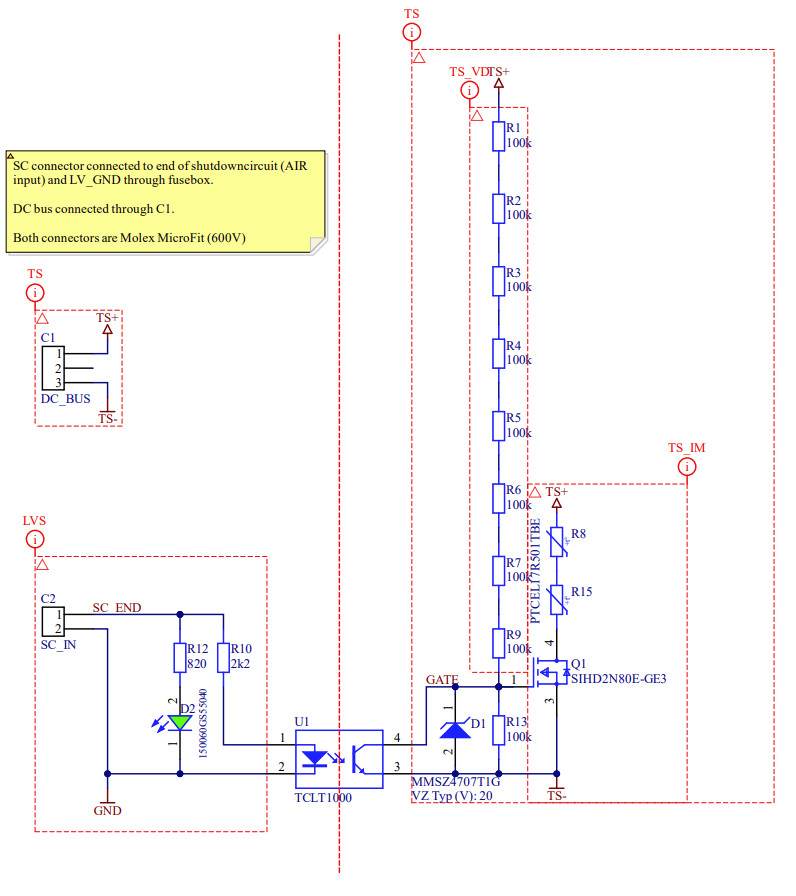
\includegraphics[width=0.7\linewidth]{bilder/Discharge}
	\caption{}
	\label{fig:discharge}
\end{figure}

Dies kann mit Hilfe von PTC Widerständen geschehen. Das Regelwerk sieht vor das der Zwischenkreis in maximal 5s auf 60VDC oder weniger zu bringen ist. Dies muss für 3 aufeinanderfolgende Entladevorgänge möglich sein. 

Die Ansteuerung erfolgt über den SDC welcher über den Steckverbinder C2 eingebunden ist. Von dort wird der Optokoppler U1 bestromt. Dieser Steuert Strom vom Gate des Mosfets Q1 weg Richtung TS- so das der Mosfet öffnet. Wenn der SDC geöffnet wird, steigt die Spannung am Gate auf 20V und der Mosfet steuert TS+ auf TS- über die PTC Wiederstände durch. Dadurch wird die Spannung im zwischenkreis in den PTC elementen abgebaut.

Die Formel für die Berechnung der PTC Elemenete ist dem Datenblatt für die PTCEL Serie der Firma Vishay zu entnehmen.

\begin{equation}
	\label{eqn:PTC Berechnung}
	\glsc{symb:N_PTC}=\dfrac{\glsc{symb:N_dump} * \glsc{symb:K} * \glsc{symb:C} * \glsc{symb:U}^{2}} {2 * \glsc{symb:R} * \glsc{symb:C_th} * (\glsc{symb:T_SW} - \glsc{symb:T_u})}
\end{equation}

\begin{table}[h]
	\centering
	\begin{tabular}{|c|c|c|c|}
		\hline
		\multicolumn{4}{|c|}{Eingangsparameter} \\
		\hline
		\glsc{symb:T_SW} & 130 & \ensuremath{°C} & Datenblatt Wiederstandsverlauf \\
		\hline
		\glsc{symb:K} & 1 & \ensuremath{-} & Datenblatt -> DC \\
		\hline
		\glsc{symb:C_th} & 2,3 & \ensuremath{J/K} & Datenblatt -> PTCEL17 \\
		\hline
		\glsc{symb:T_u} & 60 & \ensuremath{°C} & Worst Case \\
		\hline
		\glsc{symb:C} & 400 & \ensuremath{uF} & 2x DTI 500 Kapazität \\
		\hline
		\glsc{symb:U} & 600 & \ensuremath{V} & \\
		\hline
		\glsc{symb:N_dump} & 4 & \ensuremath{-} & min 3 Regelwerk\\
		\hline
		\multicolumn{4}{|c|}{Ergebnisse} \\
		\hline
		\glsc{symb:N_PTC} & 1,79 & \ensuremath{-} &  \\
		\hline
	\end{tabular}
\end{table}

Damit ergibt sich das 2 PTC`s des Typ 17R251 oder 17R501 verwendet werden müssen. 

Die Entladezeit kann wie beim BSPD über die bestimmt werden, in diesem Fall näherungsweise über die 3 fache Zeitkonstante. Damit ergibt sich eine Entladezeit von max. 1,2s.

\FloatBarrier
\section{TSAL}
Das Tractive System Activation Light ist eine Lampe im Mainhoop die 360 Grad rundherum zum Fahrzeug anzeigt ob das tractive system eingeschaltet ist oder nicht und ob ein fehler vorliegt. Damit ergeben sich drei Zustände, Tsal Rot blinkend heißt TS on, TSAL grün leuchtend heißt TS off und Tsal aus heißt entweder Low Volatge system ausgeschaltet oder fehler im TS. Die gesamte logik ist dabei in nicht programmierbaren bausteinen aka mikrocontrollern o.ä. umzusetzen.

\FloatBarrier
\subsection{Logik auf Discharge}
\label{sec: TSAL Logik Discharge}
\begin{figure}
	\centering
	\includegraphics[width=0.7\linewidth]{"bilder/Binäre Spannungserkennung"}
	\caption{}
	\label{fig:binare-spannungserkennung}
\end{figure}

Das Herz der Schaltung ist ein Verarmungstyp N-Fet. Wenn die Gate Source Spannung V\textsubscript{GS} = 0 V ist, dann lässt dieser Fet Strom durch. Ab einer Spannung von 47V wird die Zehner diode durchbrochen und ein Strom fließt, dieser Strom verursacht einen Spannungsabfall am Wiederstand R18 von ca. 2,2V bei einem mA so das V\textsubscript{GS} negativ wird und der Fet den Stromfluss zu begrenzen beginnt. Der Fet agiert zusammen mit dem Widerstand wie eine Konstantstromquelle. Diese Steuert den Optokoppler durch so das wir auf der LV Seite ein Signal erzeugt haben.

\FloatBarrier
\subsection{Logik auf AMS Master}

Nachdem jetzt die diversen Signale für den Zustand der AIR`s etc. vorliegen geht es darum sie logisch miteinander zu verschalten. Zuerst einmal wird dafür in U8a-c verglichen ob die vorhergesehen und tatsächlichen Zustände für die Relais übereinstimmen. Die XOR Gatter geben dabei immer einen High Pegel und damit einen Fehlerzustand aus wenn dies nicht der Fall ist. Zweitens gilt es nun zu plausibilisieren ob auch Spannung auf dem System anliegt. Sofern entweder der Precharge oder das positive AIR und das negative AIR geschlossen ist bedeutet dies das der Stromkreis geschlossen ist. Damit sollte Spannung anliegen. Da die Relais Signale bereits plausibilisiert wurden geht es bei dieser Schaltung nur darum zu prüfen ob das Spannungssignal etwas anzeigt wenn dies vom Relais Zustand her der Fall sein sollte. Der Fehlerzustand tritt in der Schaltung nur ein wenn die Ausgänge von U11A und U12A High sind was wiederum dadurch hervorgerufen wird, wenn bei U11A das Signal vom Precharge oder das vom positiven AIR High ist und bei U12A das Signal vom negativen AIR high ist und das Danger V Signal Low ist. Anschließend werden all diese Signale noch mit dem AIR error Ausgang verodert und in den Latch gegeben. Der Latch besteht hauptsächlich aus dem FlipFlop U26A. Der Sinn dieses ist, das wenn ein Fehler gesetzt wird dieser auch permanent bestehen bleibt und das System sich nicht selbst zurücksetzten kann. Um beim einschalten des Systems unplausible Zustände abzufangen befindet sich ein RC Glied am CLR Eingang des FlipFlop so das dieser solange keine Signale annimmt bis das System den stationären Zustand erreicht hat. Nun gibt es noch an U9B das TSon Signal welches eine veroderung der verschiedenen Relais- und des Spannungssignales darstellt. Heißt wenn irgendwas mit den AIR`s passiert oder Spannung auf dem System liegt ist das TSon. Der Ausgang des Error Latches und des TSon Signales wird nun in ein Nor Gatter gegeben so das der GRN on zustand der das TSal grün aufleuchteten lässt nur eintritt wenn was TS nicht on ist und kein Fehler vorliegt. Weiter ist das Signal noch mit dem POR verundet so, dass das Grün Signal erst aufleuchtet wenn das System auch tatsächlich arbeitet.

\begin{figure}
	\centering
	\includegraphics[width=0.7\linewidth]{"bilder/TSAL Logik AMS Master"}
	\caption{}
	\label{fig:tsal-logik-ams-master}
\end{figure}

\FloatBarrier
\subsection{Schaltung auf TSAL}

	% Autor: Lukas Deeken
% Letzte Bearbeitung: 01.05.2022

\chapter{Elektromechanische Systeme}

\section{Akkumulator}
An dieser Stelle geht mein Dank an Tim Schweers, der dieses Projekt besonders in der mechanischen Auslegung und der Konstruktion so tatkräftig mitgetragen hat.

\subsection{Die Akkuzelle}

Wichtig bei der Zellenauswahl ist das stets jede individuelle Zelle für sich begutachtet werden muss. Es gibt bei den diversen Bauformen und chemischen Zusammensetzungen gewissen Tendenzen welche im Folgenden erläutert werden. Jedoch ist die Überlappung dieser Eigenschaften in der Regel so groß das sich augenscheinlich vollkommen unterschiedliche Zellen für einen ähnlichen Einsatzzweck eignen.
\FloatBarrier
\subsubsection{Vergleich der Speicherarten}

Im nachfolgenden wird die zuerst die Energie berechnet die ein Formula Student Fahrzeug bei einem Bremsvorgang freisetzt und damit die Energie die man speichern können müsste um mit der Speicherform auf sinnvolle Art und Weise eine Rekuperation umzusetzen. Im Anschluss wird diese Energie in eine ungefähre Masse umgesetzt um zu zeigen inwiefern sich diese Form der Energiespeicherung für den Einsatz eignet. Im nachfolgenden wird die Masse bestimmt um \ensuremath{6 KWh} Energie zu speichern da, dies der Energieverbrauch eines Formula Student Fahrzeuges in der Disziplin des Endurance ist. Dieser Wert wurde im Rahmen eines Benchmarkings mit den Fahrzeugen anderer Teams über die letzten Jahre 2016 bis 2019, sowie einer \acfirst{LTS} errechnet. Die \ac{LTS} entstand im Rahmen einer vorherigen Projektarbeit. \cite{DeeDor2022}
\\
\\
Im folgenden errechnen wir die Energie welche bei einem durchschnittlich Bremsvorgang eines Formula Student Fahrzeug aufgenommen werden müsste. 

\begin{equation}
\glsc{symb:E_kin} = \dfrac{1}{2} * \glsc{symb:m} * \glsc{symb:v}^2
\end{equation}

\begin{table}[h]
	\centering
	\caption{Bremsvorgang Berechnung}
	\begin{tabular}{|c|c|c|}
		\hline
		\multicolumn{3}{|c|}{Eingangsparameter} \\
		\hline
		\glsc{symb:m}\textsubscript{Fahrzeug} & 300 & \ensuremath{m/s}\\
		\hline
		\glsc{symb:v}\textsubscript{Start} & 30 & \ensuremath{m/s}\\
		\hline
		\glsc{symb:v}\textsubscript{end} & 5 & \ensuremath{m/s}\\
		\hline
		\multicolumn{3}{|c|}{Ergebnisse} \\
		\hline
		\glsc{symb:E_kin} & 93,8 & \ensuremath{KJ}\\
		\hline
	\end{tabular}
\end{table}

\textbf{Physikalische Speicher (Kondensatoren)}\\
Kondensatoren erreichen ein sehr hohes Leistungsgewicht, zeichnen sich jedoch durch eine geringe Energiedichte aus, sowohl gravimetrisch als auch volumetrisch. Daher eignet sich diese Form der Energiespeicherung nur um kurzfristige transienten zu glätten aber nicht als Hauptenergiespeicher\\
Der Kondensator mit der höchsten energiedicht welcher bei \ac{WE} verfügbar ist erreicht \ensuremath{3600 J/Kg}. Somit würde man ca. \ensuremath{26 Kg} dieser Kondensatoren brauchen um damit rekuperieren zu können. Bei einem angepeilten Gewicht von ca. \ensuremath{50 Kg} für den gesamten Energiespeicher stellt dies nach aktuellem Stand keine sinnvoll einsetzbare Technologie dar.\\
\\
\textbf{Thermische Speicher (Salzakkumulator)}\\
Diese sind im Rahmen der Formula Student verboten Stand 2022, daher wird hier nicht weiter auf diese Form des Energiespeichers eingegangen\\
\\
\textbf{Mechanische Speicher (Schwungrad)}\\
Sie zeichnen sich durch gute Energie- als auch Leistung/-dichte aus und bilden damit wahrscheinlich am ehesten eine realistische Form des kurzfristigen Energiespeichers für ein Formula Student Fahrzeug. Jedoch sind solche Systeme sehr komplex, sowohl mechanisch, elektrisch als auch regelungstechnisch im Vergleich zu den anderen Systemen. Die Lagerung und sichere Unterbringung des Schwungrades in einem Formel Fahrzeug birgt große technische Herausforderungen.\\
\\
\textbf{Chemische Speicher (Akkuzelle)}\\
Der typische im Rahmen der Formula Student von allen Teams eingesetzte Energiespeicher. In der verfügbaren Bandbreite findet man so ziemlich das Optimum an Leistungs- als auch Energie/-dichte.
\FloatBarrier
\subsubsection{Runde vs Pouch vs Prismatische Zellen}

\textbf{Die Puchzelle}\\
ermöglicht in der Regelung höhere Packungsdichten und liefert damit eine höhere volumetrische Leistungs- als auch Energie/-dichte. Meist werden verhältnismäßig wenige Akkuzellen benötigt z.b 150 Stück, was die mechanische Komplexität verringert. Jedoch muss bei der Konstruktion hier berücksichtigt werden das die Zellen unter Belastung aufblähen und damit im verbauten zustand Raum benötigen um sich ausdehnen können. Weiter sind diese Zellen aufgrund der Hülle welche aus einer dünnen Folie besteht anfällig gegenüber Beschädigungen.\\
\\
\textbf{Die Rundzelle}\\
hat den Vorteil der Standardisierung und damit der guten Verfügbarkeit als auch Austauschbarkeit für künftige Designänderungen. Erfahrungsgemäß sind die Fertigungstoleranzen hier verhältnismäßig eng gesteckt so das ein Matching der Zellen entfallen kann. Es bedarf jedoch meist sehr vieler Zellen um den Akku aufzubauen z.b. ca. 600 Stück was die mechanische Komplexität nach oben treibt.\\
\\
\textbf{Die Prismatische Zelle}\\
Hierbei handelt es sich \ac{idR} um vorgefertigte Pakete aus Pouch- oder Rund/-Zellen welche Anschraubpunkte, Terminals für die Busbar und Steckverbinder für das \ac{AMS} als auch die Temperaturmessung mitbringen. Meist kann hier eine passende Steuerung gleich mit erworben werden. Dieses System vereinfacht den Entwicklungsaufwand drastisch, ist jedoch sehr teuer. Erfahrungsgemäß wird hier der 2 bis 3 fache Betrag im Vergleich zu den anderen Lösungen fällig. Weiter ist das System deutlich schwerer aufgrund des Vorhaltens von universalen Schnittstellen und damit schlechterer Systemintegrierung.\\
\\
Im Rahmen des TY22 haben wir uns für den Einsatz von Rundzellen entschieden da diese nach unserem Kenntnisstand gravimetrisch die höchste Energiedichte liefern, wir uns langfristig auf ein Konzept festlegen wollten und so bei Einsatz einer neuen Akkuzelle nur geringfügige Änderungen an dem Akku machen müssen, sofern das 18650 Format weiterhin populär bleibt. Außerdem war dies im Rahmen der Lieferschwierigkeiten im Bereich der Akkuzellen im Jahr 2021 die beste Option um tatsächlich auch an Akkuzellen für den Bau des Fahrzeuges zu kommen.

\FloatBarrier
\subsubsection{Die Zellauswahl}
Um zu sehen ob eine Zelle für den geplanten Einsatz geeignet ist, muss zuerst ermittelt werden wie ein Vollständig konfigurierter Akku hiermit aussehen würde um die Eckdaten zu ermitteln. Dies wurde mit der Hilfe einer Excel Tabelle siehe Abbildung \ref{fig:Ausschnitt_zellvergleich} umgesetzt. 
\begin{figure}[h]
	\centering
	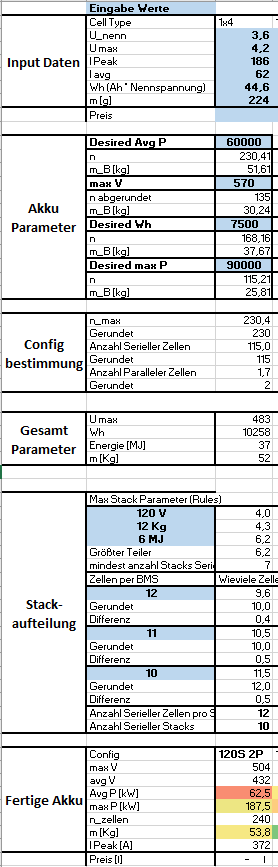
\includegraphics[width=0.2\linewidth]{bilder/Ausschnitt_zellvergleich}
	\caption{Ausschnitt aus der Zellauswahl Excel}
	\label{fig:Ausschnitt_zellvergleich}
\end{figure}

Unter dem Punkt Input Daten werden die Zellparameter aus dem Datenblatt der Zelle angegeben. Unter den Akkuparametern werden nun die Zielbedingungen bzw., Grenzwerte für den Akku bestimmt. Die min Avg. P. ist hierbei ein Parameter für die im Endurance angestrebte Leistung, die max.V ergibt sich aus der Spannungsfestigkeit des \ac{TS}, besonders relevant sind hierbei die Elektromotoren. Die min. Wh geben die mindestens vorgesehene Akkukapazität vor und die min. max. P. die angestrebte maximale Leistung die der Akku leisten muss. Aus diesen Parametern wird folgend eine minimal benötigte Zellanzahl bestimmt. Unter dem Punkt Akkuconfig wird nun die vorherig höchste bestimmte Zellanzahl ermittelt und gerundet. Hieraus bestimmen wir nun die Anzahl der parallel und seriell verschalteten Zellen und runden auf ganze Zellen.\\
Dies ergibt dann einige Gesamtparameter für den Akku.\\
Unter dem Abschnitt Stackaufteilung werden die Zellen jetzt nach den Parametern des Regelwerkes möglichst optimal in Stacks aufgeteilt. Der Zielwert hierbei ist es, dass die tatsächliche Anzahl an Akkuzellen größer ist als die vorher errechnete benötigte Anzahl, es wird also aufgerundet. Weiter soll möglichst eine gerade Anzahl an Stacks herauskommen so das sich die Stacks im Akku möglichst leicht verteilen lassen. Hierbei können wir drei verschiedene Anzahlen von Zellen pro \ac{AMS} vorgeben die analysiert werden sollen.\\
Schlussendlich ist das Ergebnis ein fertig konfigurierter Akku. Diese Konfigurationen können nun gegenübergestellt und die Anzahl der weiter zu analysierenden Zellen eingegrenzt werden.\\
\\
Zur weiteren Analyse wurde auf folgende aufbereitete Messdaten zurückgegriffen. Die Datengrundlage stammt von den Tests zweier Webseiten \cite{dampfakkusVTC6,lygteVTC6}.

\begin{figure}[h]
	\centering
	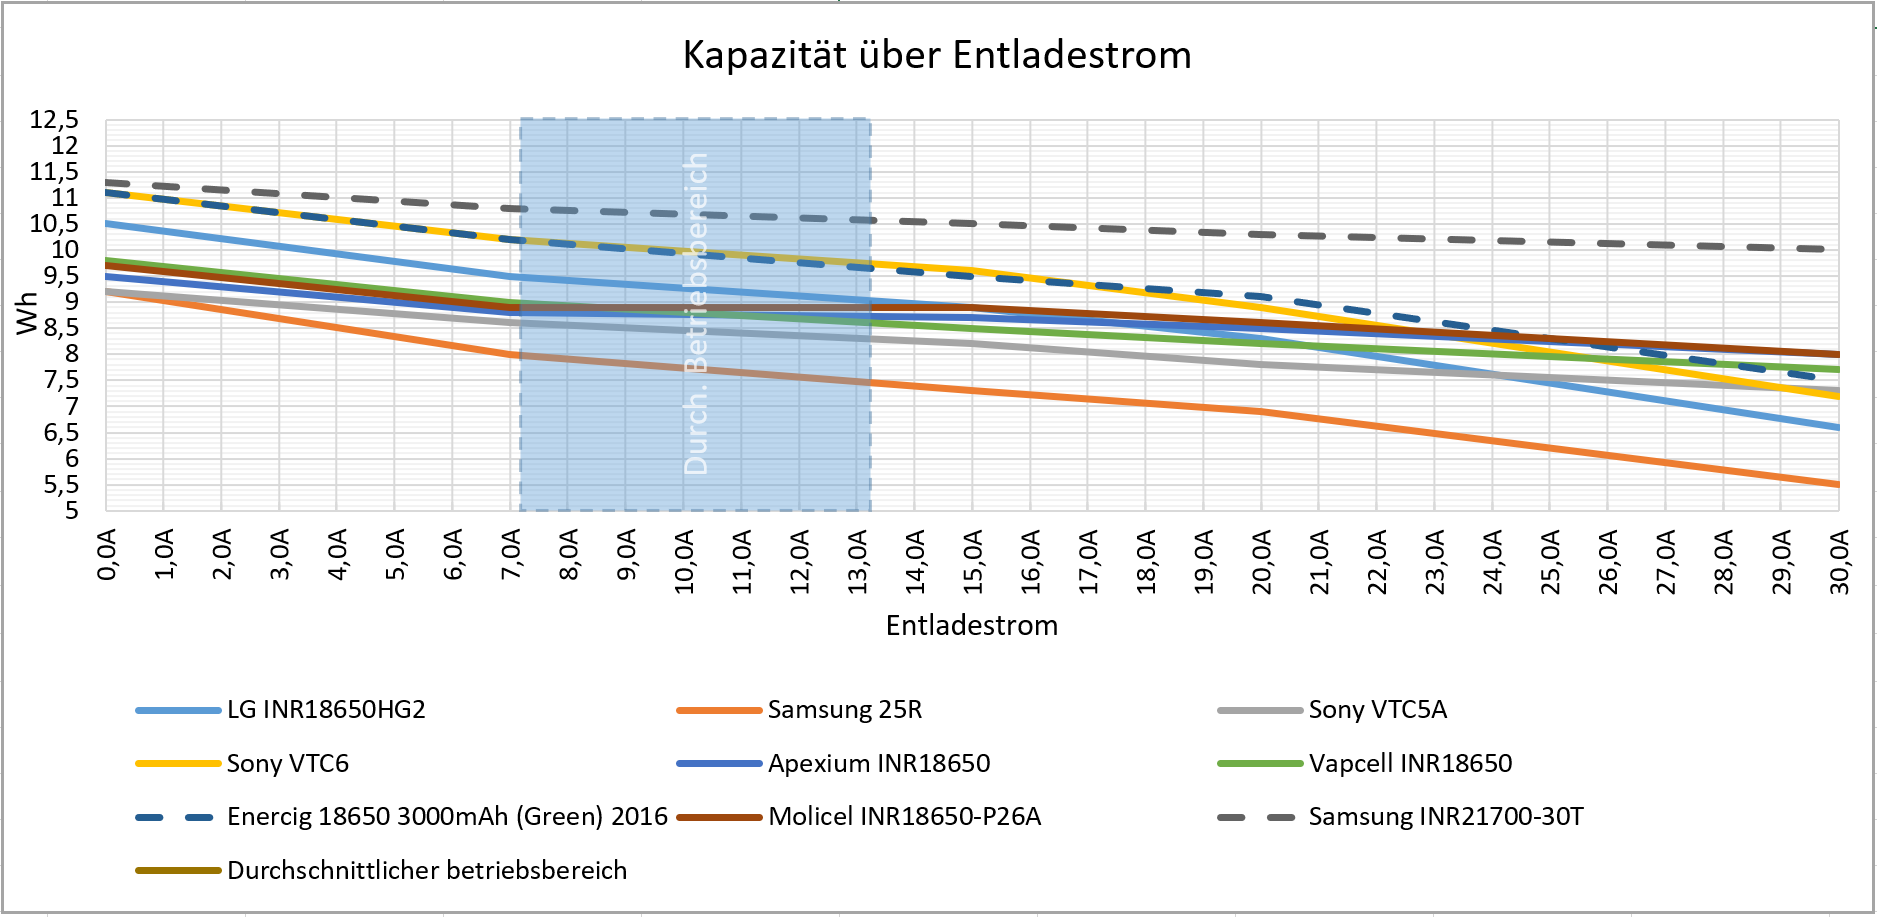
\includegraphics[width=0.6\linewidth]{bilder/Kapazitaet_ueber_Entladestrom}
	\caption{Kapazität über Entladestrom}
	\label{fig:Kapazitaet_ueber_Entladestrom}
\end{figure}

\begin{figure}[h]
	\centering
	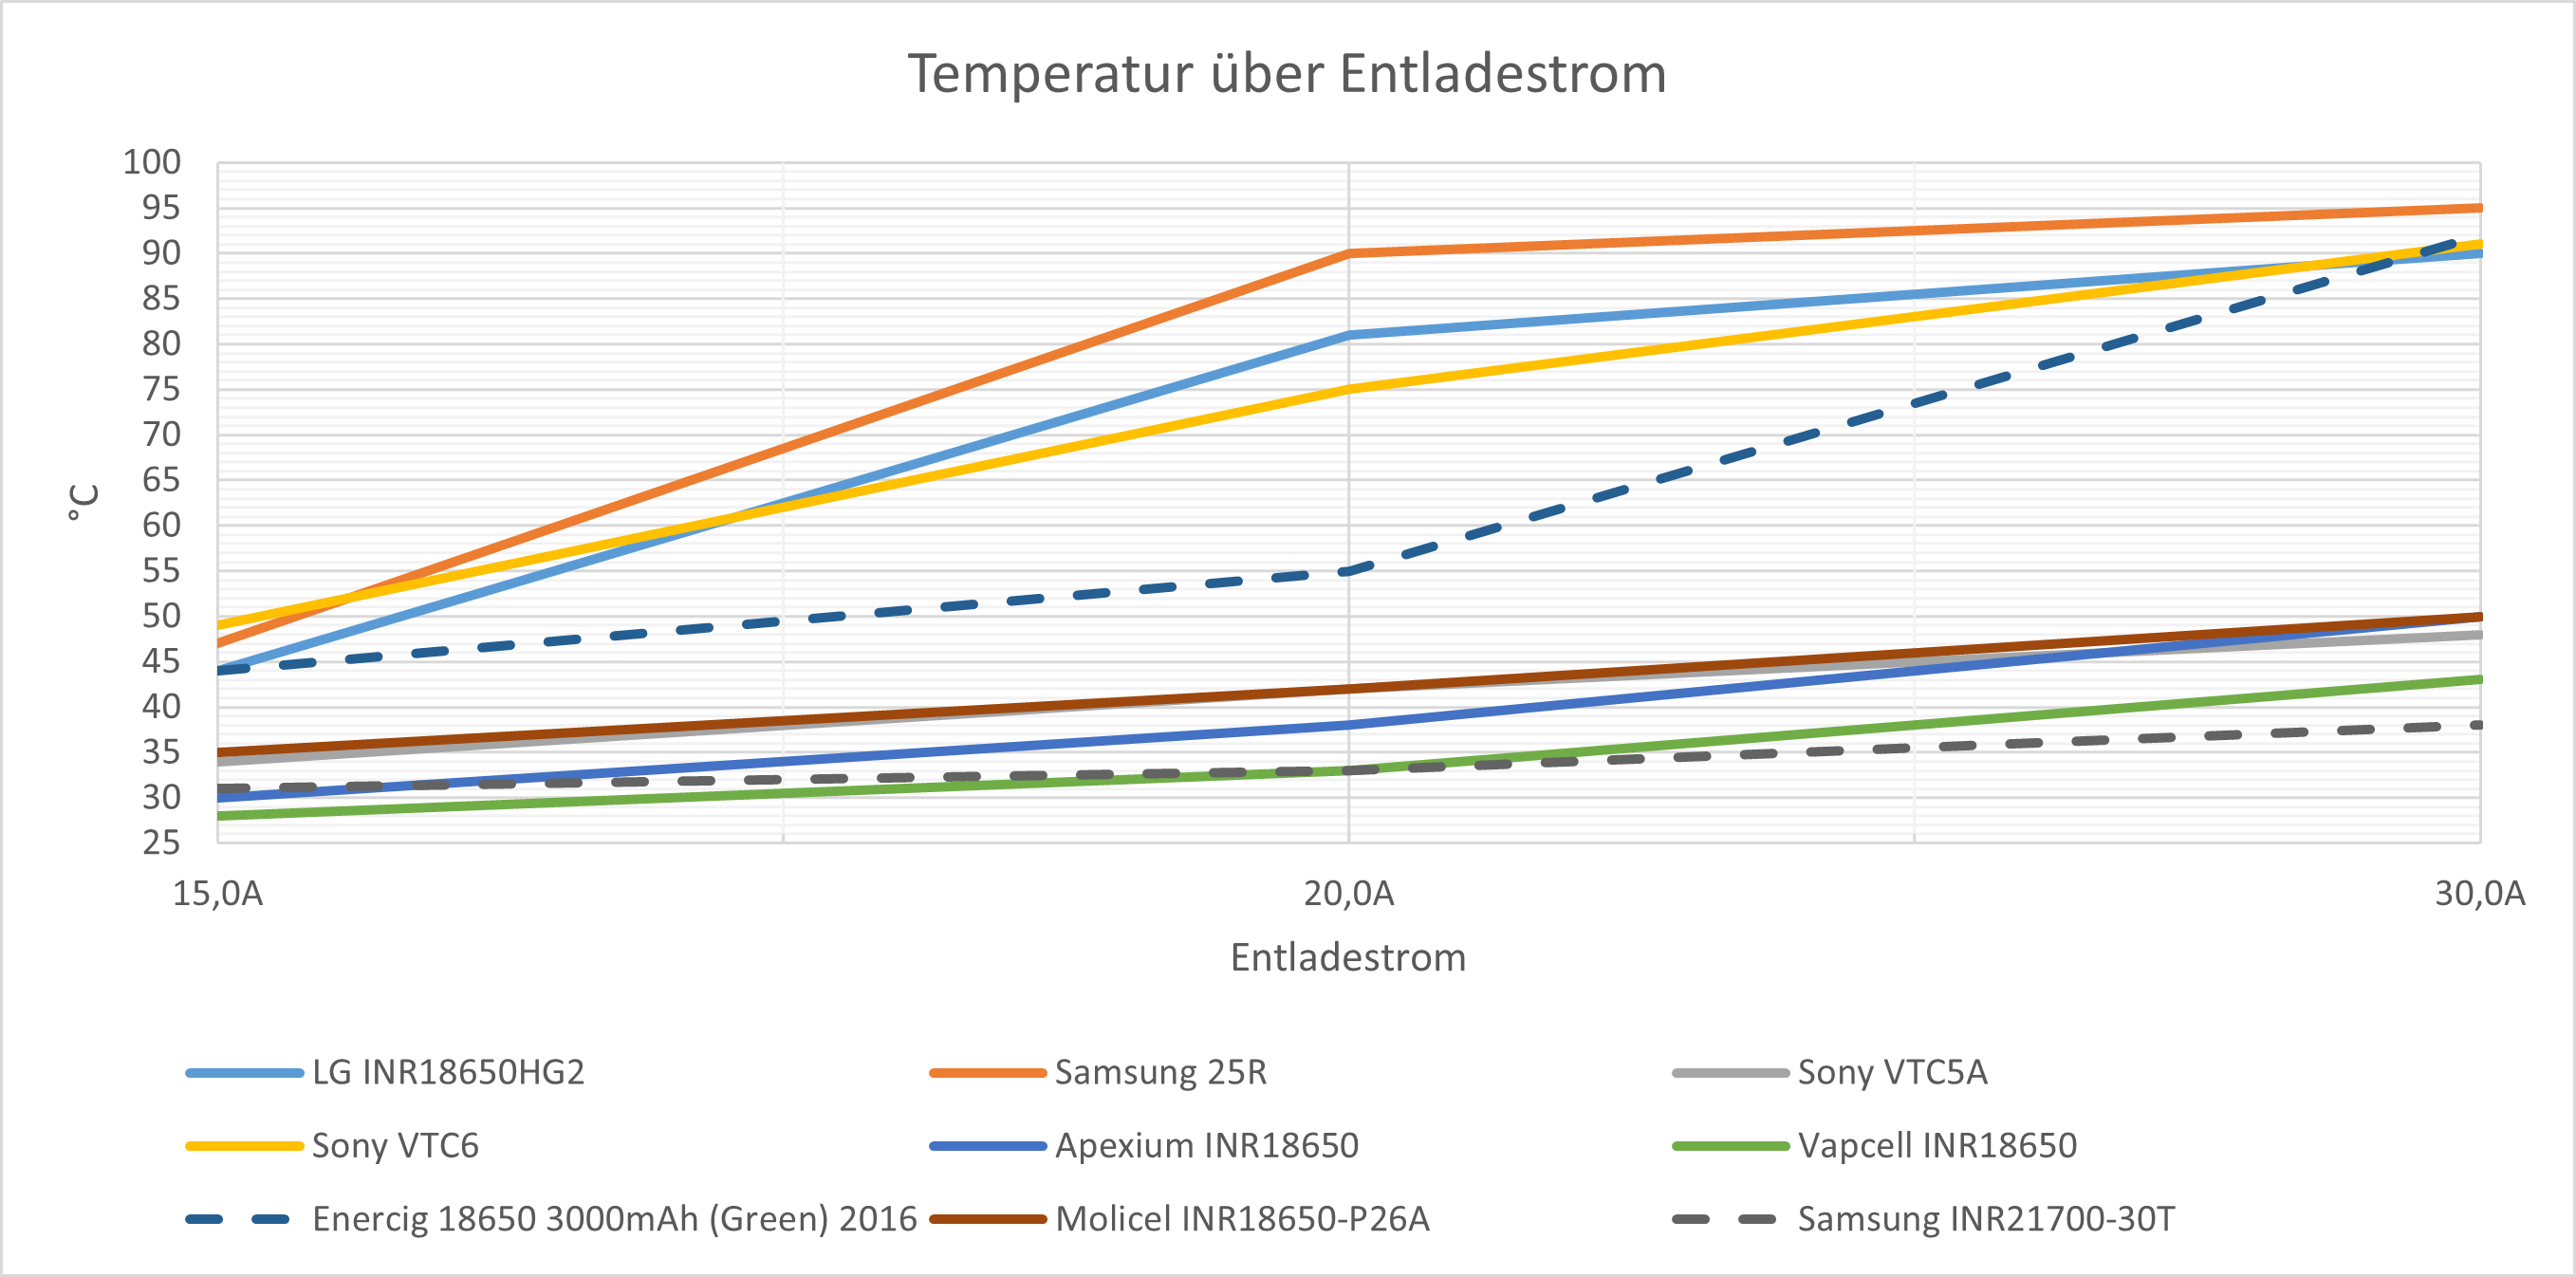
\includegraphics[width=0.6\linewidth]{bilder/Temperatur_ueber_Entladestrom}
	\caption{Temperatur über Entladestrom}
	\label{fig:Temperatur_ueber_Entladestrom}
\end{figure}

Das erste Diagramm ermöglicht es einen Eindruck von der Entladeeffizienz des Akkus, besonders bei hohen Strömen zu bekommen. Das Optimum wäre hier eine Horizontale Linie am oberen Rand des Diagramms. Hierbei sticht die Samsung INR21700-30T besonders hervor.\\
Das zweite Diagramm ermöglicht uns einen Eindruck von der thermischen Performance zu erlangen. Laut Regelwerk der Formula Student darf keine Akkuzelle zu einem Zeitpunkt die \ensuremath{60°C} Marke überschreiten. Nichtbeachten führt zur Disqualifikation. hierbei sticht auch die vorher genannte Samsung Zelle hervor als auch die Vapcell INR18650\\
Hierbei vergleichen wir Rundzellen von verschiedenen Baumaßen, ein Vollständiger Akku mit den Samsung INR21700-30T wäre \ensuremath{7Kg} schwerer als einer mit der Sony VTC6. Daher müssen am Ende alle erlangenden Erkenntnisse Berücksichtigt werden.

%evtl. netzgrafik von den top 2 oder 3 zellen machen. als finale gegenüberstellung 
\FloatBarrier
\subsubsection{Elektrisches Modell der Zelle}
Das Elektrische Modell ist für die Modellierung in der \ac{LTS} relevant. Hierbei werden die Limitierungen die sich aus dem Akku und dem restlichen Antriebsstrang ergeben simuliert. Ein Beispiel ist die sinkende Antriebsleistung bei abfallen der Spannung durch sinkenden \acfirst{SOC}. Das aktuelle Modell greift dabei auf zwei Datensätze zu um das verhalten zu modellieren. Einmal die Entladeeffizienz bzw. einen korrigierten Entladestrom, als auch auf ein Spannungskennfeld über den Entladestrom und \ac{SOC}. Die folgenden Abbildungen \ref{fig:Entladeeffizienz_VTC6} und \ref{fig:Spannung_ueber_SOC_Strom} gelten für die Sony VTC6. Die Daten entstammen wieder der Webseiten dampfakkus.de und lygte-info.dk.
\begin{figure}[h]
	\centering
	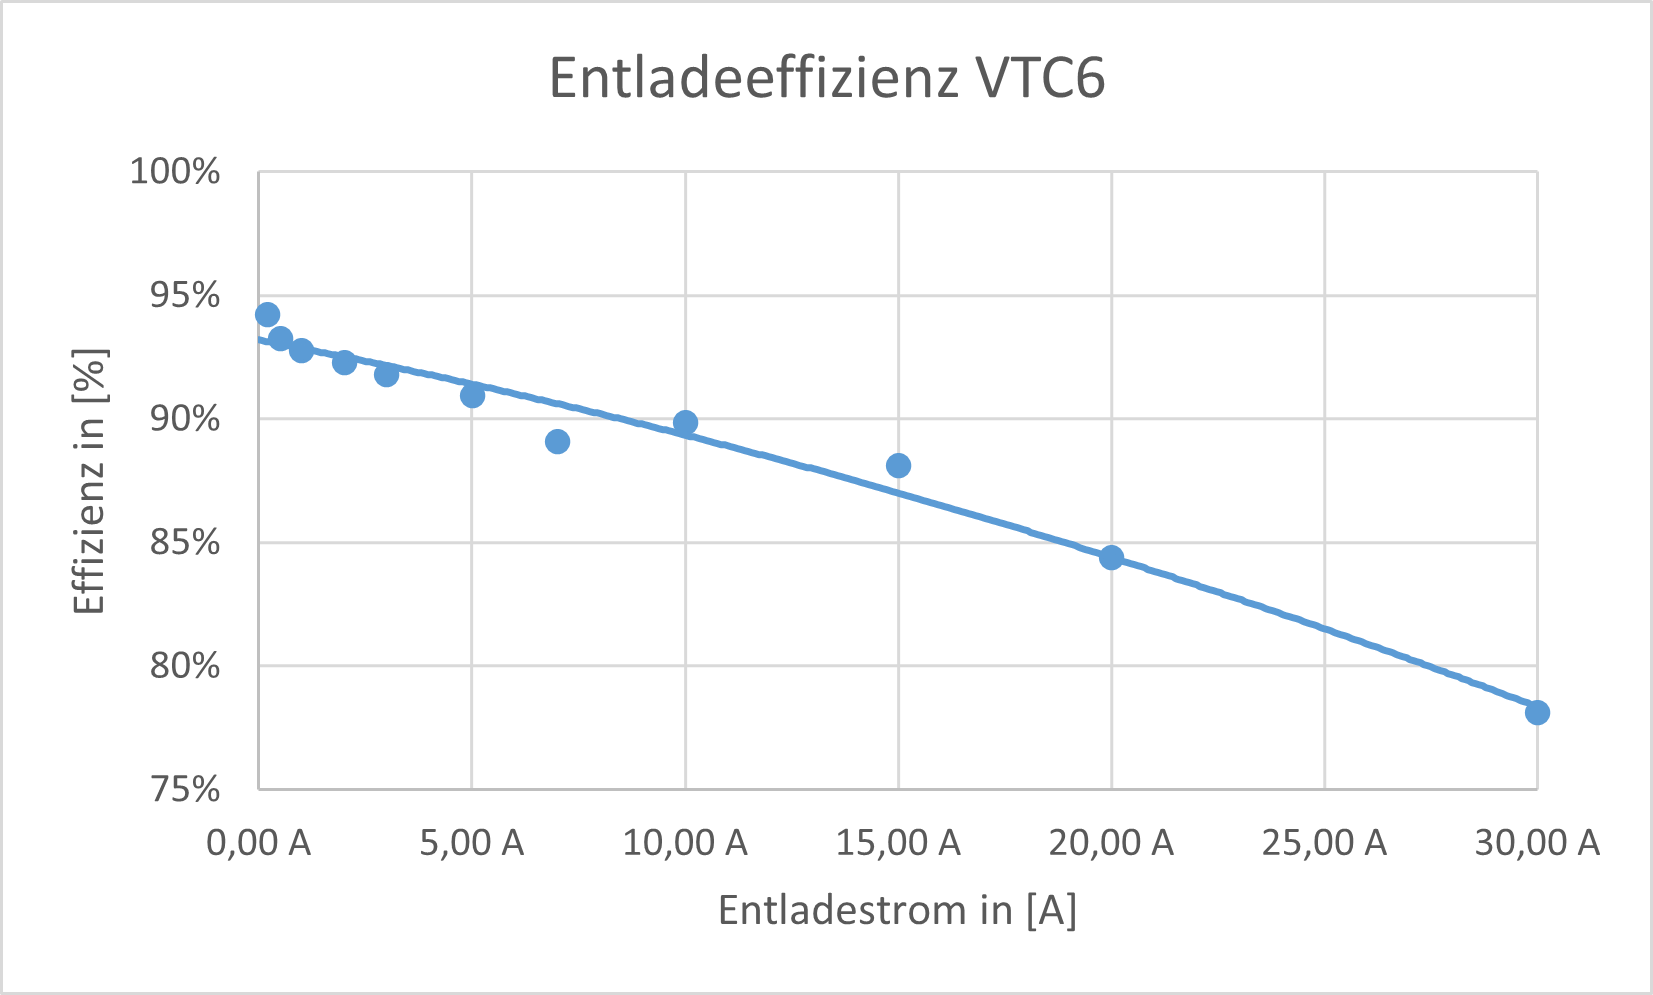
\includegraphics[width=0.7\linewidth]{bilder/Entladeeffizienz_VTC6}
	\caption{Entladeeffizienz VTC6}
	\label{fig:Entladeeffizienz_VTC6}
\end{figure}
\begin{figure}[h]
	\centering
	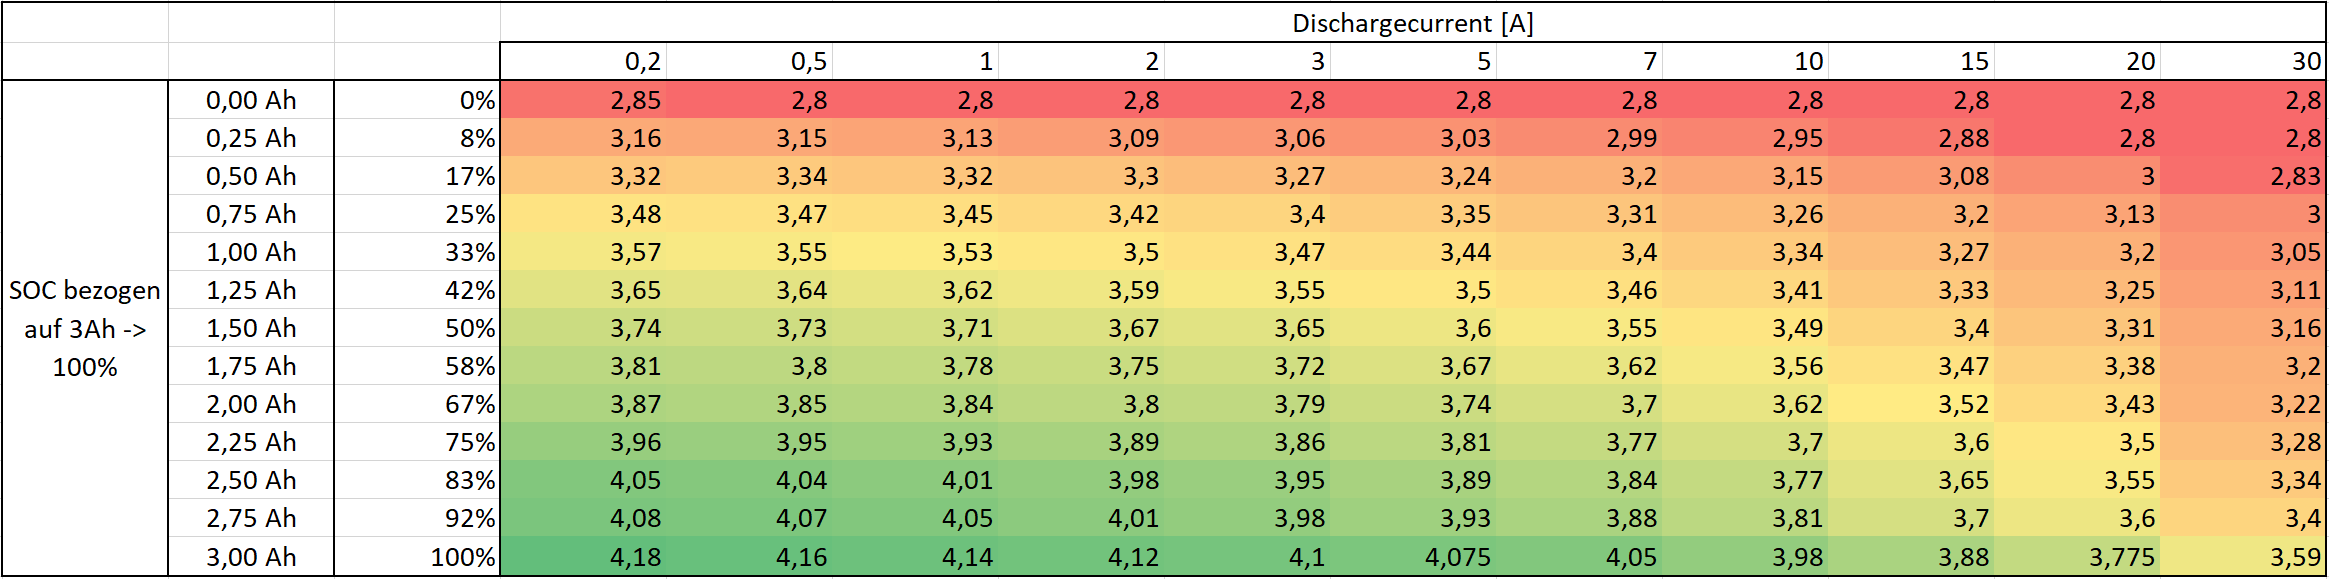
\includegraphics[width=0.7\linewidth]{bilder/Spannung_ueber_SOC_Strom}
	\caption{Spannungskennfeld VTC6}
	\label{fig:Spannung_ueber_SOC_Strom}
\end{figure}
\FloatBarrier
\subsubsection{Temperaturmodell der Zelle}
%Quelle!!!
Auf Basis der in Abbildung \ref{fig:parameterthermischesmodellvtc6} dargestellten Parameter  können wir ein analytisches thermisches Modell der Akkuzelle erstellen. Bei der Ermittlung dieser wurde unter anderem die Akkuzellen des Typs VTC6 innerhalb einer Thermal Vakuum Kammer betrieben.

\begin{figure}[h]
	\centering
	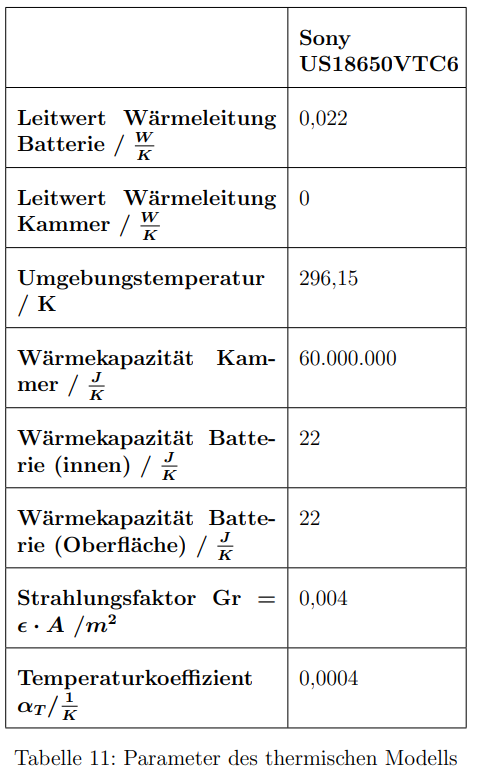
\includegraphics[width=0.4\linewidth]{bilder/Parameter_thermisches_modell_VTC6}
	\caption{Parameter des thermischen Modells der VTC6 \cite{Klein2017}}
	\label{fig:parameterthermischesmodellvtc6}
\end{figure}

Damit ergibt sich folgende Gleichung.

\begin{equation}
	\glsc{symb:T_celli+1} = (\glsc{symb:I_cell}^2 * \glsc{symb:R_cell} - \glsc{symb:G_th} * (\glsc{symb:T_celli} - \glsc{symb:T_u}) - \glsc{symb:G_r} * \glsc{symb:SBoltz} * (\glsc{symb:T_celli} - \glsc{symb:T_u})^4) * \dfrac{1}{\glsc{symb:C_B} * \glsc{symb:m_Cell}} + \glsc{symb:T_celli}
\end{equation}

Mit dieser Gleichung ergeben sich folgende Kurvenverläufe für eine Auswahl von Entladeströmen.

\begin{figure}[h]
	\centering
	\includegraphics[width=0.7\linewidth]{bilder/temperatur_über_energie_vtc6_thermo_modell}
	\caption{Temperatur über Energieverbrauch VTC6}
	\label{fig:temperaturuberenergievtc6thermomodell}
\end{figure}
%Quelle
Mithilfe der Grafik \ref{fig:messdatenvtc6-temperatur-kapazitat-spannung} können wir einen Plausibilitätscheck durchführen. Wir haben hier Messdaten von der Sony VTC6. Hierbei sind jedoch die Testbedingungen unbekannt.

\begin{figure}[h]
	\centering
	\includegraphics[width=0.7\linewidth]{"bilder/Messdaten_VTC6_ temperatur kapazität spannung"}
	\caption{Messdaten Temperatur über Energieverbrauch \cite{Hnidka2020}}
	\label{fig:messdatenvtc6-temperatur-kapazitat-spannung}
\end{figure}

Wir sehen, dass das erstellte Modell für den \ensuremath{10 A} Graphen um ca. \ensuremath{3°C} abweicht. Weiterhin sehen wir das bei der \ensuremath{20 A} Linie die \ensuremath{90°C} ca. \ensuremath{0,5 Ah} früher erreichen. Diese Abweichungen sind nicht insignifikant, zeigen jedoch das unser Modell eher zu hohe als zu niedrige Temperaturen ausgibt was für die Zuverlässigkeit des Fahrzeuges positiv ist, da eine Auslegung der Kühlung mit diesem Modell wahrscheinlich zu einer Überkühlung und damit zu einem zu hohen Gewicht des Kühlsystems führt was für das erste Fahrzeug kein sonderlich großes Problem darstellt. Die Abweichung dürfte darauf zurückzuführen sein das die Modellparameter im Vakuum ermittelt wurden und insofern Wärmeübertragung durch Konvektion etc. nicht berücksichtigt werden konnte. Um diesem Sachverhalt weiter auf den Grund zu gehen wurde im Anschluss eine Simulation mit Ansys Fluent durchgeführt.

\begin{figure}[h]
	\centering
	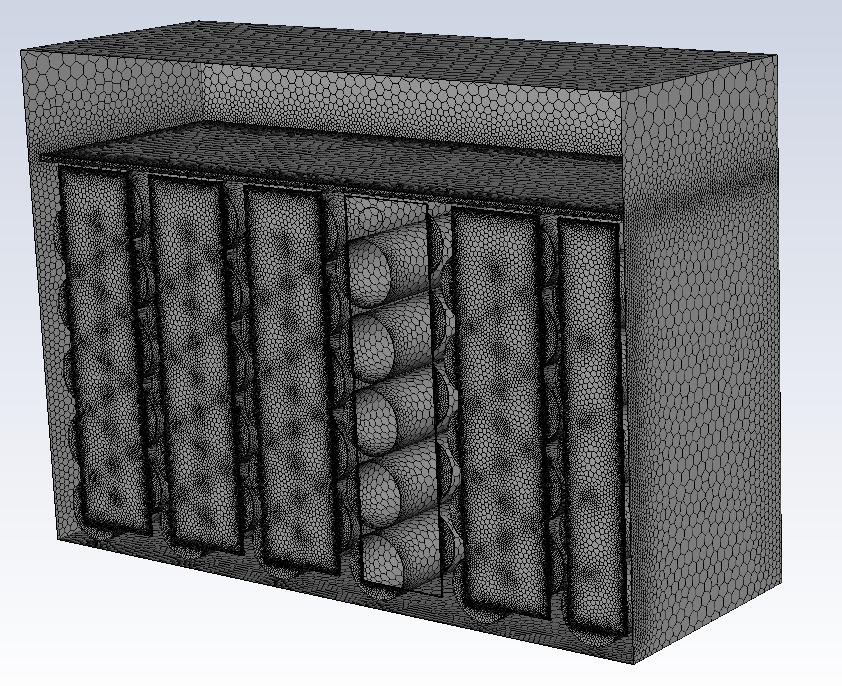
\includegraphics[width=0.7\linewidth]{bilder/Accu_Sim_therm_7_2A_45min_simple_mesh}
	\caption{Mesh der Multiphysik Fluent Simulation des Akkustacks}
	\label{fig:accusimtherm72a45minsimplemesh}
\end{figure}

\begin{figure}[h]
	\centering
	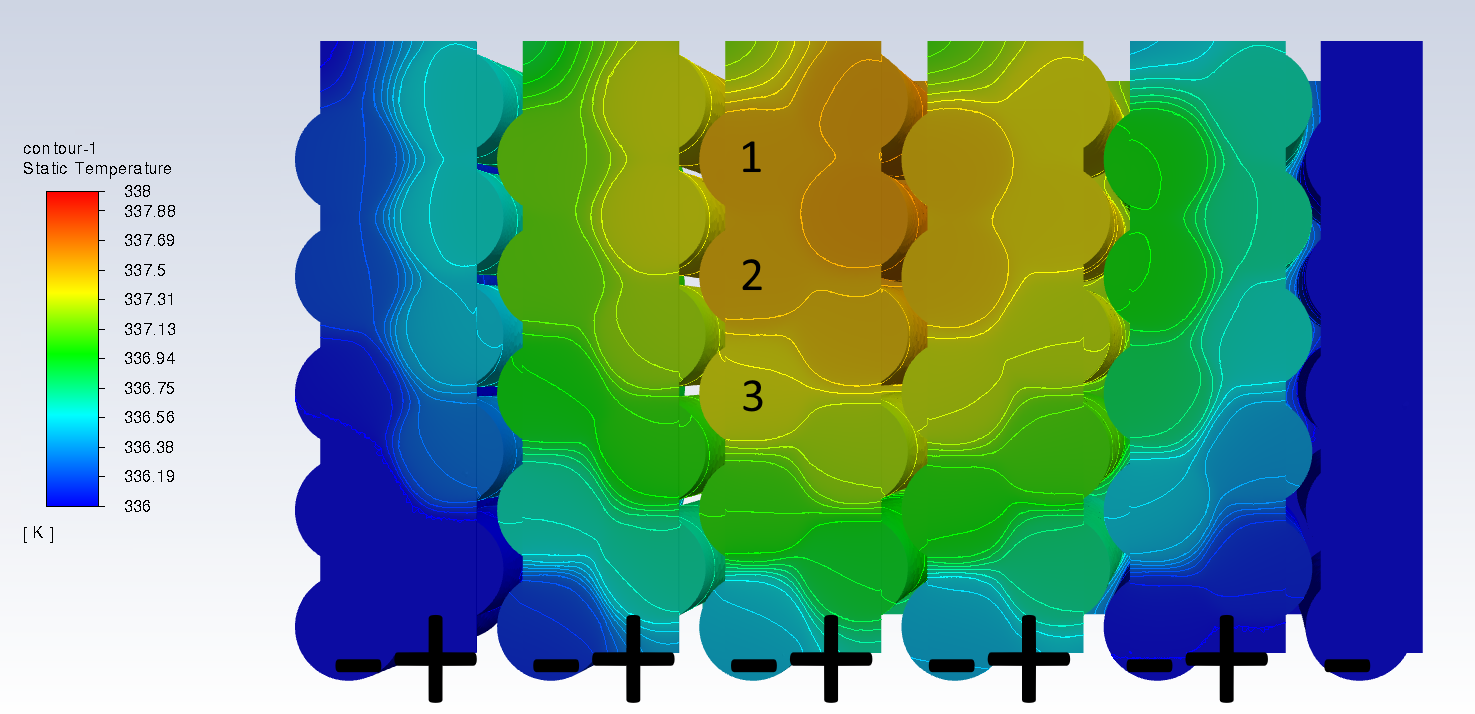
\includegraphics[width=0.7\linewidth]{bilder/Accu_Sim_therm_7_2A_45min_simple}
	\caption{Multiphysik Simulationsergebnis Akkustack}
	\label{fig:accusimtherm72a45minsimple}
\end{figure}

In dieser Simulation wurde ein gesamter Akkustack in seinem Gehäuse simuliert. Dabei wurde mit einem konstanten Strom von \ensuremath{7,2 A} simuliert. Dieser Strom ergibt sich aus der \ac{LTS}. Die Simulation wurde für \ensuremath{32 min} laufen gelassen um ein gesamtes Endurance darzustellen. Ziel der Simulation ist es die Effekte der Konvektion zu berücksichtigen, aber auch zu sehen inwiefern sich die Zellen gegenseitig beeinflussen. Allerdings wurden auch diverse Vereinfachungen getroffen insofern das die Akkuzellen sich uniform aufwärmen. In der Realität dürfte man am negativen Pol der Akkuzelle eine deutlich höhere Temperatur feststellen können als auf der positiven Seite. Weiterhin wurden diverse Teile wie die elektrische Isolierung etc. weggelassen da dies den Simulationsaufwand sonst erheblich vergrößert hätte. Mit den vorliegenden Vereinfachungen lief die Simulation für 46 Stunden.\\
Zur Analyse, wir sehen nach der Simulationszeit eine Höchsttemperatur von \ensuremath{64,85°C} und eine Tiefsttemperatur von \ensuremath{62,85°C}. In dieser Hinsicht stimmt die Ansys Simulation eher mit der \ensuremath{10 A} kurve aus unserem Modell zusammen als mit den Messdaten. Zusammengefasst stellt man fest das definitiv weitere Arbeit in diesem Themenbereich von Nöten wäre, um zu einer optimalen Lösung zu kommen, dies jedoch aufgrund des engen Zeitplanes und des enormen anderweitigen Aufwandes nicht möglich ist.

\FloatBarrier
\subsection{Der Stack Aufbau} %(mit Tim)%

Für die Konstruktion des Akkustacks gab es im Laufe der Saison viele Iterationen. Die folgend erläuterte ist eine Optimierte Version derer die für den TY22 gebaut wurde.

\begin{figure}
	\centering
	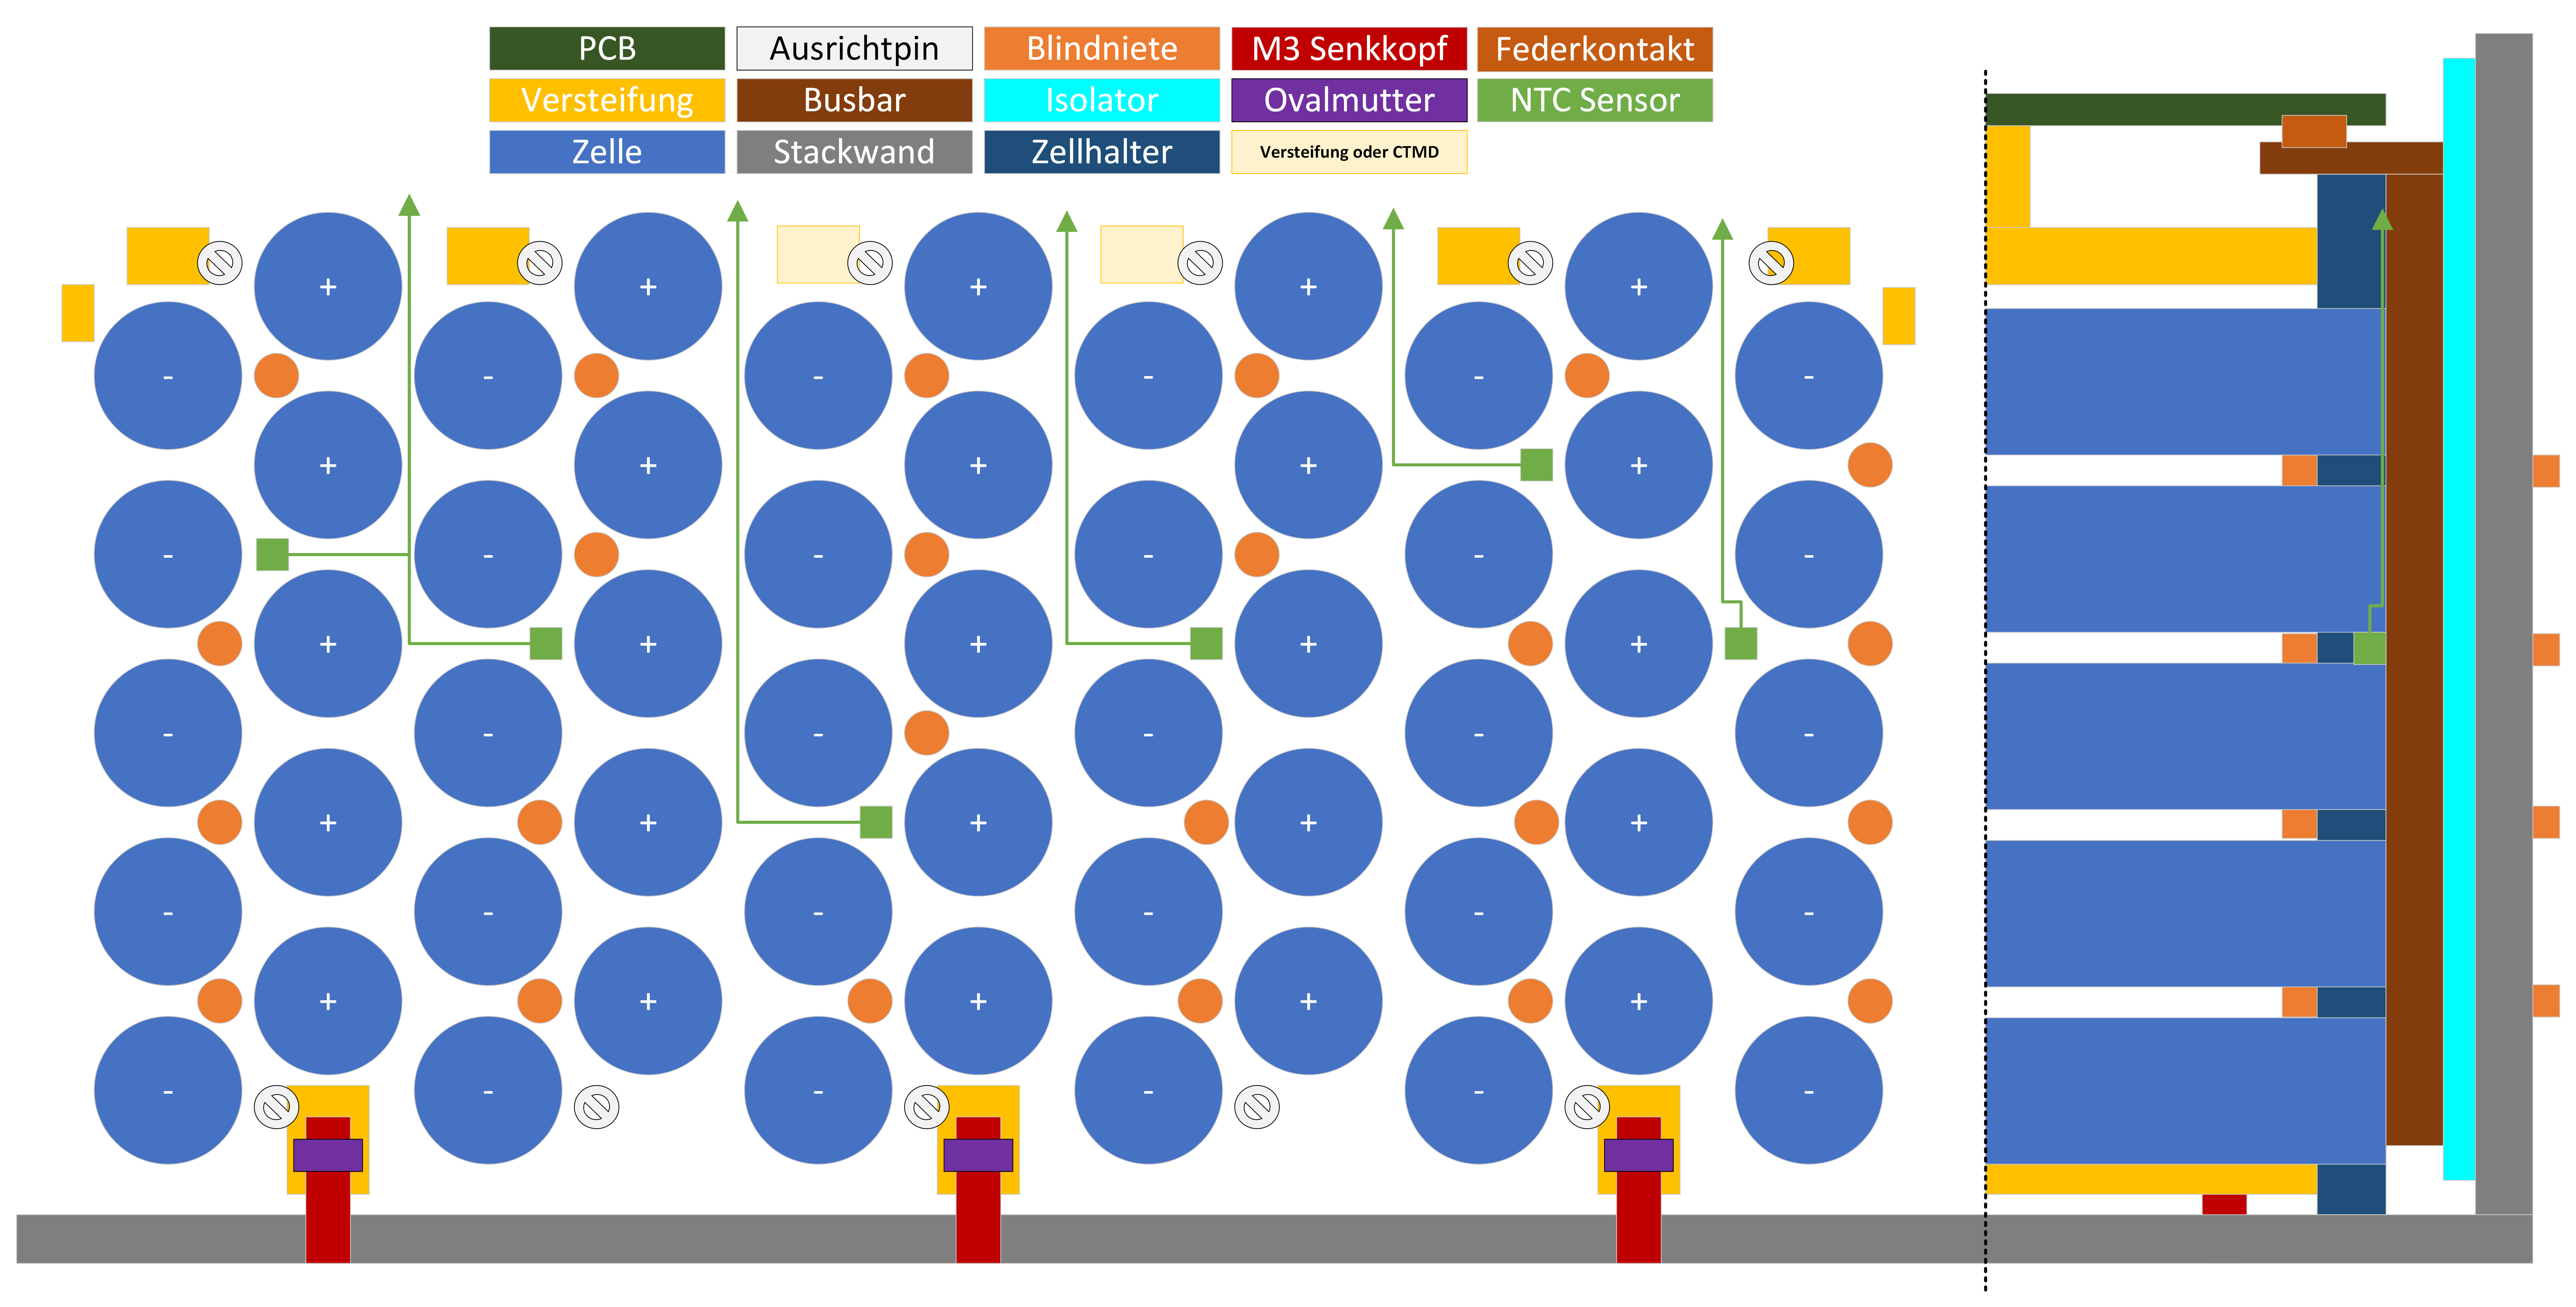
\includegraphics[width=0.7\linewidth]{bilder/Stackaufbau_Prinzipskizze}
	\caption{Prinzipskizze Stackaufbau}
	\label{fig:stackaufbauprinzipskizze}
\end{figure}

\begin{figure}
	\centering
	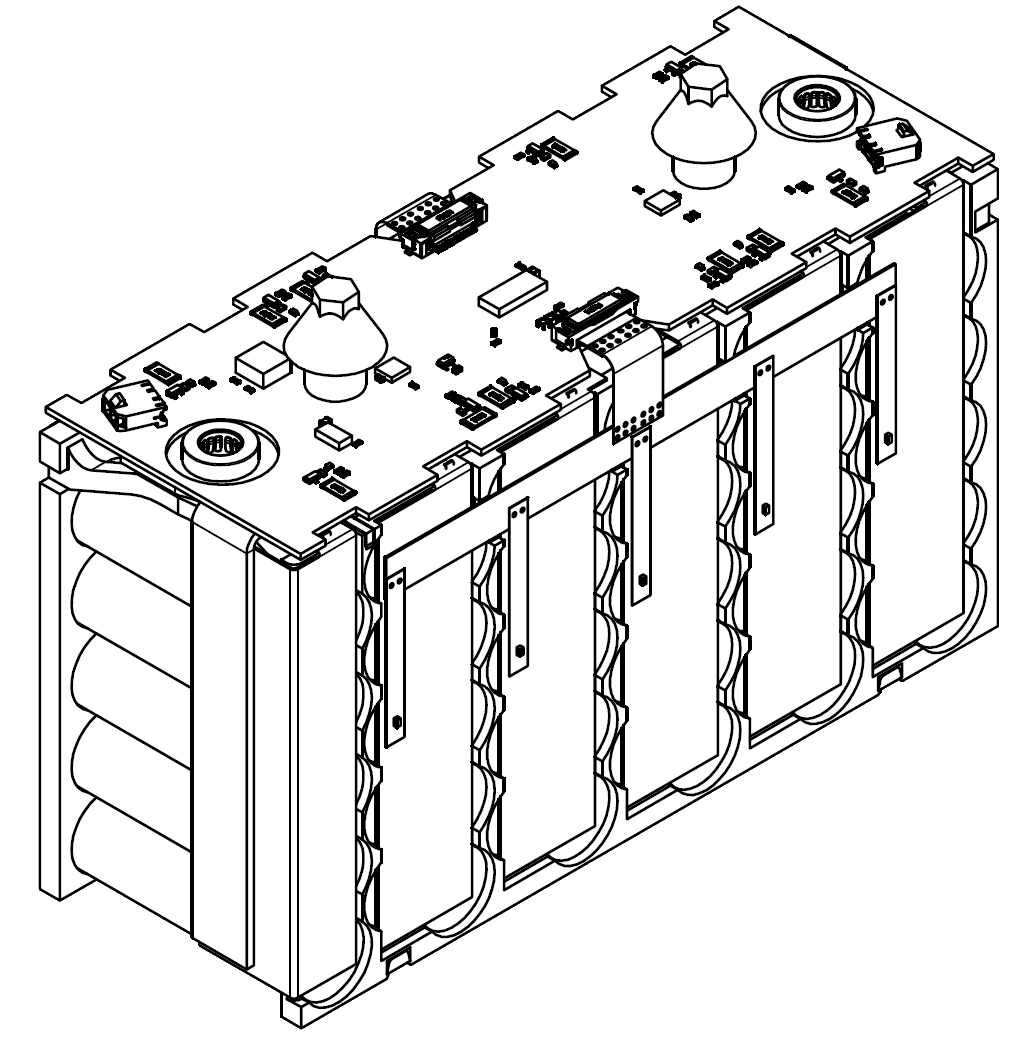
\includegraphics[width=0.7\linewidth]{bilder/Stach_for_EDR}
	\caption{Iso Ansicht Stack Baugruppe}
	\label{fig:stachforedr}
\end{figure}

Die Zellen sind liegend in Fünferpaketen gestapelt und mit einem Versatz aneinander gereiht um den Leerraum zwischen den Zellen möglichst klein zu halten. Die Busbars verbinden immer ein 5er Negativpole mit einem 5er positiv Pole. Zusätzlich befinden sich in der nähe der Zellen 2 Ausrichtpins um die Busbar auf dem Stack bei der Montage positionieren zu können. Der Aufbau auf den Polen besteht aus einer angeschweißten Busbar, darauf folgt ein abriebfester Isolator, und dann die Trennwand des Akkus. nach Innen haben wir noch einen 3D gedruckten Halter in dem die Akkuzellen ausgerichtet werden. Dieses ganze Paket wird mit Blindnieten vernietet. Ziel hierbei ist es einen möglichst guten thermischen Kontakt von den Polen der Zelle zum Akkugehäuse herzustellen. Selbiges ist aus Aluminium und Flächig mit dem Monocoque verschraubt welches auch aus Aluminium gefertigt ist. dies ergibt eine riesige thermische Masse und stellt so eine Kühlung für den Akku bereit. Die Stack-Seitenwand liegt als L-Profil vor, und wird anschließend mit dem Akkuboden mit Hilfe von M3 Senkkopfschrauben und Ovalmuttern verschraubt. In diesem Zuge sind in die 3D gedruckten Querversteifungen im Stack Ovalmuttern eingeklebt. Diese Querversteifung sorgen einerseits für mechanische Stabilität, stellen aber auch Anbindungspunkte für den \ac{AMS}-Slave als auch für die Maintenance Plug Steckverbinder bereit. Die Busbar ist auch als L-Profil ausgeführt und lappt oben über den Stack über, diese Finnen werden seitens des \ac{AMS}-Slaves mit Hilfe von Federkontakten kontaktiert um eine Verbindung für die Spannungsmessung als auch das Balancing herzustellen. Die \acfirst{NTC}-Sensoren befinden sich in den Leerstellen wo keine Nieten benötigt werden, immer eine Niete mittig in drei Zellen. Die \ac{NTC}`s sind rückseitig auf die Busbar geklebt. Um das Design günstig zu halten kann die Verbindung über \ensuremath{0,25mm^2} Kabel erfolgen, welche Sensorseitig auf Lötpads und \ac{AMS}-seitig in einen Stecker gebracht werden. Bei der Steckverbinderauswahl ist zu beachten das er über einen Verriegelungsmechanismus verfügt, und nicht zu klein ist. Besonders kleine Steckverbinder machen an der stelle die Verarbeitung schwer oder praktisch unmöglich. Präferiert wäre hier ein Flex-\acfirst{PCB}, dies ist jedoch \ac{idR} recht teuer. In dem Stackhalter müssen entsprechende Einkerbungen vorgehalten werden durch die die Kabel zu führen sind. In die Anbindung des \ac{AMS}-Slave ist ein Feature vorzusehen welches eine leichte Extraktion des Stacks aus dem Akku erlaubt, und bei der Konstruktion der Maintenance Plugs ist auf Ergonomie zu achten, so das ein Mensch mit einem \ac{HV}-Handschuh noch gefahrlos einen solchen ziehen kann. Weiter ist bei den Maintenance Plugs auf Verstecksicherheit zu achten. Ein letzter Punkt ist die Positionierung des \acfirst{CTMD}, also entweder des i-Button oder der kabelgebunden Sensoren mit Steuergerät, je nachdem was die \acfirst{FSG} verwenden möge. Hier ist besonders die Positionierung des \ac{CTMD} am Hotspot schwer nachzuweisen. Eine Simulation kann hier eine Richtung aufzeigen, stellt jedoch einen großen Zeitaufwand dar und ist im allgemeinen so ungenau (ohne signifikanten Zeitaufwand), dass sich nur sehr begrenzt belastbare Aussagen hiermit treffen lassen.

\FloatBarrier
\subsection{Die Busbar}
 Bei der Auswahl der Materialien für die Busbar sind die Masse als auch die elektrische, respektive die thermische Performance ausschlaggebend. Ein weiterer Maßgebender Faktor sind die möglichen Fertigungsverfahren um den Kontakt zwischen Zelle und Busbar herzustellen. Folgende Grafiken ergeben sich aus den Materialkonstanten und der Erwärmung über den Widerstand der Busbar bei dem entsprechenden Strom und über die Wärmekapazität und die Betriebszeit.
 
 \begin{figure}[]
 	\centering
 	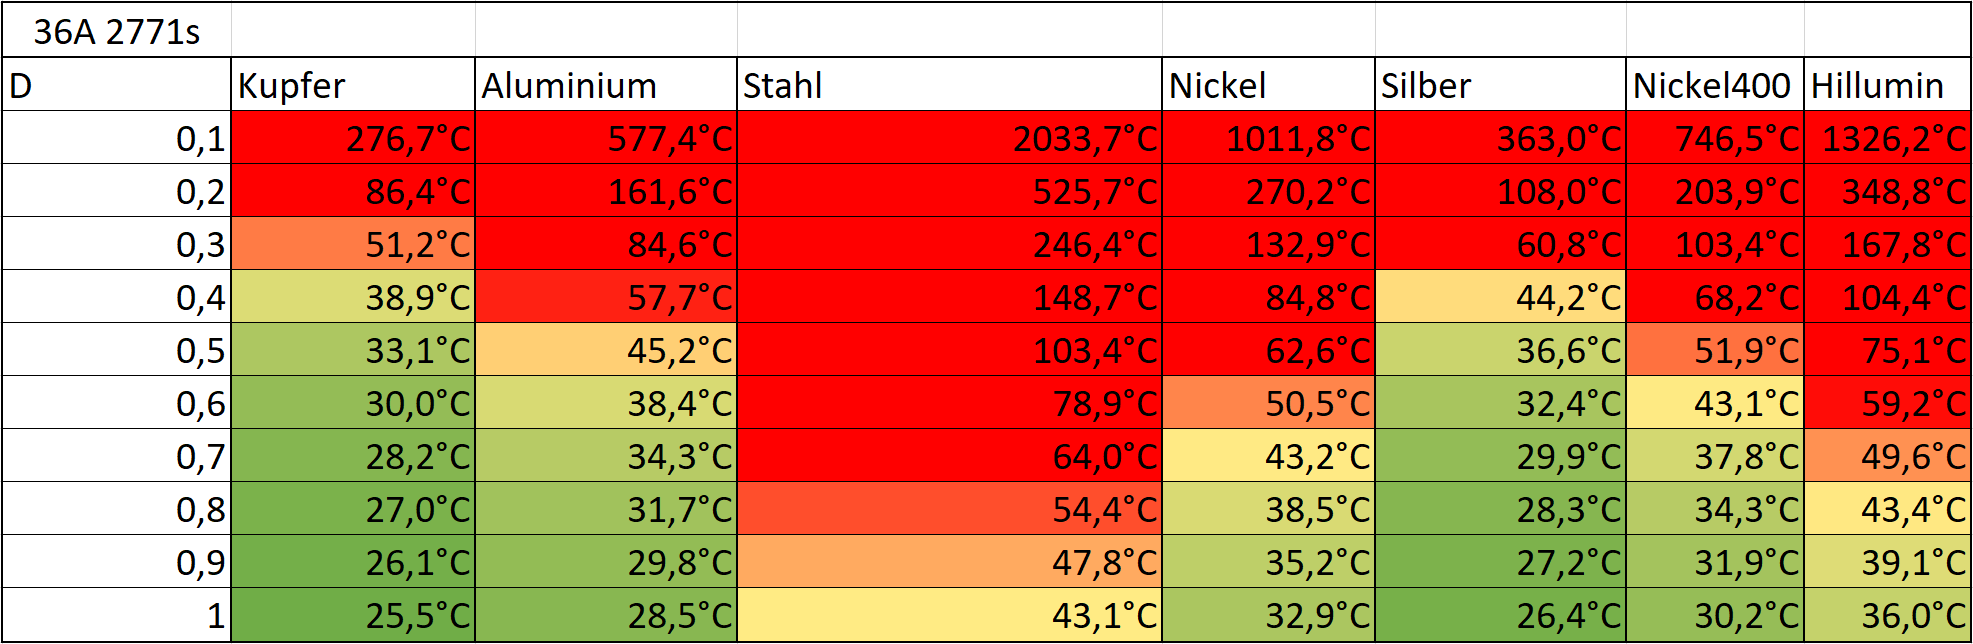
\includegraphics[width=0.7\linewidth]{bilder/Busbar_temp_36A_2771s}
 	\caption{Busbartemperatur bei 36 A und 2771 s}
 	\label{fig:Busbar_temp_36A_2771s}
 \end{figure}
\begin{figure}[]
	\centering
	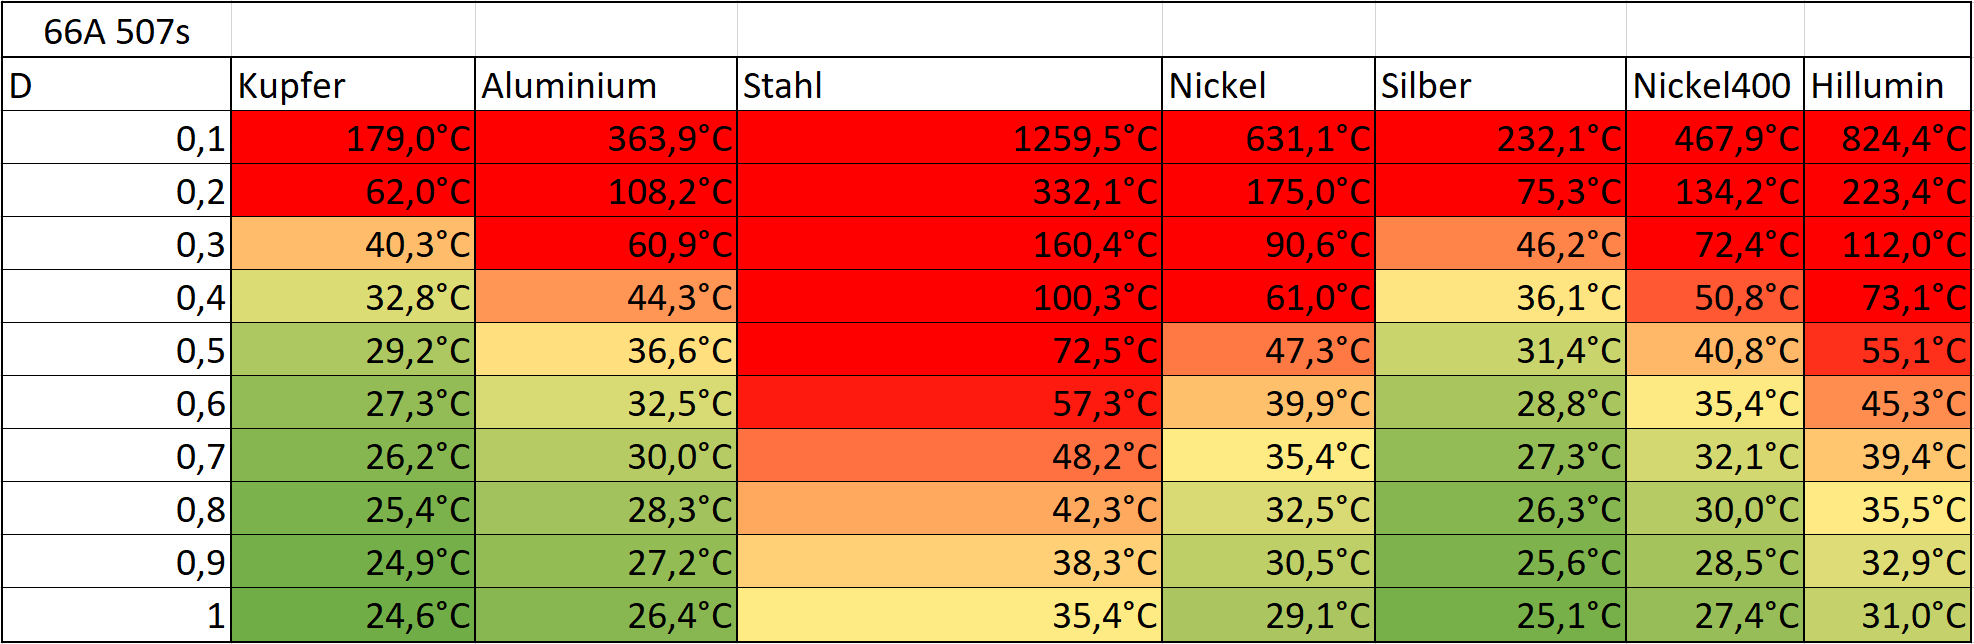
\includegraphics[width=0.7\linewidth]{bilder/Busbar_temp_66A_507s}
	\caption{Busbartemperatur bei 66 A und 507 s}
	\label{fig:Busbar_temp_66A_507s}
\end{figure}
\begin{figure}[]
	\centering
	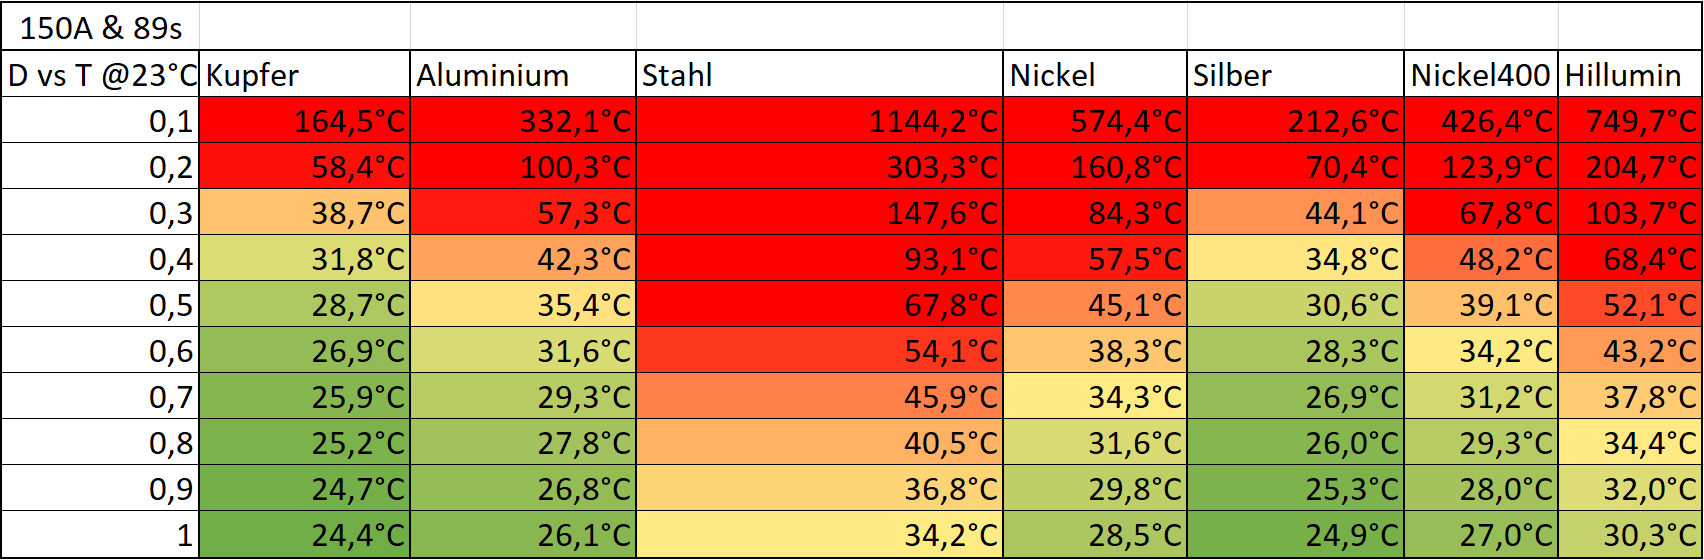
\includegraphics[width=0.7\linewidth]{bilder/Busbar_temp_150A_89s}
	\caption{Busbartemperatur bei 150 A und 89 s}
	\label{fig:Busbar_temp_150A_89s}
\end{figure}

Es ist ersichtlich das Kupfer die beste thermische Performance in Bezug auf die Materialmenge bringt, aufgrund der niedrigen dichte Aluminium allerdings gravimetrisch mit Abstand die beste Performance zeigt. Nickel, respektive Nickel 400 liegen jedoch nicht weit zurück, lediglich stahl lässt sich aufgrund der Ergebnisse direkt ausschließen.\\
\\
In Bezug auf die Fertigung ergeben sich bei Rundzellen zwei Wege, einmal das Schweißen aber auch die Federkontaktierung.\\
Die Kontaktierung über eine Feder an eine Rundzelle sollte dem Leser hinreichend aus anderen batteriebetriebenen Geräten bekannt sein. Hierbei ergeben sich schnell einige Fragestellungen. Einmal die Frage nach der Ermittlung des Übergangswiederstandes. Einflussfaktoren sind die Anpresskraft, die Oberflächenrauigkeit, die Kontaktfläche, als auch der Materialmix. Eine Berechnung ist jedoch praktisch aufgrund des enormen Aufwandes und großer Unsicherheiten kaum möglich. Weiter stellt sich da die Frage wie groß z.b die max. mögliche Anpresskraft auf die Akkuzelle sein kann oder welche Oberflächenrauhigkeit ein Pol einer Akkuzelle mit sich bringt. Weiter ist die Relaxation ein Problem. Hierbei würde die Anpresskraft im Verlauf der Zeit abnehmen und damit der Übergangswiederstand steigen. All diese Parameter müssten in Versuchsreihen ermittelt und untersucht werden um auf ein sicheres System zu kommen. Das Verschweißen von Akkuzellen wird dabei gerade im Hochstrombereich bereits industriell angewandt und ist damit hinreichend bekannt.\\
Bei den Schweißverfahren teilt sich nun der Weg in das Laser bzw. \acfirst{WIG}-Schweißen und in das Punkt oder Widerstandsschweißen auf. Ersteres Verfahren ermöglicht das Verschweißen unterschiedlicher Metalle wie z.b Stahl an Aluminium oder Kupfer. Zweiteres Verfahren eignet sich nur für Materialien mit einem verhältnismäßig hohen elektrischen Widerstand da der Schweißpunkt durch die Temperaturentwicklung gebildet wird die entsteht wenn ein hoher Strom durch einen verhältnismäßig hohen Übergangswiederstand geleitet wird. Daher eignet sich das Widerstandsschweißen nur für Nickel oder Stahl. Die anderen Materialien sind nicht inhärent nicht geeignet, stellen aber besondere Anforderungen an den Prozess so das die Standard Geräte hier \ac{idR} nicht ausreichen. Systemparameter sind beim Widerstandsschweißen die Schweißspannung als auch der Schweißstrom und die Pulsdauer. Ein großer Nachteil des Laser bzw. \ac{WIG}-Schweißens ist das dieses Verfahren bisher nur im industriellen Maßstab angewandt wird und es keinerlei Geräte für den Hobbybedarf gibt. Dies führt dazu das diese Geräte \ac{idR} enorm teuer und schwer zu bekommen sind. Hierbei wäre es sicherlich möglich ein typisches \ac{WIG}-Schweißgerät für diese Zwecke zu modifizieren dies bringt jedoch wieder die entsprechende Unsicherheit in den Prozess. Punktschweißgeräte sind in diversen Ausführungen und Preisklassen gut erhältlich, dies aber nur aus dem Asiatischen Markt, wo die Geräte allem Anschein nach mit größeren Qualitätsproblemen zu kämpfen haben.
	
\FloatBarrier
\subsection{Der Akkumulator Container}

Der Akku besteht aus 12 Einzelstacks. Hierbei befinden sich 6 nebeneinander und davon 2 Reihen hintereinander. In der vorderen Sektion die unter den Fahrersitz ragt befinden sich die \ac{AIR}`s als auch die übrige Akkumulator Elektronik wie das \ac{IMD} der \ac{AMS}-Mster und der \ac{HV}-DCDC.

\begin{figure}
	\centering
	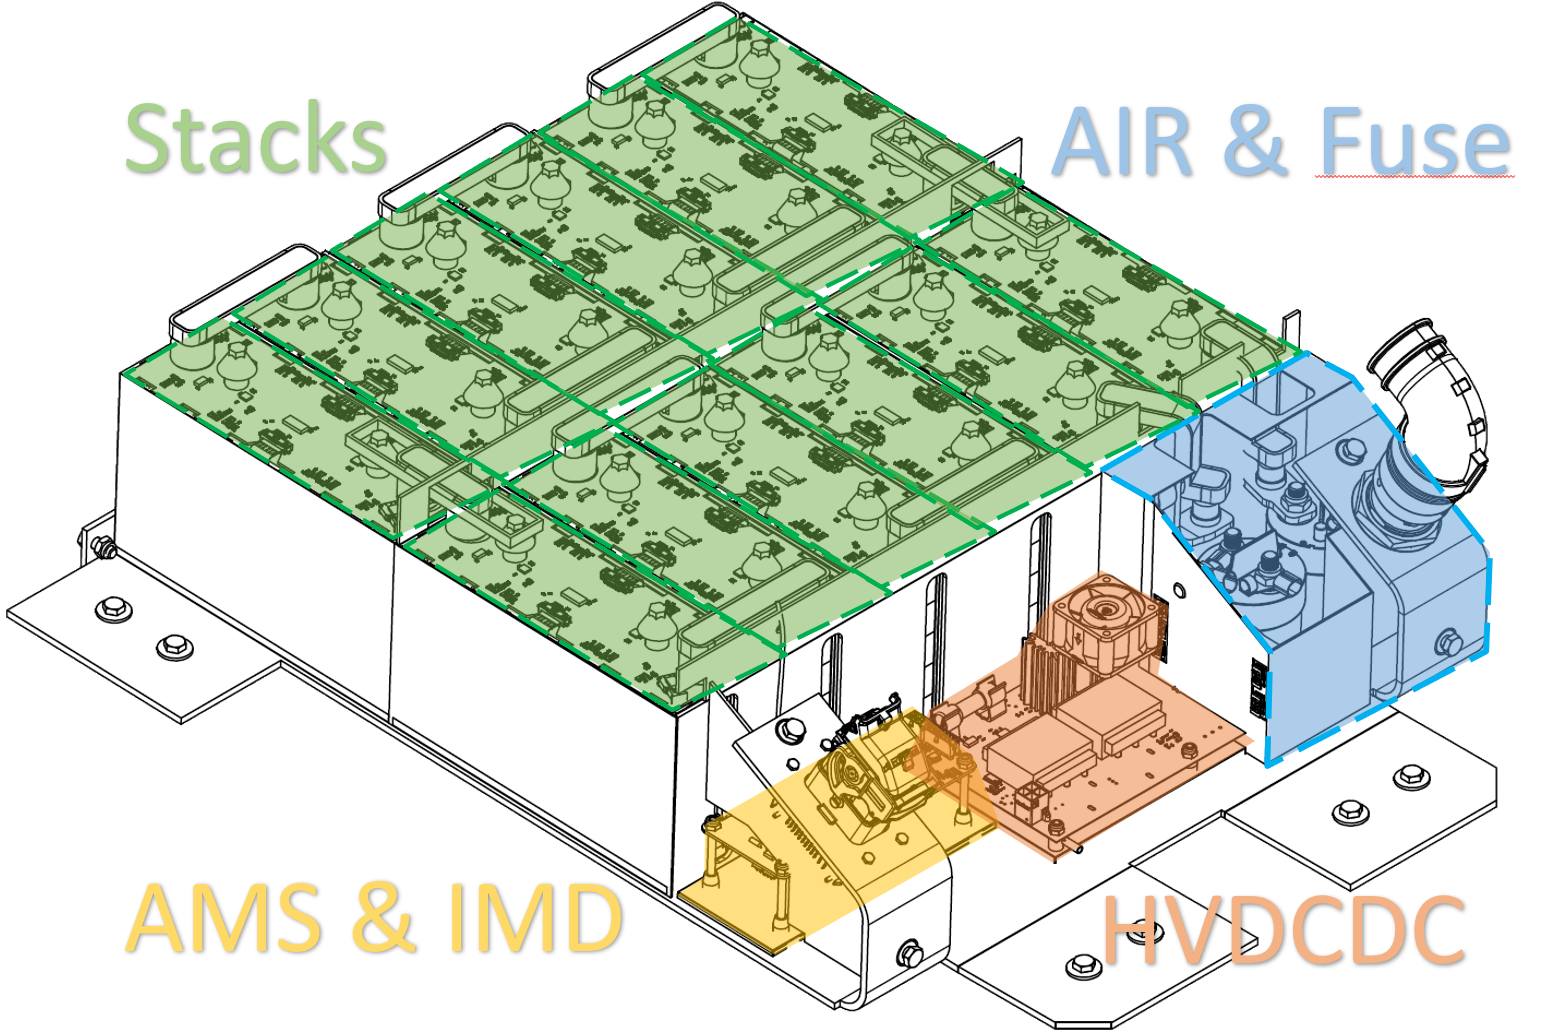
\includegraphics[width=0.7\linewidth]{bilder/HV_Akkumulator_Layout}
	\caption{}
	\label{fig:hvakkumulatorlayout}
\end{figure}


Der Akkumulatorcontainer besteht aus Aluminium. Dabei muss vom Regelwerk her der Boden mindestens \ensuremath{3,2 mm} und die wände \ensuremath{2,3 mm} Dick sein. \cite{FSRules} Gewählt wurden respektive \ensuremath{4 mm} und \ensuremath{2,5 mm}. In der ersten Version handelt es sich bei dem Container um mehrere geschweißte Biegeteile. Solch ein Konstrukt zeichnet sich jedoch durch derart starken Schweißverzug aus das bei der Folgeversion eine Kombination aus Nieten kleben, schrauben und schweißen anzuraten ist. Gerade mit dem überarbeiten Stack Konzept lässt sich eine reine Schweißkonstruktion nicht mehr umsetzten. Hierbei währen die Stackwände vernietet und verschraubt, die Bodenwanne eine Biege-Schweißteil, der Deckel ein Biegeteil und etwaige interne Anbindung für z.b die \ac{HV}-Stecker sind geklebt.

\section{Elektromotor}
Für die Auswahl des Elektromotors gibt es 5 verschiedene in der Formula Student allgemein anerkannte Lösungen. Diese werden nachfolgend erläutert.\\
\\
\textbf{Emrax}\\
Beim Emrax Motor handelt es sich um eine Axial Flux \acfirst{PMSM}. Zusammenfassend sind die Emrax Motoren sehr flach, haben aber einen großen Durchmesser. Sie zeichnen sich durch ein hohes Drehmoment und damit verhältnismäßig niedrige Drehzahlen aus, im Bereich von \ensuremath{7-8K \acfirst{RPM}}. Sie sind nur in recht großen Formaten und damit großen Leistungen erhältlich so das ein 1 oder 2 Motoren Antriebskonzept realisierbar ist. Außerdem handelt es sich hierbei um eine reine Kauflösung. \\
\\
\textbf{AMK}\\
Die AMK Motoren sind Radial Flux \ac{PMSM}. Sie sind insofern eher lang und haben kleine Durchmesser. Die Bauform gleicht insofern eher dem klassischen Elektromotor. Sie zeichnen sich durch extrem hohe Drehzahlen aus, oberhalb der \ensuremath{20k\ac{RPM}} und damit durch eine enorme Leistungsdichte. Sie sind in eher kleinen Leistungsbereichen zu bekommen so das beinahe nur ein Allradantrieb sinnvoll umsetzbar ist. Auch hierbei handelt es sich um eine reine Kauflösung. \\
\\
\textbf{Fischer}\\
Die Motoren von Fischer sind im großen und ganzen gleichzusetzen mit den AMK Motoren. Der große Unterschied ist das hier das Gehäuse selbst designt werden muss und alle Teile selber gefertigt werden müssen. Dies stellt große Herausforderungen die Fertigungstechnik da es sich dabei auch um 5-Achs gefräste Titanteile handelt.\\
\\
\textbf{Asia \& Co}\\
Eine weitere Optionen wäre es günstige Motoren eines Asiatischen Hersteller zu beschaffen, als Beispiel wäre hier die Firma Freerchhobby zu nennen, es gibt aber viele mehr. Diese Motoren zeichnen sich durch ein herausragend niedrigen Preis aus sowohl für den Motor als auch den zugehörigen Motorcontroller. Problematisch hierbei ist, das diese Motoren in der Regel nur bis Spannungsbereiche von \ensuremath{120 V} verfügbar sind. Der dabei bei \ensuremath{80 kW} resultierende Strom ist enorm. Heißt das entweder die Leistung zu reduzieren wäre oder die elektrische des Auslegung des \ac{TS} besondere Ansprüche gestellt hätte. Weiter stellt sich hier die Frage der Zuverlässigkeit. 2014 bis 2016 ist man im Racing Team einen Einzylindermotor der Firma Borossi gefahren, welcher sich durch nicht vorhandene Haltbarkeit auszeichnete und so 3 Saisons in folge torpedierte. Daher sind die anderen optionen sofern erschwinglich vorzuziehen. Sollte das Budget aber besonders eng sein, können diese Motoren durchaus eine valide Alternative darstellen.\\
\\
\textbf{Selbstbau}\\
Der Selbstbau ist die nächste Entwicklungsstufe nach dem Fischer Motor. Nun gilt es nicht nur den Motor selber zu Fertigen sondern auch die gesamte Vorauslegung zu machen. Es gibt nur wenige Teams die einen Selbstbau wagen, und noch weniger setzen es erfolgreich um.\\
\\
\textbf{Entscheidungsfindung}\\
Im Rahmen dieser Projektarbeit soll das Konzept für den ersten E-antrieb unseres Formula Student Teams entstehen. Damit kommen bereits viele Herausforderungen, so das wenn möglich der Aufwand und die Komplexität zu verringern ist. Damit wurde sich für den Emrax Motor entschieden, da ein Selbstbau als auch nein Allradantrieb nicht zur Option standen

\section{Wechselrichter}
Der Wechselrichter wird benötigt um den Motor sauber anzusteuern. Ziel ist es aus Gleichstrom aus dem Akku einen Frequenz und Amplituden regelbaren Strom zu erzeugen mit dem der Motor kontrolliert werden kann. Hier gibt es auch wieder diverse Hersteller die im folgenden verglichen werden sollen

!!!Tabelle!!! mit daten

\section{Kabelbaum} %(zusammen mit Nico Bieberich)
Der Kabelbaum lässt sich bei einem Elektrofahrzeug in mehrere Funktionsgruppen unterteilen. Einmal haben wir den Datenbus zur Kommunikation der Steuergeräte im Fahrzeug. In unserem Fall ist das ein \acfirst{CAN}-Bus. Dann den sogenannten \ac{SDC} zur Absicherung der Systeme bzw. einleiten eines sicheren Zustandes in dem Fall das ein Fehler auftritt. Weiter gibt es die Gruppe der \ac{HV}-Kabel dies umfasst Leistungsführende Leiter für Akku, Umrichter und Motor als auch \ac{HV}-Signalleiter für z.b. die \ac{TSMP}. Dann haben wir noch die \ac{LV}-Versorgung für alle Systeme im Fahrzeug. Dann gibt es den Sensorbaum, dieser umfasst die Versorgungs- als auch Daten/-Leitungen für jegliche Sensorik im Fahrzeug. Abschließend gibt es noch alles andere was sich nicht hierunter kategorisieren lässt. Dies umfasst z.b einzelne analoge oder digitale Datenleitungen wie z.b die Ethernet Leitung für den \ac{FSG} Logger oder die Abzweigleitung des Bremsdruckes für das \ac{BSPD}. Auf die einzelnen Gruppen wird im folgenden detailliert eingegangen.\\
\\
Wichtige generelle Überlegungen beim Kabelbaum sind jegliche Maßnahmen die den Kabelstrang \acfirst{DAU} sicher machen. Sprich verpolsichere Steckverbinder. Belegung der Stecker so, dass ohne Verpolschutz kein Kapitalschaden eintritt. Auswahl des richtigen Steckers für die "heiße" Seite, heißt der Steckverbinder der uneingesteckt unter Spannung steht sollte ein Berührungsschutz aufweisen. Logische Farbcodierung sowohl der Kabel, als wenn möglich auch der Steckverbinder, sodass beim Zusammenbau keine Fehler gemacht werden und dies einheitliche über Jahre durchgängige geführt und damit auch Dokumentiert.\\
\\
Die Dokumentation hierfür finden sie in den folgenden Tabellen \ref{tab:steckertypen}, \ref{tab:Kabel&SteckerFarbtabelle}

\begin{table}
	\label{tab:steckertypen}
	\caption{Steckertypen Tabelle}
\begin{tabular}{|c|c|c|c|c|c|}
	
	\hline
	\multicolumn{6}{|c|}{Steckertypen} \\
	\hline
	Name & W2W/W2B & Montage & Sealed & Einsatzbereich & Pinanzahlen \\
	\hline
	Molex Micro Fit & both & Wire & no & HV/LV & 2-20 \\
	\hline
	Molex CMC/CMX & W2B & Panel & Yes & LV  & 28-154 \\
	\hline
	TE HD10/20/30 & both & both & Yes & HV & 3-47 \\
	\hline
	Molex Mizu P 25 & W2W & Wire & Yes & LV & 2-4 \\
	\hline
	Binder Sub M9 & both & both & Yes & LV & 2-8 \\
	\hline
	Binder M12 Power & both & both & Yes & HV & 2-8 \\
	\hline
	Würth WRBHD2.54 & W2B & Wire & No & LV & 10 \\
	\hline
\end{tabular}
\end{table}

\begin{table}
	\centering
	\label{tab:Kabel&SteckerFarbtabelle}
	\caption{Kabel \& Stecker Farbtabelle}
\begin{tabular}{ll}
	
\begin{tabularx}{8cm}{|c|c|}
	\hline
	\multicolumn{2}{|c|}{\textbf{\large {Farbtabelle}}} \\
	\hline
	Farbe & Signal \\
	\hline
	\multicolumn{2}{|c|}{\textbf {Kabel}} \\
	\hline
	White & 24V \\
	\hline
	\cellcolor{brown!30} Brown & GND \\
	\hline
	\multicolumn{1}{|@{}X@{}|}{\tikzmark[a]{Brown Green}} & CANH/Signal\\
	\hline
	\cellcolor{yellow!30} Yellow & CANL/5V \\
	\hline
		\hline
	\multicolumn{2}{|c|}{\textbf {Leiter}} \\
	\hline
	White & 24V \\
	\hline
	\multicolumn{1}{|@{}X@{}|}{\tikzmark[b]{White Yellow}} & 5V\\
	\hline
	\multicolumn{1}{|@{}X@{}|}{\tikzmark[c]{White Pink}} & 12V\\
	\hline
	\multicolumn{1}{|@{}X@{}|}{\tikzmark[d]{White Red}} & 3V\\
	\hline
	\cellcolor{brown!30} Brown & GND \\
	\hline	
	\cellcolor{green!30} Green & CANH \\
	\hline
	\cellcolor{yellow!30} Yellow & CANL \\
	\hline
	\cellcolor{blue!30} Blue & SDC \\
	\hline
	\multicolumn{1}{|@{}X@{}|}{\tikzmark[e]{Blue Red}} & SDC\textsubscript{end} \\
	\hline
	\multicolumn{1}{|@{}X@{}|}{\tikzmark[f]{Blue White}} & SDC\textsubscript{indicator} \\
	\hline
	\cellcolor{violet!30} Voilet & Signal \\
	\hline
		\hline
	\multicolumn{2}{|c|}{\textbf {HV-Leiter}} \\
	\hline
	\cellcolor{red!30} Red & TSMP+/HV+ \\
	\hline
	\cellcolor{black!30} Black & TSMP-/HV- \\
	\hline
	\cellcolor{blue!30} Blue & SDC \\
	\hline
		\hline
	\multicolumn{2}{|c|}{\textbf {Mehrader}} \\
	\hline
	\cellcolor{yellow!30} Yellow & LAN \\
	\hline
\end{tabularx}

\begin{tikzpicture}[remember picture,overlay]
	\path[fill=brown,opacity=0.3](a.north west)--(a.south west) -- (a.south east) -- cycle;
	\path[fill=green,opacity=0.3](a.north east)--(a.south east) -- (a.north west) -- cycle;
	
	\path[fill=white,opacity=0.3](b.north west)--(b.south west) -- (b.south east) -- cycle;
	\path[fill=yellow,opacity=0.3](b.north east)--(b.south east) -- (b.north west) -- cycle;
	
	\path[fill=white,opacity=0.3](c.north west)--(c.south west) -- (c.south east) -- cycle;
	\path[fill=pink,opacity=0.3](c.north east)--(c.south east) -- (c.north west) -- cycle;
	
	\path[fill=white,opacity=0.3](d.north west)--(d.south west) -- (d.south east) -- cycle;
	\path[fill=red,opacity=0.3](d.north east)--(d.south east) -- (d.north west) -- cycle;
	
	\path[fill=blue,opacity=0.3](e.north west)--(e.south west) -- (e.south east) -- cycle;
	\path[fill=red,opacity=0.3](e.north east)--(e.south east) -- (e.north west) -- cycle;
	
	\path[fill=blue,opacity=0.3](f.north west)--(f.south west) -- (f.south east) -- cycle;
	\path[fill=white,opacity=0.3](f.north east)--(f.south east) -- (f.north west) -- cycle;
\end{tikzpicture}


\begin{tabularx}{6cm}{|c|c|}
	\hline
	\multicolumn{2}{|c|}{\textbf{Mizu P25}} \\
	\hline
	\multicolumn{2}{|c|}{\cellcolor{black!30} CAN Schwarz 4Pin} \\
	\hline
	\cellcolor{brown!30} GND & 1 \\
	\hline
	\cellcolor{green!30} CANH & 2 \\
	\hline
	\cellcolor{white!30} 24V & 3 \\
	\hline
	\cellcolor{yellow!30} CANL & 4 \\
	\hline
		\hline
	\multicolumn{2}{|c|}{\cellcolor{white!30} Sensor Weiß 4Pin} \\
	\hline
	\cellcolor{brown!30} GND & 1 \\
	\hline
	\cellcolor{yellow!30} 5V & 2 \\
	\hline
	\cellcolor{white!30} 24V & 3 \\
	\hline
	\cellcolor{green!30} Signal & 4 \\
	\hline
		\hline
	\multicolumn{2}{|c|}{\cellcolor{black!30} SDC Schwarz 3Pin} \\
	\hline
	\cellcolor{blue!30} SD\textsubscript{in} & 1 \\
	\hline
	\cellcolor{blue!30} SD\textsubscript{out} & 2 \\
	\hline
	\multicolumn{1}{|@{}X@{}|}{\tikzmark[g]{SDC\textsubscript{indicator}}} & 3 \\
	\hline
		\hline
	\multicolumn{2}{|c|}{\cellcolor{white!30} Servos Weiß 3Pin} \\
	\hline
	\cellcolor{yellow!30} Signal & 1 \\
	\hline
	\cellcolor{brown!30} GND & 2 \\
	\hline
	\cellcolor{red!30} 8.3V & 3 \\
	\hline
		\hline
	\multicolumn{2}{|c|}{\cellcolor{white!30} Brakelight Weiß 3Pin} \\
	\hline
	\cellcolor{violet!30} Signal & 1 \\
	\hline
	\cellcolor{brown!30} GND & 2 \\
	\hline
	\cellcolor{red!30} 24V & 3 \\
	\hline
	\multicolumn{2}{|c|}{\textbf{Binder SubM9}} \\
	\hline
	\multicolumn{2}{|c|}{\cellcolor{black!30} CAN 4Pin} \\
	\hline
	\cellcolor{brown!30} \centering{GND} & 1 \\
	\hline
	\cellcolor{green!30} \centering{CANH} & 2 \\
	\hline
	\cellcolor{white!30} \centering{24V} & 3 \\
	\hline
	\cellcolor{yellow!30} \centering{CANL} & 4 \\
	\hline
\end{tabularx}

\begin{tikzpicture}[remember picture,overlay]
 	\path[fill=blue,opacity=0.3](g.north west)--(g.south west) -- (g.south east) -- cycle;
	\path[fill=white,opacity=0.3](g.north east)--(g.south east) -- (g.north west) -- cycle;
\end{tikzpicture}

\end{tabular}

\end{table}
\FloatBarrier
\subsection{\ac{CAN}-Bus}
Beim \ac{CAN}-Bus handelt es sich um ein Multi-Master Bus mit zwei normalerweise verdrillten symmetrischen Datenleitungen. Wichtig zu beachten ist das der \ac{CAN}-Bus immer als Linientopologie aufgebaut werden sollte und dabei die Anzahl an Stichleitungen möglichst klein zu halten ist. Weiterhin muss an den enden der Linie ein \ensuremath{120 \Omega} Widerstand eingesetzt werden. Für Stichleitungen empfiehlt sich bei Problemen in der Buskommunikation ein \ensuremath{4,7 k\Omega} Widerstand zur Terminierung der Datenleitungen einzusetzen.

\subsection{\ac{LVS} Versorgung}

Die \ac{LVS} Versorgung läuft in einer Sterntopologie von der Fusebox aus. Hier befinden sich die mittels Mikrocontroller überwachten Sicherungen für alle elektrischen Verbraucher. Ausnahmen hiervon sind die Versorgung des \ac{SDC} welcher am \acfirst{LVMS} starten muss als auch die Versorgung des \ac{BSPD} welches direkt vom \ac{LVMS} versorgt werden muss. Die Versorgung der Steuergeräte welche per \ac{CAN}-Bus mit der Fusebox verbunden sind läuft zusammen in einem 4 Ader Kabel mit dem \ac{CAN}-Bus und entspricht daher eher einer Linientopologie. Die Masseleitung laufen an insgesamt 3 verschiedenen Sternpunkten auf das Chassis zusammen. Einer befindet sich am abnehmbaren Heck des Fahrzeuges, einer rechts hinter der Firewall im Fahrzeug und einer im Vorderbau des Fahrzeuges.

\subsection{Sensor Kabelbaum}

Der Sensorkabelbaum besteht aus beinahe ausschließlich 4 Ader Kabeln welche \ensuremath{24 V}, \ensuremath{5 V}, GND und ein Signal führen. Diese Kabel laufen sternförmig von jedem der Sensorhubs zu den entsprechenden Sensoren.

\subsection{\ac{SDC}}
\begin{figure}[h]
	\centering
	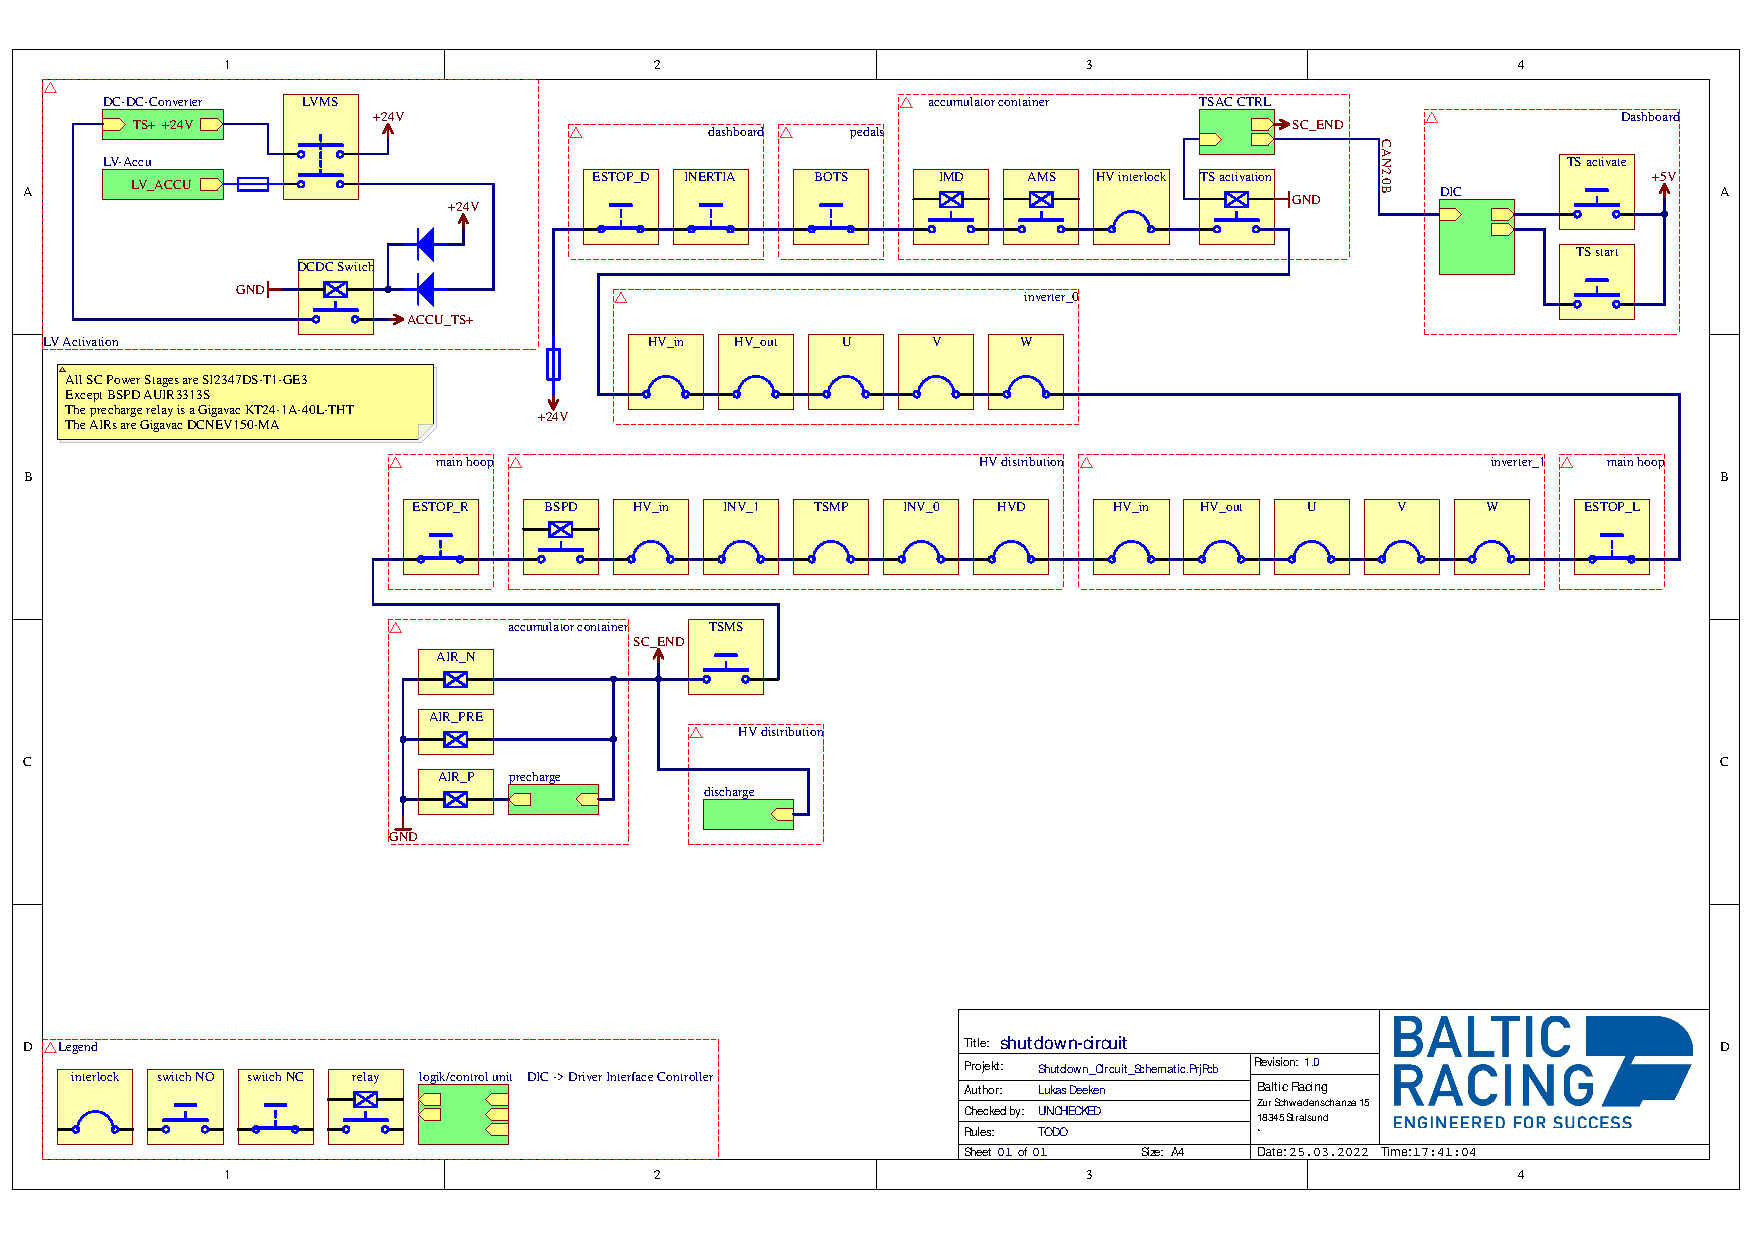
\includegraphics[width=1\linewidth]{bilder/Shutdowncircuit}
	\caption{\ac{SDC} Schaltplan}
	\label{fig:shutdowncircuit}
\end{figure}

In der obenstehenden Graphik ist der sogenannte \ac{SDC} abgebildet. Oben Links befindet sich die Versorgung bzw. der Anfang des \ac{SDC} bestehend aus dem Kickstarter für den \ac{HV}-DCDC und der Hauptschaltung für den \ac{LVMS}. Oben rechts befindet sich die \ac{TS}-aktivierungs-Logik. Im Dashboard des Fahrzeuges befinden sich 2 Knöpfe, einer um das \ac{TS} einzuschalten und einer um die Motoren freizuschalten und damit das Losfahren zu ermöglichen. Die Kommunikation erfolgt hier über den \ac{CAN}-Bus direkt zum \ac{AMS}-Master. Auf dem Rest des Schaltplanes ist von oben nach unten der gesamte \ac{SDC} mit all seinen Elementen abgebildet. Am ende des \ac{SDC} befinden sich die \ac{AIR}`s welche direkt vom \ac{SDC} betrieben werden müssen. Weiterhin wird dort das \ac{SDC}\textsubscript{END}-Signal abgezweigt welches den Ausgangsstatus des \ac{SDC} abzweigt und z.b dem Discharge bereitstellt.\\
\\
Wichtig beim \ac{SDC} zu beachten ist das an möglichst vielen Stellen Stichleitungen eingebracht werden um den \ac{SDC} überwachen zu können. Dies hilft enorm bei der Fehlereingrenzung. Weiter sollte der Querschnitt der Kabel nicht zu dünn gewählt sein. Der Strom im \ac{SDC} liegt bei ca. \ensuremath{0,24 A}, da hierüber die \ac{AIR}`s direkt geschaltet werden müssen und hat am ende eine beträchtliche Länge im Fahrzeug und damit einen nicht zu vernachlässigen Widerstand. 
\FloatBarrier
\subsection{Kabeldimensionierung}
%Quelle
Bei Der Kabeldimensionierung wurden 2 unterschiedliche Ansätze angewandt. Einmal die Dimensionierung nach DIN VDE 0298-4 \cite{DINVDE02984} und einmal anhand der Tabelle \ref{fig:wire-thickness}. Zweiteres empfiehlt sich standardmäßig für so gut wie alle Anwendungen. Ersterer ist hierbei nur für die Stromführenden \ac{HV}-Leiter sinnvoll anzuwenden. Die Querschnittberechnung ließe sich mit einem physikalischen Modell noch weiter treiben, auf dies wurde jedoch aufgrund des Zeitmangels verzichtet.
Folgend ist einmal die bisher verwendete Tabelle \ref{fig:wire-thickness} aufgeführt.
Bei der Tabelle ist zu beachten das die Ströme für Chassis Wiring verwendet werden. Unter Power Transmission versteht man hier Leiter die mit geringen Verlusten z.b in einer industriellen Umgebung Ströme über lange Wege z.b. von Haus zu Haus leiten sollen.
\begin{figure}[h]
	\centering
	\includegraphics[width=0.7\linewidth]{"bilder/Wire thickness"}
	\caption{Leiterquerschnitts-Tabelle \cite{Technology2022}}
	\label{fig:wire-thickness}
\end{figure}

Nun soll im Anschluss einmal die Berechnung der Querschnitte nach DIN VDE 0298-4 (Anhang) dargestellt werden.\\
Nach 9.4 können wir für ungleichmäßige Ströme den Quadratischen Mittelwert zur Leiterquerschnittbestimmung ansetzen. Den Quadratischen Mittelwert des Stromes der Elektromotoren erhalten wir indem wir das mittlere Drehmoment am Elektromotor bestimmen, hierfür müssen wir auf die Daten aus der \ac{LTS} zurückgreife, in Zukunft empfiehlt es sich die Berechnung einmal mit den Daten aus dem tatsächlichen Fahrzyklus nachzurechnen. Das Drehmoment was wir hier erhalten liegt bei \ensuremath{68,2 Nm} pro Motor. Im Handbuch des Emrax 208 (Anhang) befindet sich ein Parameter der uns den \acfirst{RMS}-Strom in A pro NM Drehmoment an der Ausgangswelle angibt. Dieser liegt bei \ensuremath{0,8 Nm/A\textsubscript{RMS}}. \\
Damit lässt sich ermitteln das der Quadratische Mittelwert des Stromes bei ca. \ensuremath{85,3 A} liegt\\
Nun lässt sich mit Hilfe von Tabelle 9.2 der Strom für den Verlegungstyp E (Verlegung wie Motorleiter) für verschiedene Kabelquerschnitte ermitteln. Wir ermitteln für \ensuremath{16 mm^2} einen Strom von \ensuremath{80 A} für 3 belastete Leiter und für \ensuremath{25 mm^2} respektive einen Strom von \ensuremath{101 A}. Zur Sicherheit wurde hier an der Stelle auf \ensuremath{25mm^2} zurückgegriffen, allerdings sollten in Zukunft durchaus mal Versuche mit \ensuremath{16 mm^2} für die Motorleiter unternommen werden da dies zu einer durchaus signifikanten Gewichtsersparnis führen kann.\\
\\
Für den \ac{DC}-Bus wurde das gleiche vorgehen angewandt. Hier bekommen wir den Strom direkt aus der \ac{LTS} mit \ensuremath{53A}. Das ergibt nach Typ E mit 2 belasteten Leitern \ensuremath{10 mm^2} Querschnitt. Jedoch konnten wir keine Steckverbinder finden welche \ensuremath{10 mm^2} Kabel akzeptiert und ein entsprechendes Rating hat weshalb wir hier auf \ensuremath{16 mm^2} und damit einen max. Strom von \ensuremath{80 A} gegangen sind. Auch hier gilt wieder das noch Möglichkeiten der Gewichtsersparnis bestehen.\\

\FloatBarrier
\subsection{Hochvolt Kabelbaum}

\begin{figure}[h]
	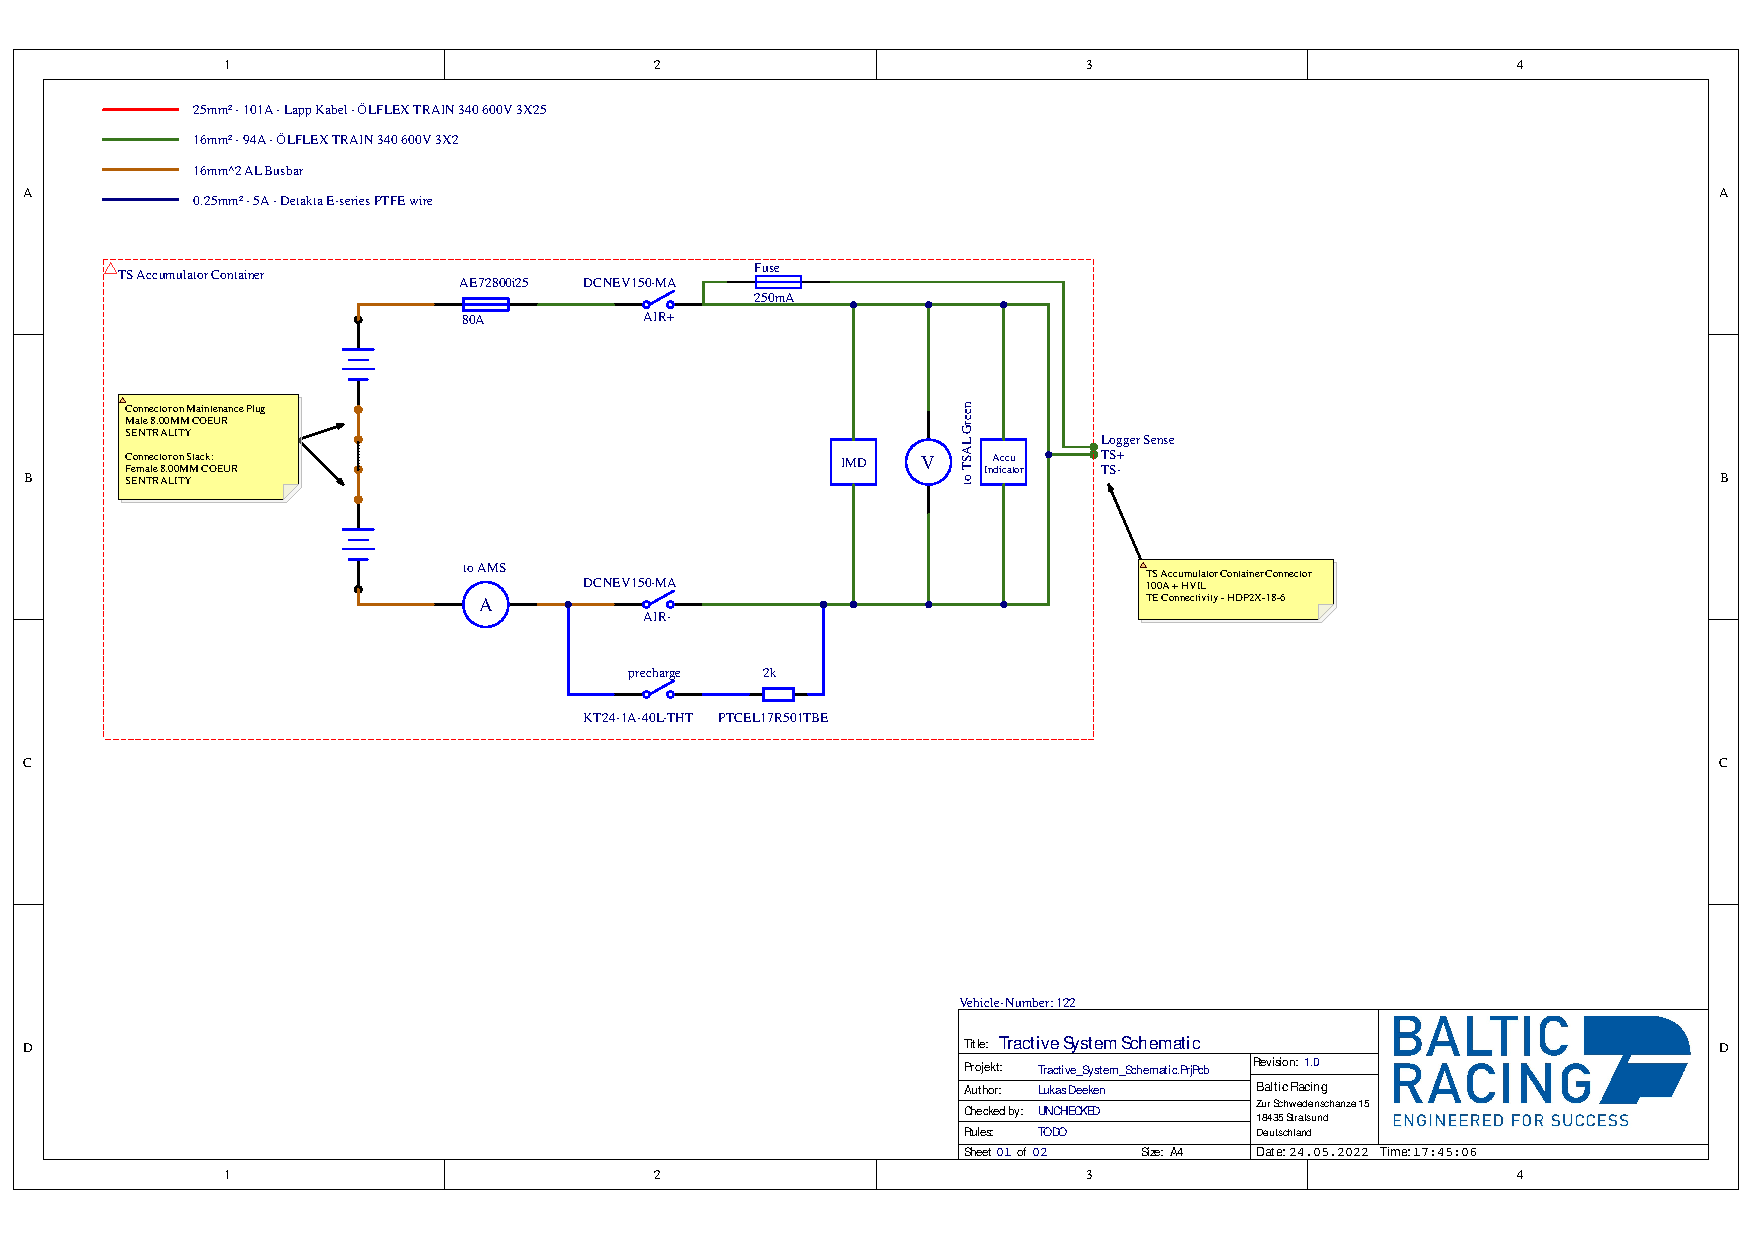
\includegraphics[page=1,width=1\linewidth]{bilder/Tractive_System_Schematic_V4.pdf}
	\caption[\ac{TS} Schaltplan Seite 1]{}
	\label{fig:tractivesystemschematic1}
	
	\includegraphics[page=2,width=1\linewidth,]{bilder/Tractive_System_Schematic_V4.pdf}
	\caption[\ac{TS} Schaltplan Seite 2]{}
	\label{fig:tractivesystemschematic2}
	\end{figure}

Der HV Kabelbaum besteht aus 3 Kabelsträngen, einer befindet sich innerhalb des Akkus, einer innerhalb der \ac{HV}-Distribution und einer verbindet diese beiden Geräte sowie die Motoren und die Umrichter miteinander.\\
\\
Wichtig zu beachten ist das alle \ac{HV}-Kabel Orange und entsprechend isoliert sein müssen. Außerdem dürfen \ac{HV}- und \ac{LV}/-Kabel nicht zusammen verlegt werden bzw. sollte es der Fall sein müssen die \ac{LV}-Kabel auch nach \ac{HV} Spezifikation isoliert sein.\\
Es gilt besondere Achtsamkeit bei den Leiterquerschnitten sowie den Mindestbiegeradien an den Tag zu legen. Bei den Steckern ist besonders das Spannungsrating Problematisch, da hier gerne nur das \acfirst{AC}- oder \ac{DC}/-Rating gegeben wird und hier dann entsprechend umzurechnen ist. Hierbei wird das \ac{AC}-Rating mal 1,41 gerechnet um das korrespondierende \ac{DC}-Rating zu erhalten. \\
\\
Bei den \ac{HV}-Leitern ist die Möglichkeit von Aluminium Leitern interessant. Hier wurde damals von der Firma Coroflex die Zusage gemacht das sollte ein Auftrag für ein derartiges Kabel reinkommen, würde man für das Team eine entsprechende Menge kostenlos mit fertigen. Evtl. ließe sich hier in Zusammenarbeit mit anderen Teams eine nennenswerte Menge abnehmen so das sich die Produktion für ein Unternehmen lohnt. Hierbei allerdings beachten das die bisherige Dimensionierung nur für Kupferkabel gilt und dementsprechend im besten Fall noch einmal mit dem Unternehmen zusammen durchgeführt werden sollte.\\
\\
Ansonsten gilt zu beachten das man gerade diese Mehradrigen Kabel, sprich Kabel mit 3 mal \ensuremath{25 mm^2}, wie sie dieses Jahr verwendet werden nicht serienmäßig in orangener Ausführung bekommt, was bedeutet, dass man das Kabel auf jeden Fall einmal in orangenen Schrumpfschlauch einschrumpfen muss. In diesem Zuge wurde auch die Schirmung um die Kabel selbst eingebracht da dies im Gegensatz zur kommerziellen Lösung eine Gewichtsersparnis von ca. \ensuremath{1 kg} auf das gesamte Fahrzeug brachte. Außerdem sollten jegliche Stellen wo die Isolierung der \ac{HV}-Kabel verletz wird z.b an Kabelschuhen etc. immer ein Schrumpfschlauch mit Innenkleber angebracht werden. Es empfehlen sich besonders Schläuche mit einem Schrumpfungsverhältnis 3:1. Hierbei gilt zu beachten das es diese Schläuche \ac{idR} auch nicht in Orange gibt weshalb in dem Fall immer ein Klebeschrumpfschlauch als auch ein orangener angebracht werden sollte. Für die mehradrigen Kabel wurde sich entschieden da diese insgesamt eine Gewichtsersparnis bringen und am Ende für ein deutlich saubereres und ordentlicheres Gesamtbild sorgen. Bei der Montage der \ac{HV}-Leiter ist zu beachten das alle Verbindungen bei der Montage wie z.b. die Verschraubung der Kabelschuhe an die \ac{TSMP} fotografiert werden bevor sie in Schrumpfschlauch etc. eingepackt werden. Dies ist für die technische Abnahme notwendig, damit der Prüfer die saubere Montage der Verbindung überprüfen kann, ohne das etwaiger Schrumpfschlauch wieder entfernt werden muss. Weiterhin hat Isoband im Bereich \ac{HV} absolut keine sichere Wirkung und wird auch von der \ac{FSG} nicht als adäquater Isolator angesehen. Für alle Verbindungen etc. gilt stets diese nach Datenblatt zu machen. Heißt wenn beim \ac{TSMP}-Steckverbinder eine schraube und eine Mutter dabei sind dann werden diese verwendet und nicht Mechanismen zur Schraubensicherung erdacht. Weiterhin gilt zu beachten das jeder einzelne stromführende Leiter einzeln abgesichert sein muss. Dies erschwert z.b das parallel schalten von mehreren Pins in einem Steckverbinder zum leiten des Stromes da dann am Steckverbinder für jeden parallelen Kontakt entsprechende Sicherungen vorgesehen sein müssen. Dem aufmerksamen Leser fällt an dieser Stelle auf das bei dem Elektromotor in allen drei Leitern keine separaten Sicherungen vorgesehen sind. Dies lässt sich darauf zurückführen das der Umrichter zugekauft ist und laut Datenblatt über einen entsprechenden Überstromschutz verfügt. Im Selbstbau Fall müssten hier 3 Sicherungen wie aus dem Akku bekannt verbaut werden. 
 
 \FloatBarrier
\subsection{Sicherungsauslegung}
Die Sicherung muss stets der schwächste Teil eines Stromkreises sein. In diesem Sinne muss also bei der Auslegung der Stecker darauf geachtet werden das deren Rating höher ist als das der Sicherung oder wir müssen im Umkehrschluss schauen dass, das Rating der Sicherung niedriger ist als das der anderen Komponenten. Für \ac{DC}-Sicherungen mit einer derart hohen Betriebsspannung und einem derart hohen Kurzschlussstrom reichen Flachstecksicherung wie sie im \ac{LV}-Bereich zu finden sind nicht mehr aus. Hier müssen z.b sandgefüllte Sicherungen verwendet werden. Sinn dahinter ist es den Lichtbogen der sich beim durchbrennen der Sicherung bildet zu löschen. Dies ist bei einer typischen \ac{LV}-Sicherung nicht gegeben. \\
Zum Thema Kurschlussrom, dieser errechnet sich aus dem Innenwiederstand des gesamten Akkus und der anliegenden Spannung. Wir Rechnen hier immer im schlimmsten Fall sprich alle Zellen sind was den Innenwiederstand angeht eher im niedrigeren Bereich und der Akku ist voll geladen.\\
\\
Die Formel für den Innenwiederstand des Akkus ergibt sich aus der Parallel und Reihenschaltung der identischen Innenwiederstände der Akkuzelle.

\begin{equation}
	\glsc{symb:R_Akku} = \dfrac{\glsc{symb:R_cell}} {\glsc{symb:N_Parallel}} * \glsc{symb:N_Seriell}
\end{equation}

Die Formel für den Spannung.

\begin{equation}	
	\glsc{symb:U_Akku} = \glsc{symb:N_Seriell} * \glsc{symb:U_cell}
\end{equation}

Die Formel für den Kurzschlussstrom.

\begin{equation}
	\glsc{symb:I_Akku} = \dfrac{\glsc{symb:U_Akku}}{\glsc{symb:R_Akku}}
\end{equation}

\begin{table}[h]
	\centering
	\begin{tabular}{|c|c|c|}
		\hline
		\multicolumn{3}{|c|}{Eingangswerte} \\
		\hline
		\glsc{symb:R_cell} & 8 & \ensuremath{m\Omega} \\
		\hline		
		\glsc{symb:U_cell} & 4,25 & \ensuremath{V} \\
		\hline
		\glsc{symb:N_Parallel} & 5 & \ensuremath{-} \\
		\hline
		\glsc{symb:N_Seriell} & 132 & \ensuremath{-} \\
		\hline		
		\multicolumn{3}{|c|}{Ergebnisse} \\
		\hline
		\glsc{symb:R_Akku} & 211,2 & \ensuremath{m\Omega} \\
		\hline
		\glsc{symb:U_Akku} & 561 & \ensuremath{V} \\
		\hline		
		\glsc{symb:I_Akku} & 2656 & \ensuremath{A} \\
		\hline
	\end{tabular}
\end{table}

Der Kurzschlussstrom sollte mit dem rated breaking current verglichen werden. Ist der Kurzschlussstrom niedriger ist die Sicherung geeignet. Dann haben wir bei der Sicherung das Spannungsrating welches eingehalten werden muss. Auf Basis dieser Daten kann eine Sicherung bzw. eine Baureihe herausgesucht werden. In unserem Fall ergaben die Recherchen die AE7 EV Fuse von Adler Elektrik. Die Querschnittberechnung hat ein Kabel von \ensuremath{16 mm^2} und daher \ensuremath{80 A} ergeben. Diese \ensuremath{80 A} legen wir auch bei der Sicherung zu Grunde. Dies ergibt die AE72800i25 \cite{AE7Specification}. Daraufhin lässt sich im Datenblatt am Zeit-Strom Schaubild \ref{fig:zeitstromtsfuse} ablesen wie lange die Sicherung bei Unterschiedlichen Strömen braucht um auszulösen. Es ergibt sich eine zeit von ca. \ensuremath{400 s} bei einem Strom von \ensuremath{150 A} und eine Zeit von ca. \ensuremath{0,5 ms} bei Kurzschlussstrom.

\begin{figure}[h]
	\centering
	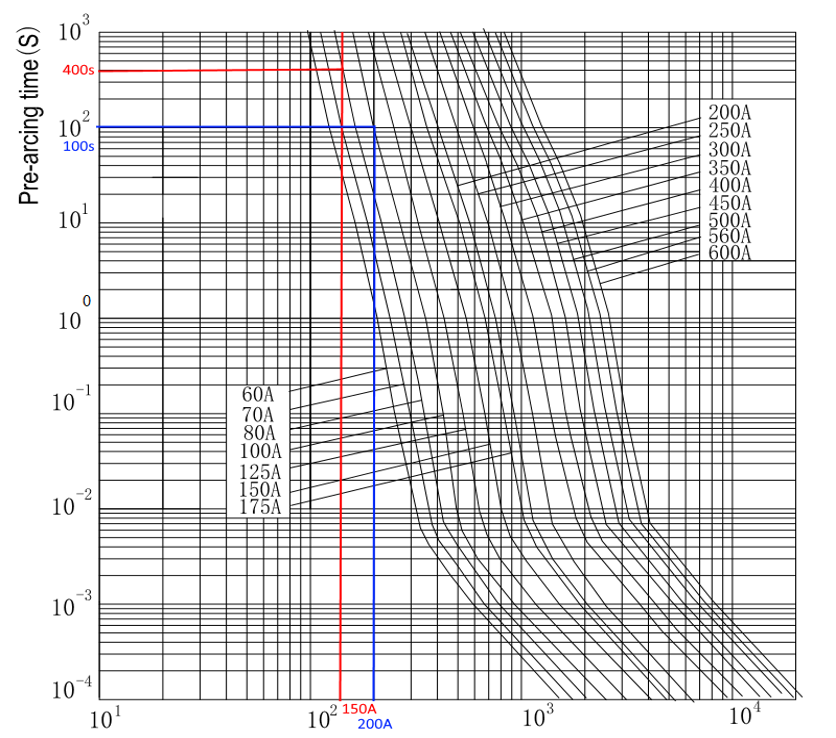
\includegraphics[width=0.7\linewidth]{bilder/Zeit_Strom_TSFUSE}
	\caption{}
	\label{fig:zeitstromtsfuse}
\end{figure}

\FloatBarrier
\subsection{Steckverbinder Auswahl}
Parameter für die Steckverbinder Auswahl sind analog zur Kabelauswahl, die Betriebsspannung als auch der Betriebsstrom. Die Auswahl der Steckverbinder erfolgt im Zuge des Systemdesigns wo die Schnittstellen und die Anforderungen an diese festgelegt wurden. Der gewählte Steckverbinder sollte über ausreichend Plätze in der richtigen Stärke verfügen um den Anforderungen gerecht zu werden. Hierbei ist interessant welche Pins man für die Steckplätze bekommen kann. Oft ist es so möglich durch unterschiedlich große Steckplätze die gleichen Kabelquerschnitte zu bekommen. Da es selten Steckverbinder gibt die genau zu dem vorliegenden System passen kann dies sehr nützlich sein um das einsetzten eines deutlich größeren und damit schwereren als auch teureren Steckverbinders zu verhindern. Auch bei den Pins gilt es stets die Stromratings zu beachten. Bei gerade solchen Kabel zu Kabel Verbindern die dazu dienen Kabel in ein Gehäuse zu führen ist es sinnvoll ein paar Steckplätze im Design frei zu lassen um es zu ermöglichen im Nachhinein einfach weitere Kabel hinzuzufügen, sollte dies später einmal notwendig werden. Auch führt dies dazu dass bei Änderung am Systemdesign die Interfaces der Geräte potentiell gleich bleiben können, was den Test und Aufbauprozess des Fahrzeuges vereinfacht. 
Bei der Auswahl der Steckverbinder ist immer drauf zu achten das entsprechende Crimp- als auch Auspinn- bzw. Einpinn/-Werkzeuge mit beschafft werden damit die Montage der Verbinder anschließend auch reibungsfrei klappt. Weiter ist auf zusätzliches Kabelzubehör wie Endkappen, Blindstecker, Staubschutzkappen usw. zu achten bzw. mit zu beschaffen. Außerdem ist es üblich die Gehäuse der Steckverbinder und die Pins separat zu bestellen sodass auch hierauf geachtet werden muss. Gerade bei der Beschaffung der Pins empfiehlt es sich mindestens um den Faktor 1,5 mehr zu bestellen als benötigt da hier öfter Ausschuss produziert wird. Auch die Steckverbinder können beim Ein- bzw. Aus/-pinnen kaputt gehen so das man hiervon Ersatz vorhalten sollte.\\
Eine Besonderheit bei den \ac{HV}-Steckern stellt die Interlockleitung dar. Ziel dieser Leitung ist es das \ac{HV}-System abzuschalten sobald ein Steckverbinder gezogen wird um einen elektrischen Schlag durch berühren der Kontakte im Steckverbinder zu verhindern. Hierbei handelt es sich meist um ein oder zwei weitere Steckkontakte im \ac{HV}-Stecker wo Kabel mit deutlich geringerem Querschnitt angeschlossen werden können. Wichtig hierbei ist das diese Interlockleitung aufgehen muss bevor eine vollständige Trennung des Steckverbinder erfolgt. 

\FloatBarrier
\subsection{\acfirst{HVD}}
Der \ac{HVD} befindet sich mittig am Heck des Fahrzeuges. Sinn dieses Steckverbinders ist es eine mechanische und damit elektrische Öffnung des \ac{HV}-Systems zwischen Akku und Umrichter zu ermöglichen. Dies kann notwendig werden wenn z.b. die \ac{AIR}`s den Dienst verweigern und damit eine Möglichkeit der Trennung der Motoren vom Betriebsstrom anderweitig nicht mehr möglich machen. Bei diesem Steckverbinder kann es sich entweder um dafür vorgesehene Service Trennschalter aus einem regulären Elektrofahrzeug handeln oder um modifizierte Steckverbinder welche auch für den Akku verwendet werden. Die modifizierten sind dabei in der Regel kleiner, leichter und günstiger.

\FloatBarrier
\subsection{\ac{AIR}}
Datenblatt werte, worauf muss ich achten
Break Open Current

Zeichnung zu diesem relai typ

Die \ac{AIR}`s haben es zum ziel das \ac{HV}-Netz des Akku galvanisch vom restlichen Fahrzeug zu trennen indem mit einem Relais \ac{HV}+ und mit dem anderen Relais \ac{HV}- geöffnet wird. Bei diesen Relais handelt es sich in der Regel um, \acfirst{SPST} \acfirst{NO} Relais mit \acfirst{AUX} Kontakten. Heißt wir haben einen Steuerkreis und einen Lastkreis. Im stromlosen Zustand ist der Lastkreis geöffnet und wir haben einen vom Lastkreis getrennten Kreis welcher synchron zum Lastkreis geschaltet wird und somit eine Überwachung des Schaltzustandes des Lastkreises ermöglicht.\\
Bei der Auswahl des Relais ist auf das Spannungsrating als auch das Stromrating zu achten, aber auch auf die Schaltspannung, sprich die Spannung des Steuerkreises. Weiter ist der Schaltstrom ein interessantes Kriterium, da es sich bei solch einer Relaisspule um eine Induktive Last handelt liegt ein recht hoher Einschaltstrom vor, welcher vom speisenden Netz getragen werden können muss, in unserem vom \ac{SDC}. Für den TY22 wurde das DCNEV150-M \cite{DCNEV150Datasheet} von Littlefuse gewählt.

\FloatBarrier
\section{Ladesystem / Handcart}

Das Handcart dient einerseits zum Transport des Akku außerhalb des Fahrzeuges als auch zum laden des Akku. Die Auswahl des Ladegerätes beschränkte sich an der Stelle auf ein Gerät welches wir von der Firma Schulz Elektronik kostenlos bekommen konnten. Hierbei ist dennoch zu beachten das dieses gerät die Ladeschlussspannung erreichen kann sprich \ensuremath{600+ V} abbilden können sollte, als auch über ein programmierbares Steuerinterface verfügen sollte, so das eine automatisierte Laderegelung ermöglicht wird. Weiter ist die Leistung des Gerätes interessant, mehr ist hierbei erst einmal besser, wobei \ensuremath{15 KW} mehr als ausreichen sollten da hiermit ein \ensuremath{7,5 KWh} Akku in ca. \ensuremath{30 min} geladen werden kann.\\
Beim dem Design des Handcartes ist sowohl in elektrischer- als auch mechanischer/-Hinsicht auf Regelkonformität zu achten. Einerseits gibt es Reglementierung für die maximalen mechanischen Abmaße als auch der Einsatz einer Totmannbremse. andererseits muss das Handcart wie das Fahrzeug über \ac{TSMP}, \ac{IMD}-Licht uvm. verfügen. Besondere Anforderung ist hierbei das beim laden der Status des Akku ausgegeben werden können muss. Heißt die Spannung als auch die Temperatur der Zellen muss Anzeigbar sein. Dies ist beim TY22 über eine \acfirst{USB}-Verbindung von einem Raspberry Pi zum \ac{AMS} geplant. Der Raspberry Pi ist dabei mit einem Touchdisplay ausgestattet und ermöglicht so die Ausgabe der \ac{AMS}-Daten als auch die Steuerung des Ladevorganges. Zu guter Letzt ist zu beachten dass, das Ladegerät mit in den \ac{SDC} eingebunden werden muss. Dies erfolgt beim Handcart für den TY22 über einen abgriff des \ac{SDC}\textsubscript{END} Signales und eine hierüber erfolgende Ansteuerung eines Relais welche die Interlockleitung des Ladegerätes öffnet oder trennt. Ein trennen dieser Leitung führt laut Datenblatt zu einem unmittelbaren herunterfahren des Ladegerätes.

\begin{figure}
	\centering
	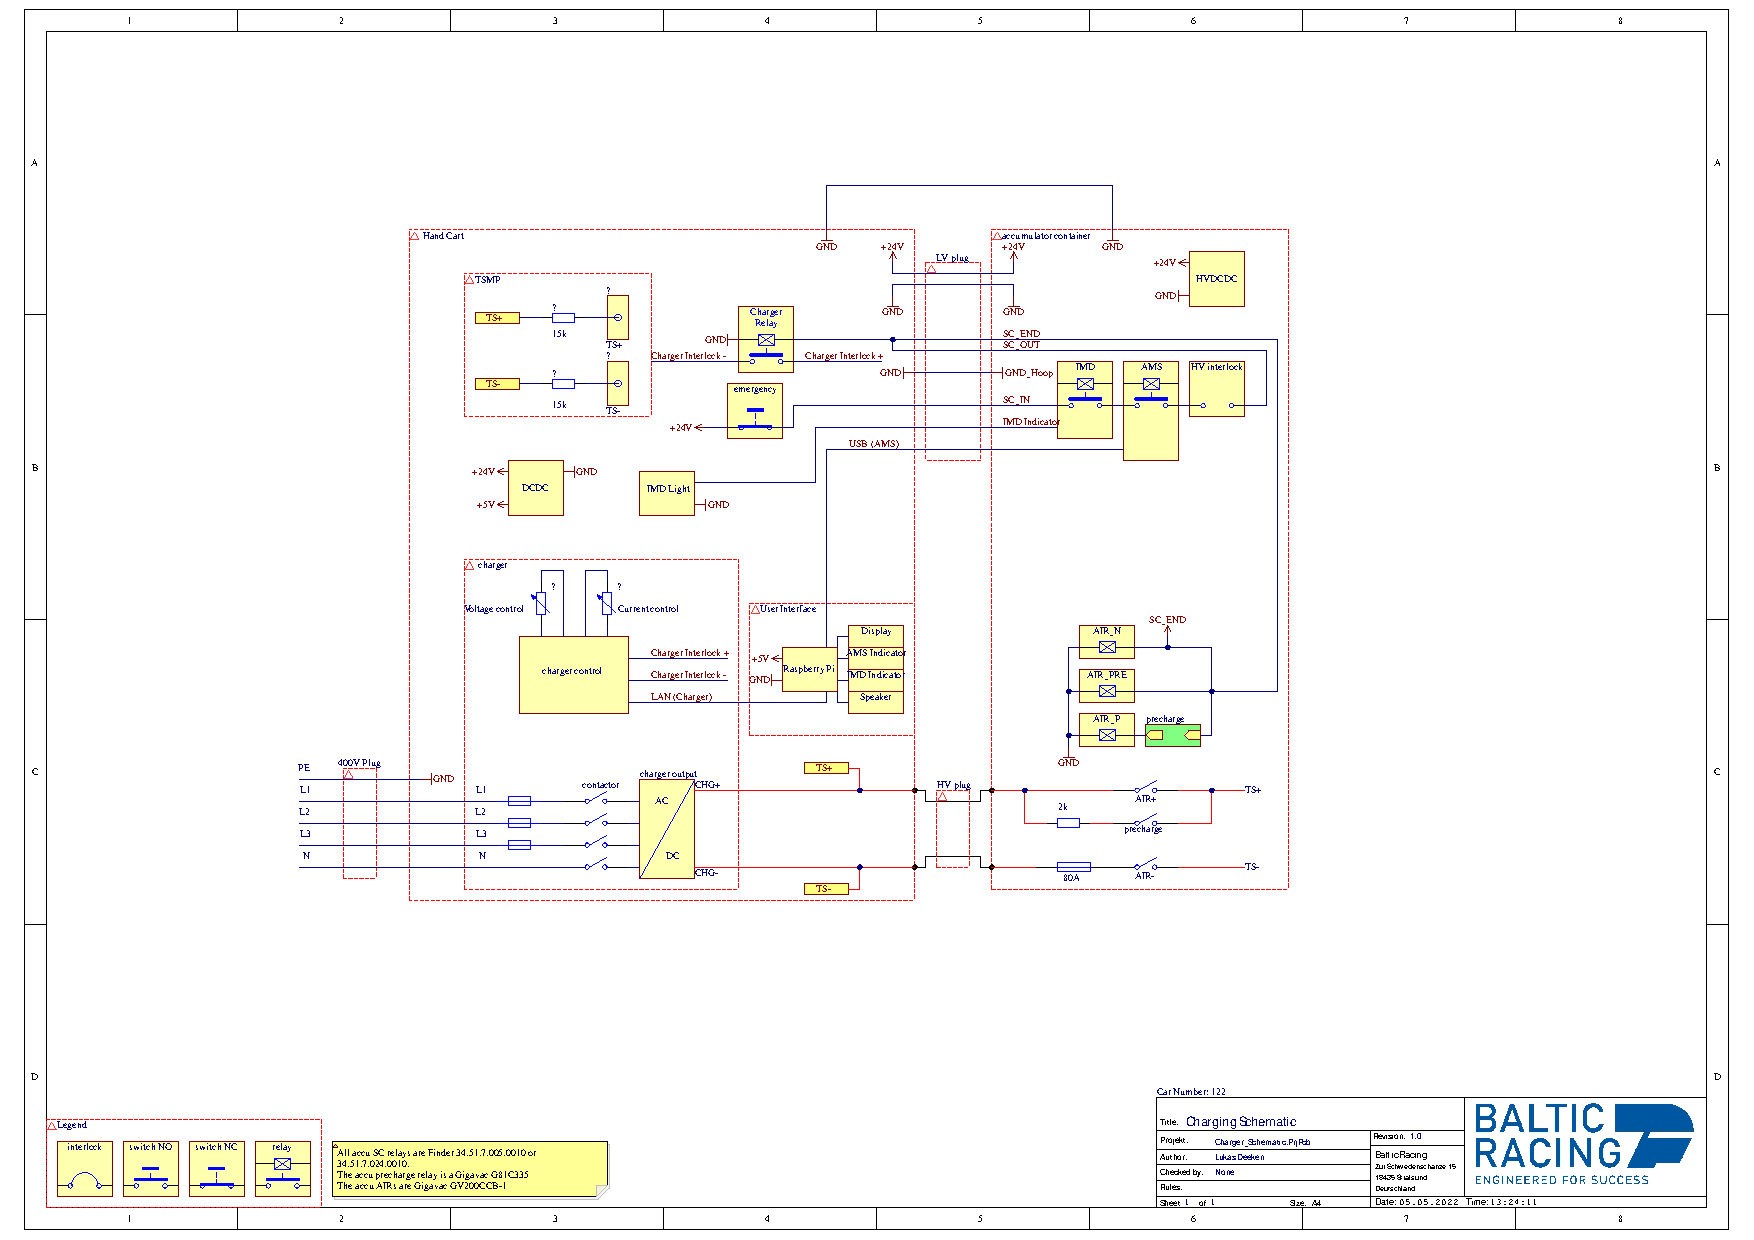
\includegraphics[width=1\linewidth]{C:/Users/lukas/Desktop/Charger_Schematic_V3}
	\caption{Schaltplan Handcart}
	\label{fig:chargerschematicv3}
\end{figure}

\FloatBarrier

	% Autor: Lukas Deeken
% Letzte Bearbeitung: 01.05.2022

\chapter{Mechanische Systeme}
An dieser Stelle geht mein Dank an Florian Irle, der obwohl er sich eigentlich etwas aus dem Projekt zurückhalten wollte, mit einem beispiellosen Tatendrang an der Entwicklung und Konstruktion des Antriebssysteme besonders des Getriebegehäuses und des Gussprozesses mitgearbeitet hat.

\section{Antriebslayout}
2WD ein motor (diff)
2Wd zwei motor (gewähltes konzept, Torque vektoring/hinterachslenkung)
4WD (Komplexität ungefederte massen etc.)

kurz was gibt es und warum machen wir das was wir machen

\section{Packaging}
Packaging leistungskennzahl. Volumenfüllungsgrad, schwerpunkt position, wartungsaufwand

\section{Systeme}

\subsection{Kühlung} (zusammen mit Julian Vogt und???)

\begin{figure}[H]
	\centering
	
\usetikzlibrary{arrows}
\begin{tikzpicture}
\tikzstyle{radiator} = [draw,outer sep=3,inner sep=3,line width=1, very thick, draw=black!55, top color=white,bottom color=blue!20]
\tikzstyle{Pumpe} = [draw,outer sep=3,inner sep=3,line width=1, very thick, draw=black!55, top color=white,bottom color=black!20]
\tikzstyle{Inverter} = [draw,outer sep=3,inner sep=3,line width=1, very thick, draw=black!55, top color=white,bottom color=orange!20]
\tikzstyle{Motor} = [draw,outer sep=3,inner sep=3,line width=1, very thick, draw=black!55, top color=white,bottom color=red!20]
\tikzstyle{Quickconnect} = [draw,outer sep=3,inner sep=3,line width=1, very thick, draw=black!55, top color=white,bottom color=yellow!20]

\node [radiator] (v7) at (-2,-2.5) {Radiator};
\node [radiator] (v8) at (1,-2.5) {Radiator};
\node [Pumpe] (v1) at (-0.5,-6.5) {Pumpe};
\node [Inverter] (v2) at (-2,-5.5) {Inverter};
\node [Inverter] (v3) at (1,-5.5) {Inverter};
\node [Motor] (v6) at (-2,-3.5) {Motor};
\node [Motor] (v5) at (1,-3.5) {Motor};
\node [Quickconnect] (v4) at (-0.5,-4.5) {QuickDC};
\node [Quickconnect] (v9) at (-0.5,-1.5) {QuickDC};

\tikzstyle{Leitungen} = [-triangle 60, color=blue]
\draw [Leitungen] (v1) edge (v2);
\draw [Leitungen] (v1) edge (v3);
\draw [Leitungen] (v2) edge (v4);
\draw [Leitungen] (v3) edge (v4);
\draw [Leitungen] (v4) edge (v5);
\draw [Leitungen] (v4) edge (v6);
\draw [Leitungen] (v6) edge (v7);
\draw [Leitungen] (v5) edge (v8);
\draw [Leitungen] (v7) edge (v9);
\draw [Leitungen] (v8) edge (v9);

\draw [Leitungen] (v9) -- (-0.5,-0.5) -- (-4,-0.5) -- (-4,-7.5) -- (-0.5,-7.5) -- (v1);
\end{tikzpicture}
	\caption{Kühlsystem Übersicht}
	\label{abb:Coolingssystem}
\end{figure}


\subsubsection{Radiator \& Lüfter} (zusammen mit Julian Vogt und???)
Radiator Berechnung
Die Berechnung des Radiators basiert auf der Annahme das hier eine Ähnlichkeitstheorie Anwendung finden kann. Hierbei wurden die bekannten realen (index r) Eingangsparameter aus Messungen am Vorjahresfahrzeug mit den Modellparametern (index m) für das kommende Fahrzeug in Beziehung gesetzt. Konkret die Temperaturdifferenz am eintritt und der Wärmestrom. Hierbei wurde kein klassischer Weg bekannt aus der Thermodynamik über NTU-Schaubilder etc. gewählt da die geometrischen Parameter des Radiators abgesehen von der frontalen Netzfläche nicht bekannt waren. Zur genaueren Betrachtung sollte dieses Vorgehen in Zukunft angewendet werden. Folgend die angewendete Formel.

\begin{equation}
		\label{eqn:KühlerÄhnlichkeitsformel}
		\dfrac {\glsc{symb:A_r}} {\glsc{symb:A_m}} = \dfrac {\glsc{symb:Qdot_r} * \glsc{symb:deltaT_ein r}} {\glsc{symb:Qdot_m} * \glsc{symb:deltaT_ein m}}
\end{equation}

Sie besagt, dass das Verhältnis der Kühlerflächen proportional zu dem Verhältnis von Wärmestrom und Eingangstemperaturdifferenz ist.\\

Hierbei ist \glsc{symb:A_r} vom Vorjahresfahrzeug bekannt, \glsc{symb:Qdot_r} ergibt sich mit folgender Formel aus den Vor und Rücklauftemperaturen vom Wärmetauscher sowie dem Wassermassenstrom welche beim TY19 gemessen wurden.

\begin{equation}
	\glsc{symb:Qdot_r} = \glsc{symb:Cv_wasser} * \glsc{symb:Vdot_wasser} * \glsc{symb:rho_wasser} * (\gls{symb:t_ein Wasser} - \glsc{symb:t_aus Wasser}) * Anzahl\textsubscript{Kühler}
\end{equation}

\glsc{symb:Qdot_m} wird mit Hilfe der Rundenzeitsimulation ermittelt. Hier werden sämtlich Verluste die in das Kühlsystem eingetragen im rahmen der Rundenzeit Berechnung über den FSG Fahrtzyklus gemittelt mit gerechnet.\\

\glsc{symb:deltaT_ein m} wird mit 30 K angenommen. Die max. Temperatur des Kühlwassers sollte 60°C nicht überschreiten währen im Hochsommer mit Umgebungstemperaturen von 30°C zu rechnen ist.\\

Mit der Formel \ref{eqn:KühlerÄhnlichkeitsformel} umgestellt nach \glsc{symb:A_m} kann nun die Kühlerfläche für das Elektrofahrzeug bestimmt werden.

\begin{equation}
	\glsc{symb:A_m} = \dfrac {\glsc{symb:A_r} * \glsc{symb:Qdot_m} * \glsc{symb:deltaT_ein m}} {\glsc{symb:Qdot_r} * \glsc{symb:deltaT_ein r}}
\end{equation}

Dies führt zu folgenden Ergebnissen.

\begin{table}[h]
	\centering
	\begin{tabular}{|c|c|c|}
		\hline
		\multicolumn{3}{|c|}{Eingangsparameter} \\
		\hline
		\glsc{symb:A_r} & 0,099 & \ensuremath{m^2} \\
		\hline
		\glsc{symb:t_ein Wasser} & 73,16 & °C \\
		\hline
		\glsc{symb:t_aus Wasser} & 70,37 & °C \\
		\hline
		\glsc{symb:rho_wasser} & 997 & \ensuremath{Kg/m^3} \\
		\hline
		\glsc{symb:Vdot_wasser} & 36,26 & \ensuremath{l/min} \\
		\hline
		\glsc{symb:Cv_wasser} & 4190 & \ensuremath{J/Kg K} \\
		\hline
		\glsc{symb:deltaT_ein r} & 43,16 & \ensuremath{K} \\
		\hline
		\glsc{symb:deltaT_ein m} & 30 & \ensuremath{K} \\
		\hline
		\glsc{symb:Qdot_m} & 5364 & \ensuremath{W} \\
		\hline
		\multicolumn{3}{|c|}{Ergebnisse} \\
		\hline
		\glsc{symb:Qdot_r} & 14089 & \ensuremath{W} \\
		\hline
		\glsc{symb:A_m} & 0,026 & \ensuremath{Kg/s} \\
		\hline
	\end{tabular}
\end{table}

Dies ergibt mit unserem Modell eine Reduktion auf 26,46 \% der vorherigen Kühlerfläche. Die Baugröße die am ende für den Kühler gewählt wurde entspricht ca. 50 \% der Kühlerfläche also das doppelte vom Rechenergebnis. Eine derart hohe Sicherheit ist darauf zurückzuführen das die Berechnung von Wärmeübertragern generell keine sehr exakte Wissenschaft ist und Der Bauraum eine derartige Überdimensionierung an der stelle zugelassen hat.\\
\\
Für die Auslegung des Lüfters wurde von der Aerodynamik Abteilung vorgegeben das man die Abluft des Systems nutzen möchte um das Strömungsprofil am Diffusor zu verwenden. Hierfür mussten Strömungsgeschwindigkeiten im Bereich der 80-90 km/h am Auslass erreicht werden. Für den Lüfter wurde auch in den letzten Jahren am Verbrenner ein Drohnennmotor mit Propeller und externer Ansteuerung verwendet da dies deutlich leichter ist als eine fertige Einheit. In diesem Zuge sollten Volumenstrom und Ausgangsgeschwindigkeiten für verschiedene Konzepte berechnet werden können. Aufgrund der Größe des Kühlers kamen nur 4 Zoll oder kleiner Propeller in Frage. Weiterhin ist die Fragestellung aufgekommen ob ein Propeller ausgelegt für Freiströmung sinnvoll vor einem Lamellen Kreuzstrom Wärmeübertrager einzusetzen ist. Hierfür wurde zum Vergleich ein Lüfter von der Firma EBM Papst beschafft um die Leistungsdaten schlussendlich vergleichen zu können.\\

Für drohnemotoren sind in der regel Daten für Schubkraft und Leistung verfügbar. Dies Lässt sich mit Hilfe des 2. Newtonschen Gesetztes dem Impulssatz umrechnen. Wir nehmen dabei an das unser Fahrzeug still steht. Dies führt zu folgender Gleichung

\begin{equation}
	\glsc{symb:F_Schub} = \glsc{symb:mdot_Luft} * \glsc{symb:v_Luft}
\end{equation}

Dies lässt sich mit folgenden Formeln Umstellen

\begin{equation}
	\glsc{symb:mdot_Luft} = \glsc{symb:Vdot_Luft} * \glsc{symb:rho_Luft}
\end{equation}
\begin{equation}
	\glsc{symb:Vdot_Luft} = \glsc{symb:A_Prop} * \glsc{symb:v_Luft}
\end{equation}

Und führt zu

\begin{equation}
	\glsc{symb:v_Luft} = \sqrt{\dfrac{\glsc{symb:F_Schub}} {\glsc{symb:A_Prop} * \glsc{symb:rho_Luft}}}
\end{equation}

Mit diesen Gleichungen können wir auch den Volumen- und Massenstrom bestimmen.\\

Mit folgender Formel lässt sich die Luftleistung bestimmen.

\begin{equation}
	\glsc{symb:P_Luft} = \dfrac{\glsc{symb:mdot_Luft}}{2} * \glsc{symb:v_Luft}^2
\end{equation}

Damit können wir schlussendlich die Effizienz des Design beurteilen

\begin{equation}
	\glsc{symb:eta_Lüfter} = \dfrac{\glsc{symb:P_Luft}}{\glsc{symb:P_elektrisch}}
\end{equation}

Entschieden wurde sich am ende für den T-Motor F2004-1700KV zusammen mit dem Gemfan 4023 Propeller. Daten dafür in folgender Tabelle.

\begin{table}[h]
\centering
\begin{tabular}{|c|c|c|}
	\hline
	\multicolumn{3}{|c|}{Eingangsparameter} \\
	\hline
	\glsc{symb:A_Prop} & 8107 & \ensuremath{mm^2} \\
	\hline
	\glsc{symb:F_Schub} & 650 & g \\
	\hline
	\glsc{symb:P_elektrisch} & 286 & W \\
	\hline
	\glsc{symb:rho_Luft} & 1,225 & \ensuremath{Kg/m^3} \\
	\hline
	\multicolumn{3}{|c|}{Ergebnisse} \\
	\hline
	\glsc{symb:v_Luft} & 25,339 & \ensuremath{m/s} \\
	\hline
	\glsc{symb:mdot_Luft} & 0,25 & \ensuremath{Kg/s} \\
	\hline
	\glsc{symb:Vdot_Luft} & 0,21 & \ensuremath{m^3/s} \\
	\hline
	\glsc{symb:P_Luft} & 80,79 & W \\
	\hline
	\glsc{symb:eta_Lüfter} & 28 & \% \\
	\hline
\end{tabular}
\end{table}

Im Rahmen der Systembetrachtung wurden am tatsächlichen Aufbau einige Messdaten genommen.
\begin{table}[h]
	\centering
	\begin{tabular}{|c|c|c|}
		\hline
		\multicolumn{3}{|c|}{T-Motor F2004} \\
		\hline
		\glsc{symb:v_Luft} & 75 & \ensuremath{km/h} \\
		\hline
		\glsc{symb:P_elektrisch} & 195 & \ensuremath{W} \\
		\hline
		\multicolumn{3}{|c|}{EBM Papst 3214jh4} \\
		\hline
		\glsc{symb:v_Luft} & 73 & \ensuremath{km/h} \\
		\hline
		\glsc{symb:P_elektrisch} & 50 & \ensuremath{W} \\
		\hline
	\end{tabular}
\end{table}

Mit Hilfe der Vorherigen Rechnung können wir nun den gleichen Rechenweg Rückwärts gehen um uns wieder alle übrigen Parameter zu berechnen. Die Lüftauströmfläche beträgt dabei \ensuremath{0,004173m^2}.

\begin{table}[h]
	\centering
	\begin{tabular}{|c|c|c|}
		\multicolumn{3}{|c|}{T-Motor F2004} \\
		\hline
		\glsc{symb:v_Luft} & 75 & \ensuremath{km/h} \\
		\hline		
		\glsc{symb:Vdot_Luft} & 0,087 & \ensuremath{m^3/s} \\
		\hline
		\glsc{symb:mdot_Luft} & 0,107 & \ensuremath{kg/s} \\
		\hline
		\glsc{symb:P_Luft} & 23,115 & \ensuremath{W} \\
		\hline
		\glsc{symb:eta_Lüfter} & 12 & \ensuremath{\%} \\
		\hline		
		\multicolumn{3}{|c|}{EBM Papst 3214jh4} \\
		\hline
		\glsc{symb:v_Luft} & 75 & \ensuremath{km/h} \\
		\hline
		\glsc{symb:Vdot_Luft} & 0,085 & \ensuremath{m^3/s} \\
		\hline
		\glsc{symb:mdot_Luft} & 0,104 & \ensuremath{kg/s} \\
		\hline
		\glsc{symb:P_Luft} & 21,315 & \ensuremath{W} \\
		\hline
		\glsc{symb:eta_Lüfter} & 43 & \ensuremath{\%} \\
		\hline		
	\end{tabular}
\end{table}

Laut EBM Papst liegen die zu erwartende effizienzen bei einem Axialgebläse im Bereich von 25\% - 65\%. Daran ist zu erkennen das unser aktueller Lüfter von EBM noch nicht die effizienteste Lösungen darstellt und unser Drohnenmotor eine sehr ineffiziente Lösung darstellt. Dennoch ein Aufbau mit Lüftern von EBM wiegt ca. 560g während der Aufbau mit Drohnennmotoren bei ca. 55g liegt. Allein diese gewichtsersparnis ist den einsatz dieses gebläses schon wert. Empfehlenswert wäre an der Stelle die Optimierung des Rotorblattes auf den vorliegenden Anwendungsfall.


\subsubsection{Wasserpumpe und Schläuche} (zusammen mit Julian Vogt und???)


Für die Auslegung des Wasserkreislaufes sind die Druckabfälle der einzelsysteme relevant hierfür eine systemüberischt

auf tikzedit grafik verlinken

Desweiteren sind für die betrachtung weitere Parameter relevant. Laut Motorhersteller liegt der optimale Wasservolumenstrom bei 6-8 \ensuremath{l/min}. Aus der Vorhergehenden Betrachtung geht hervor das die umzusetzende Wärmeleistung bei 5364W liegt. Der angepeilte Luftvolumenstrom durch einen Kühler beläuft sich auf 756 \ensuremath{m^3/h}.

Mit den folgenden beiden Diagrammen der Schwämmle GmbH\&Co. KG aus dem Leistungsdatenblatt für die ELW Serie lässt sich der Druckabfall über den Radiator bestimmen.  Wärmeleistung.

\begin{figure}[h]
	\centering
	\includegraphics[width=0.7\linewidth]{"bilder/ELW_Leistung über Volumenstrom"}
	\caption{}
	\label{fig:elwleistung-uber-volumenstrom}
\end{figure}

Unser angestrebter Radiator entspricht mit seiner Netzfläche am ehesten dem ELW3. Dies würde bei den bisher bekannten Betriebsdaten zu eine Kühlleistung von 90 W/K oder auch 2700W führen. Oder bei zwei Einheiten zu 5400W. Dies ist sehr nah an der angestrebten

\begin{figure}[h]
	\centering
	\includegraphics[width=0.7\linewidth]{"bilder/ELW-Druckabfall über Volumenstrom"}
	\caption{}
	\label{fig:elw-druckabfall-uber-volumenstrom}
\end{figure}

Die Grafik ist an dieser stelle etwas verwirrend da der ELW 2 und der ELW3 die Farben getauscht haben. Da es sich hierbei jedoch um die einzigen Daten handelt die aufgetrieben werden konnten wird an dieser stelle angenommen das Die grüne Linie für den ELW3 steht und die Lila Linie den ELW 2 darstellt. Dies ist die sichere anmahne da dies im zweifel zu einem zu hohen Druckabfall und damit einer Überdimensionierung der Anlage führt.\\
Anhand dieser Grafik kann also nun der Druckabfall zu einem entsprechenden Wasservolumenstrom abgelesen werden.

Für den Inverter gibt es im Datenblatt ein fertiges Diagramm.
\begin{figure}[h]
	\centering
	\includegraphics[width=0.7\linewidth]{"bilder/Druckabfall DTI500LC"}
	\caption{}
	\label{fig:cooling-characteristik}
\end{figure}

Für den Motor existieren leider nur Daten an einem einzigen Punkt. An den anderen verläufen ist jedoch in der regel ein quadratischer verlauf zu erkennen weswegen hier quadratisch regressiert wurde. Wir beginnen mit der allgemeine Formel

\begin{equation}
	Y = A x^2 + B x + C
\end{equation}

Die Linie soll durch den Nullpunkt verlaufen damit wird C = 0 und wir nehmen an das es keinen linearen Anteil gibt, damit wird B = 0. Unsere Gleichung vereinfacht sich zu.

\begin{equation}
	Y = A x^2
\end{equation}

eingesetzt ergibt sich

\begin{equation}
	0,6 bar = A * (7 l/min)^2  
\end{equation}
\begin{equation}
	A = \dfrac{0,6 bar}{(7 l/min)^2 }
	  = 0,01224 \dfrac{bar}{(l/min)^2}
\end{equation}

Für die Leitungen würde eine extensive Berechnung durchgeführt auf die an dieser stelle leider aus zeit gründen nicht näher eingegangen werden kann. die Schlussfolgerung ist jedoch das die Verluste vernachlässigbar klein sind. \\

Die Daten für die Pumpen entstammen direkt den Datenblättern.\\

Alle Ergebnisse sind nun in der Systemkennlinie abgebildet

\begin{figure}[h]
	\centering
	\includegraphics[width=0.7\linewidth]{bilder/Kühlsystemkennlinie}
	\caption{}
	\label{fig:kuhlsystemkennlinie}
\end{figure}

Der Punkt an dem sich die Linien der jeweiligen Pumpe mit der Linie des Gesamtsystem schneidet ist der Betriebspunkt des Systems. Dieser Druckabfall und dieser Volumenstrom sollten sich im betrieb einstellen. Bei der Grafik muss beachtet werden das dies von der Pumpe beachtet aus betrachtet wird und daher der Volumenstrom doppelt so groß ist wie am kühler aufgrund der zwei separaten Kühleinheiten.


\subsection{Antrieb} (Michel und Linus)
zahnrad auslegung
Zahnrad fertigung
Kettentrieb alternative
Wellen auslegung
FEM detour

\subsubsection{Outbound vs Inbound}
Radnabenmotor vs interner motor 
	ungeferte massen
	packaging im rad problem(Planetengetriebe) fertigungsaufwand innenzahnkranz, generell zahnräder
	keine Antriebswellen
	besseres packaging im auto

\subsubsection{Gussgehäuse vs Fräsgehäuse vs Schweißgehäuse} (Flo Irle)
Vor und nachteile

eingehen aufs gussgehäuse

SES anforderungen
Flexural rigidity
E modul vs yield strenght welche verbnesserungen bringen wo was
Gussimulation
FEM Bilder
CAD Bilder
Formkasten
Heizofen
tiegel
trageschere
gussmaterial auswahl
kellen etc. für zusätze
wärmebehandlung
materialtests
zusatzstoffe guss
stuff von Floh?


\subsubsection{Antriebswellen und Tripoden} Störle und schrang
excel tabellen und stuff von Störle und schrang

FEM sim bilder von Schrang
FEM konvergenz
netzunabhängigkeit
Kräfte richtig antragen
Feste flächen richtig wählen
kräfte richtig berechnen
Kontaktflächen bestimmen
Feinheitsgrade des netz
Inventor Casual fixe abschätzung oder einfache probleme vs Ansys Profi tool für komplexe verlässliche analyse

	
	
	
	\appendix
	\part*{Anhang}
	\pagenumbering{Roman}
	\chapter{Erster Anhang}
	Beispieltext
	
	%% ++++++++++++++++++++++++++++++++++++++++++++++++++++++++++++
%% Anhang: Beispielkapitel "Messwerte"
%% ++++++++++++++++++++++++++++++++++++++++++++++++++++++++++++
%
%  Gerüst:
%  * Version 0.10
%  * Dipl.-Ing. Florian Evers, florian.evers@tu-ilmenau.de
%  * Fachgebiet Kommunikationsnetze, TU Ilmenau
%
%  Für Hauptseminare, Studienarbeiten, Diplomarbeiten
%
%  Autor           : Max Mustermann
%  Letzte Änderung : 31.12.2004
%

\section{Excel Dokumente}
Doppelklick auf das Symbol zum Öffnen.\\
\\
Kühlsystem Gesamtberechnung.xlsx
\attachfile[mimetype=application/vnd.ms-excel, icon=Paperclip]{calc/Kühlsystem_Gesamtberechnung_Lukas_Final.xlsx}

DC Converter Berechnung.xlsx
\attachfile[mimetype=application/vnd.ms-excel, icon=Paperclip]{calc/DC_Converter_Calc.xlsx}

Temperaturmodell Akku.xlsx
\attachfile[mimetype=application/vnd.ms-excel, icon=Paperclip]{calc/Temperaturmodell_Akku.xlsx}

Zellauswahl.xlsx
\attachfile[mimetype=application/vnd.ms-excel, icon=Paperclip]{calc/Zellauswahl_Master.xlsx}

	
%% ++++++++++++++++++++++++++++++++++++++++++++++++++++++++++++
%% Anhang: Beispielkapitel "Protokoll"
%% ++++++++++++++++++++++++++++++++++++++++++++++++++++++++++++
%
%  Gerüst:
%  * Version 0.10
%  * Dipl.-Ing. Florian Evers, florian.evers@tu-ilmenau.de
%  * Fachgebiet Kommunikationsnetze, TU Ilmenau
%
%  Für Hauptseminare, Studienarbeiten, Diplomarbeiten
%
%  Autor           : Max Mustermann
%  Letzte Änderung : 31.12.2004
%

\section{Schaltpläne}
\subsection{\ac{AMS}-Slave}
\includepdf[pages=-]{Schaltplaene/AMS_Slave_Passiv_V2.pdf}
\subsection{\ac{BSPD} System}
\includepdf[pages=-]{Schaltplaene/BSPD_Schematic_w_System_2.pdf}
\subsection{Chager}
\includepdf[pages=-]{Schaltplaene/Charger_Schematic_V3.pdf}
\subsection{\ac{HV}-DCDC}
\includepdf[pages=-]{Schaltplaene/HV_DCDC.pdf}
\subsection{HV-Distribution}
\includepdf[pages=-]{Schaltplaene/hv-distribution-board.pdf}
\subsection{\ac{SDC}}
\includepdf[pages=-]{Schaltplaene/Shutdowncircuit.pdf}
\subsection{\ac{TS}-System-Schematic}
\includepdf[pages=-]{Schaltplaene/Tractive_System_Schematic_V4.pdf}
\subsection{\ac{AMS}-Master}
\includepdf[pages=-]{Schaltplaene/tsac-distribution.pdf}
\subsection{\ac{TSAL}}
\includepdf[pages=-]{Schaltplaene/tsal.pdf}

	
	\chapter{Zweiter Anhang}
	Beispieltext
	
	%% ++++++++++++++++++++++++++++++++++++++++++++++++++++++++++++
%% Anhang: Beispielkapitel "Programm A"
%% ++++++++++++++++++++++++++++++++++++++++++++++++++++++++++++
%
%  Gerüst:
%  * Version 0.11
%  * Dipl.-Ing. Karsten Renhak, karsten.renhak@tu-ilmenau.de
%  * Fachgebiet Kommunikationsnetze, TU Ilmenau
%
%  Für Hauptseminare, Studienarbeiten, Diplomarbeiten
%
%  Autor           : Max Mustermann
%  Letzte Änderung : 31.12.2011
%

\section{Software A}
Beispieltext

	%% ++++++++++++++++++++++++++++++++++++++++++++++++++++++++++++
%% Anhang: Beispielkapitel "Programm B"
%% ++++++++++++++++++++++++++++++++++++++++++++++++++++++++++++
%
%  Gerüst:
%  * Version 0.11
%  * Dipl.-Ing. Karsten Renhak, karsten.renhak@tu-ilmenau.de
%  * Fachgebiet Kommunikationsnetze, TU Ilmenau
%
%  Für Hauptseminare, Studienarbeiten, Diplomarbeiten
%
%  Autor           : Max Mustermann
%  Letzte Änderung : 31.12.2011
%

\section{Software B}
Beispieltext

		
	% Literaturverzeichnis einbinden
	%% ++++++++++++++++++++++++++++++++++++++++++++++++++++++++++++
%% Anhang: Literaturverzeichnis
%% ++++++++++++++++++++++++++++++++++++++++++++++++++++++++++++
%
%  Gerüst:
%  * Version 0.11
%  * Dipl.-Ing. Karsten Renhak, karsten.renhak@tu-ilmenau.de
%  * Fachgebiet Kommunikationsnetze, TU Ilmenau
%
%  Für Hauptseminare, Studienarbeiten, Diplomarbeiten
%
%  Autor           : Max Mustermann
%  Letzte Änderung : 31.12.2011
%

% Mit dem Befehl \nocite werden auch nicht im Text zitierte
% aus der Literaturdatenbank mit in das Literaturverzeichnis aufgenommen.
% Ein "\nocite{*}" übernimmt ungeprüft die komplette Datenbank.
%\nocite{*}

\cleardoublepage
\ihead[]{Literaturverzeichnis}
\bibliographystyle{alphadin}
\bibliography{literatur} % "literatur.bib" ist hier die einzige Literaturdatenbank.
% Alternativ: Mehrere Datenbanken verwenden, falls eine
% oder mehrere umfangreiche Sammlungen exisitieren:
%\bibliography{literatur_buecher,literatur_weblinks}

	
\end{document}

